\begin{sidewaysfigure}
        \centering
        \begin{subfigure}[b]{0.2\textwidth}
                \centering
                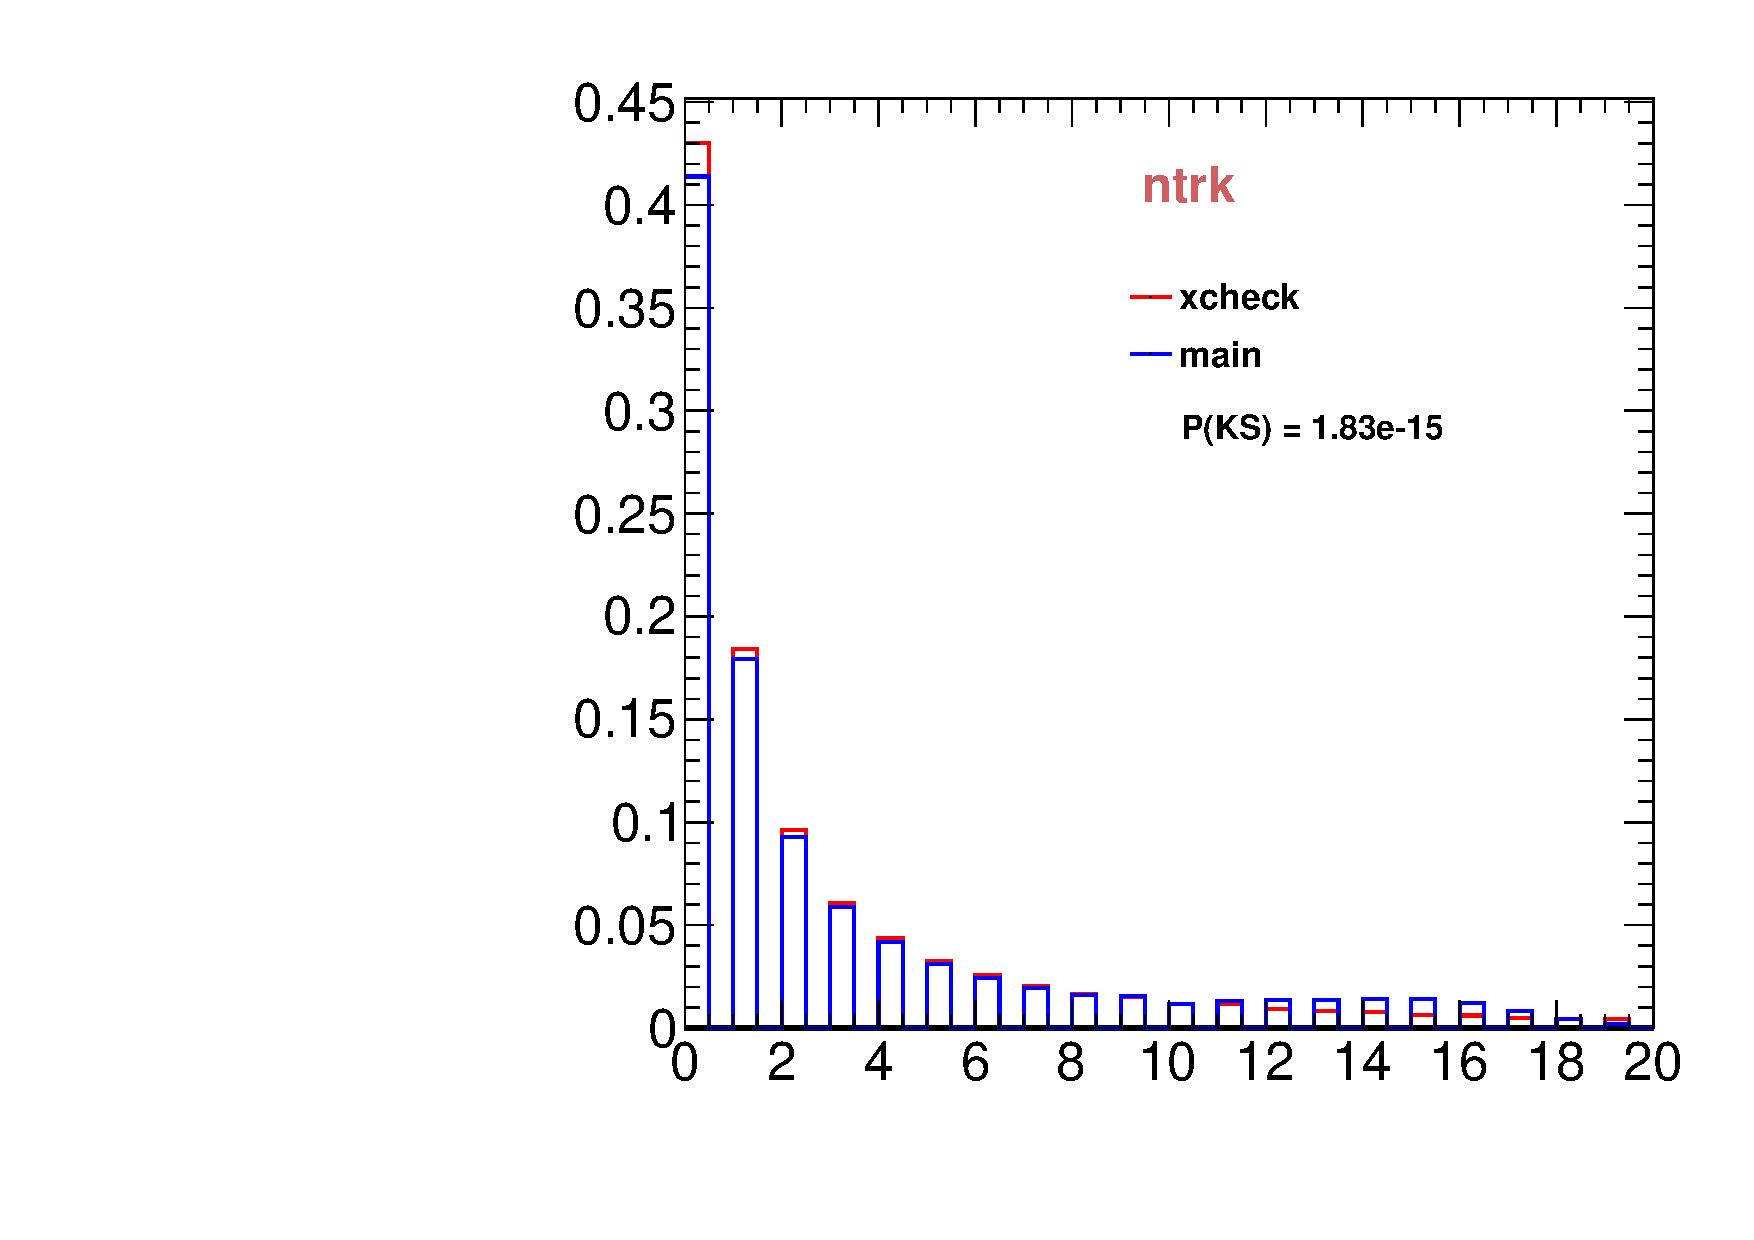
\includegraphics[width=\textwidth]{Figures/VariablesComparison/MC_barrel_figs/closetrk}
                \label{fig:MC_barrel_closetrk}
        \end{subfigure}
        \begin{subfigure}[b]{0.2\textwidth}
                \centering
                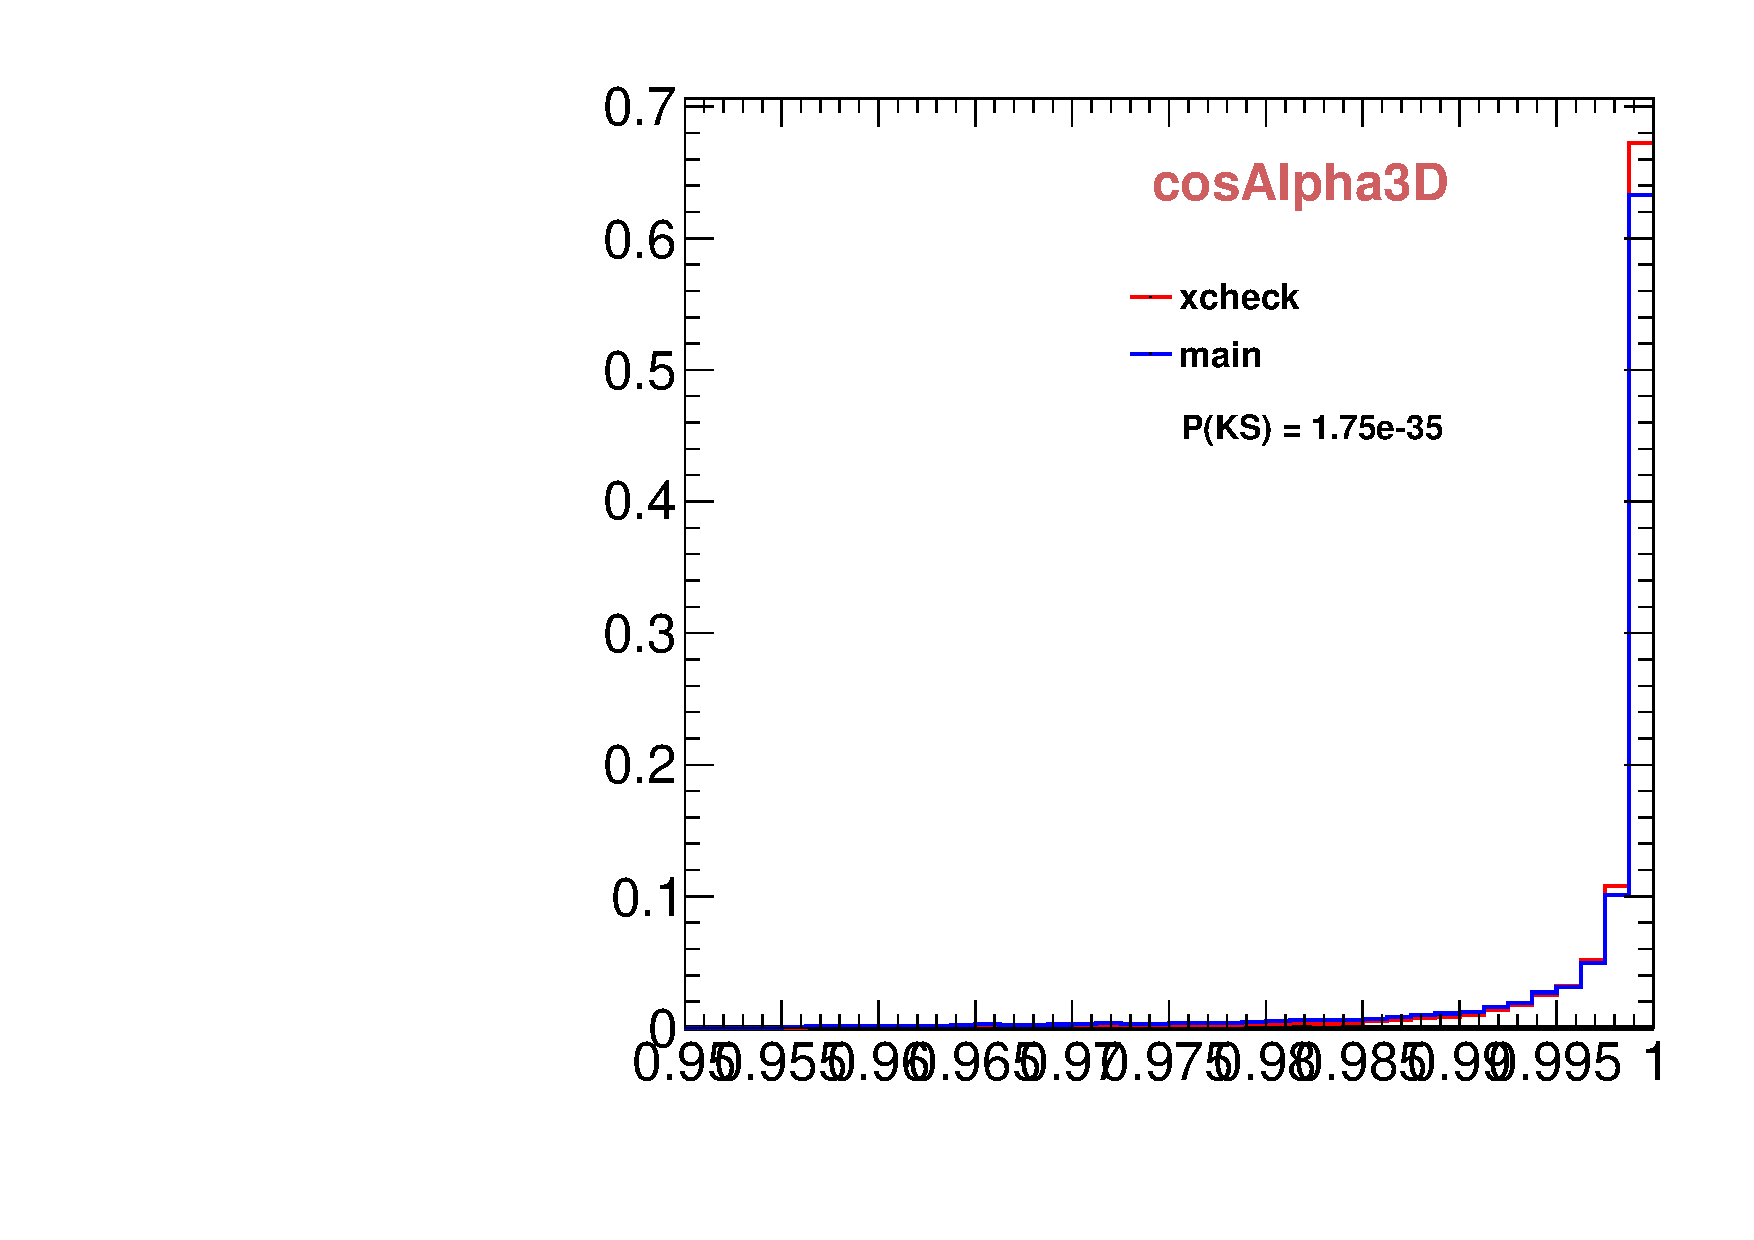
\includegraphics[width=\textwidth]{Figures/VariablesComparison/MC_barrel_figs/cosa}
                \label{fig:MC_barrel_cosa}
        \end{subfigure}
        \begin{subfigure}[b]{0.2\textwidth}
                \centering
                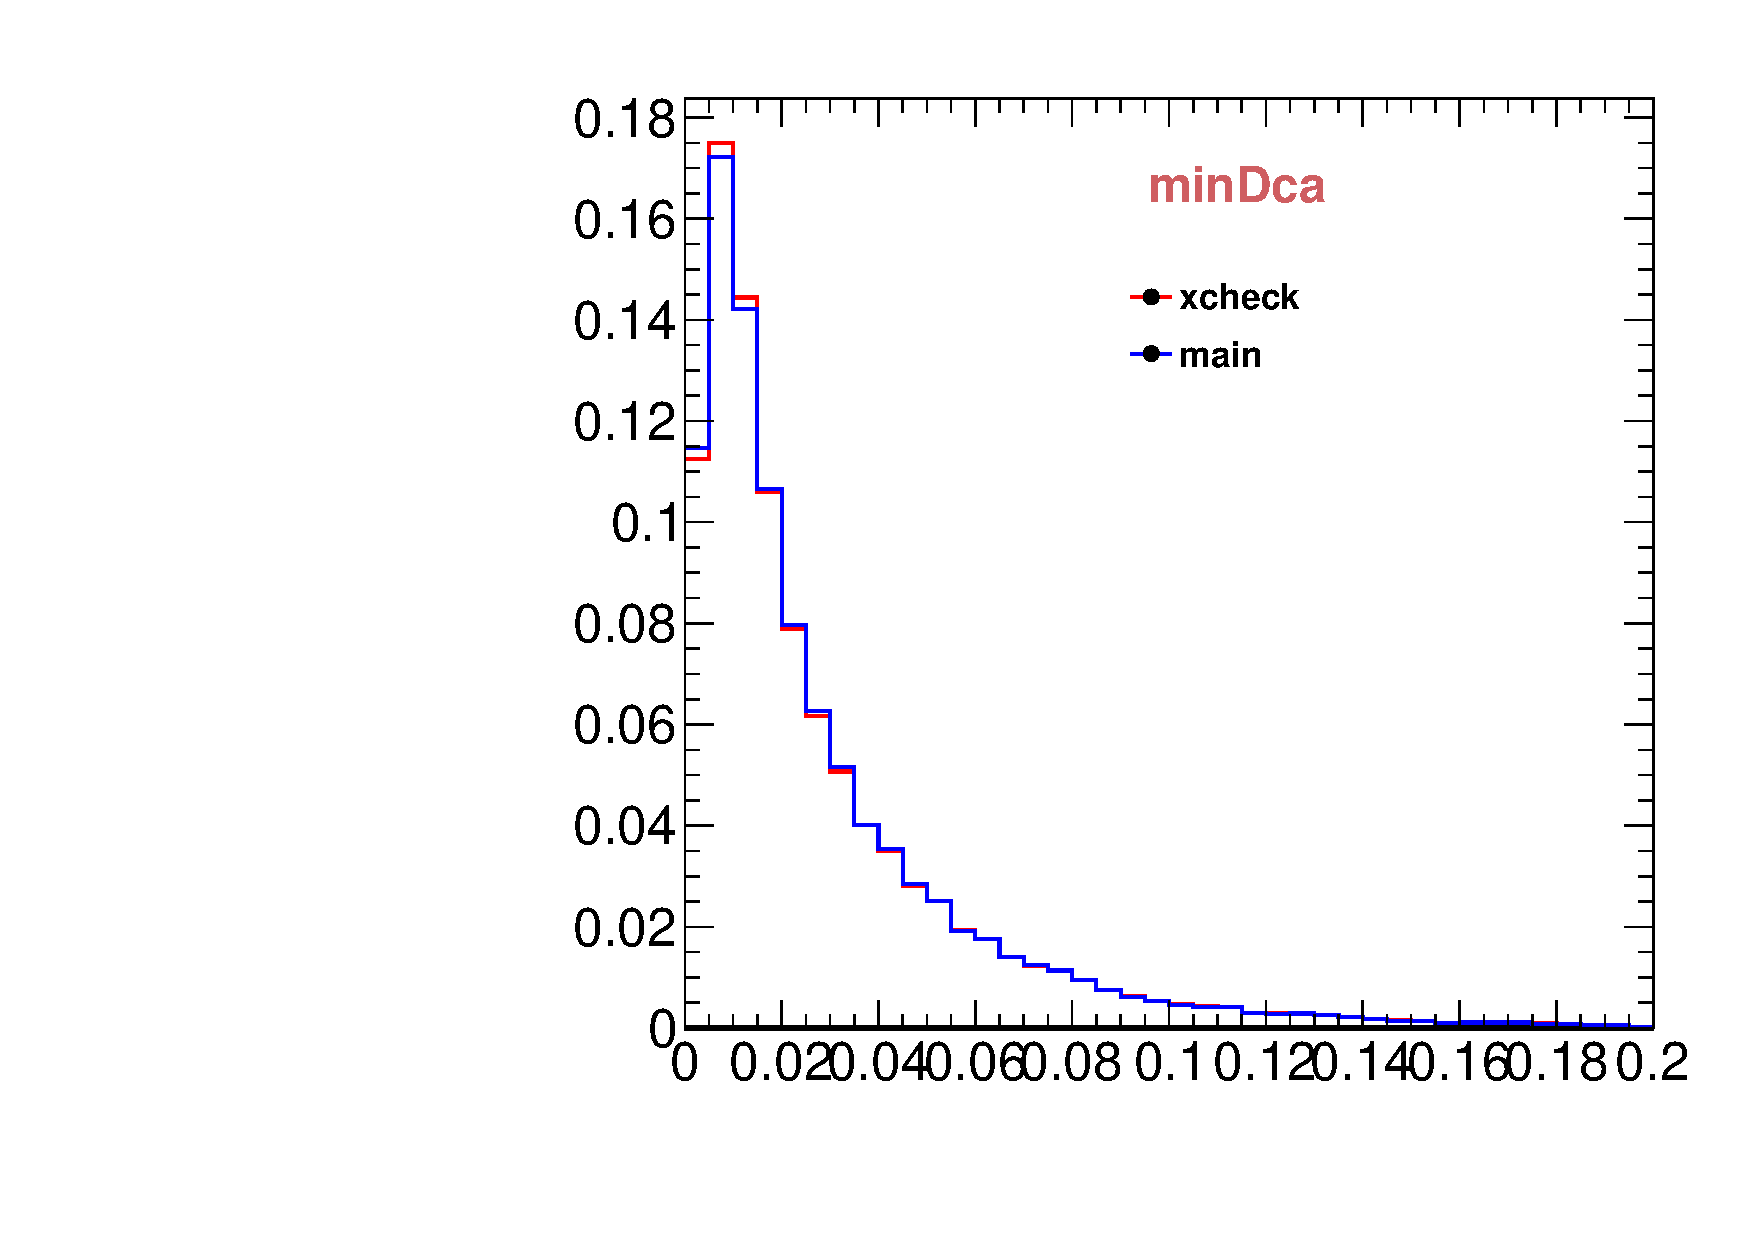
\includegraphics[width=\textwidth]{Figures/VariablesComparison/MC_barrel_figs/docatrk}
                \label{fig:MC_barrel_docatrk}
        \end{subfigure}
        \begin{subfigure}[b]{0.2\textwidth}
                \centering
                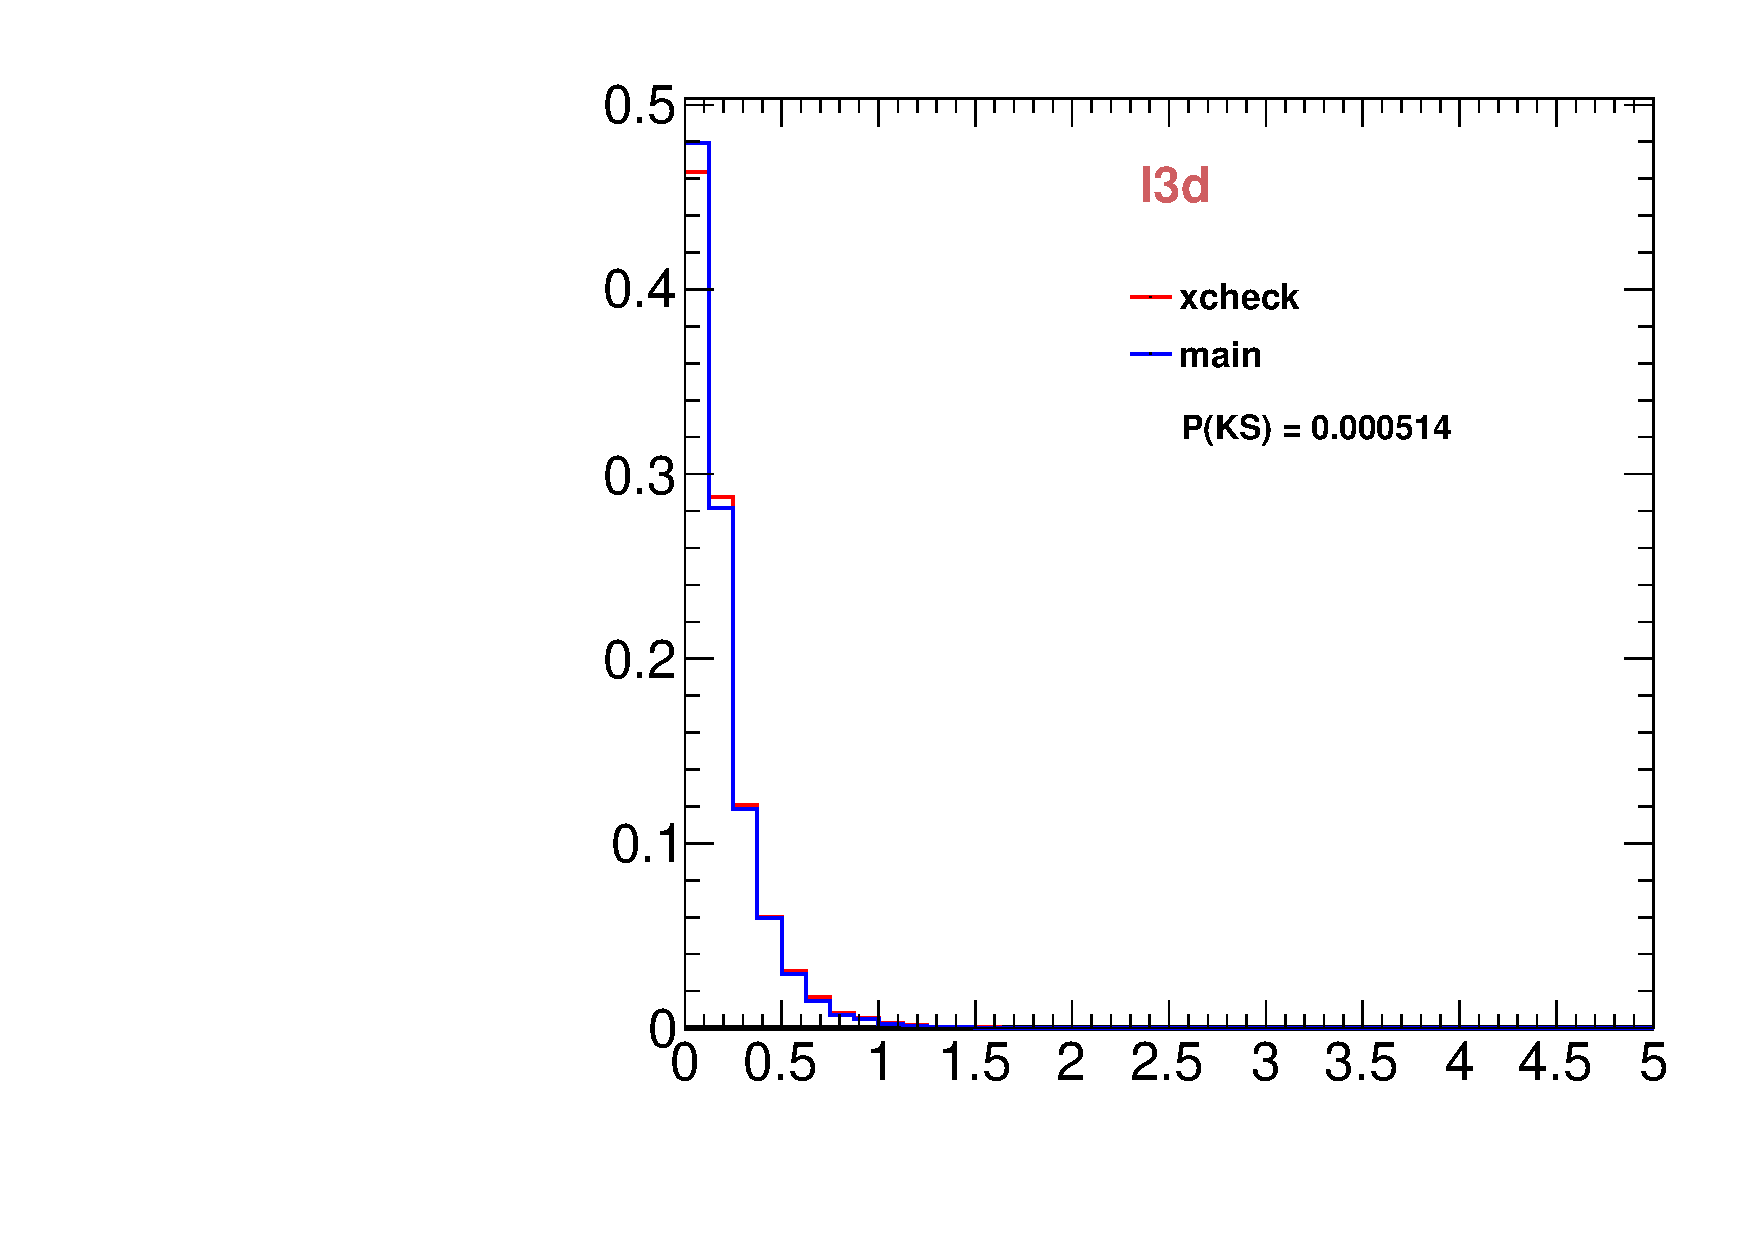
\includegraphics[width=\textwidth]{Figures/VariablesComparison/MC_barrel_figs/fl3d}
                \label{fig:MC_barrel_fl3d}
        \end{subfigure}
        \begin{subfigure}[b]{0.2\textwidth}
                \centering
                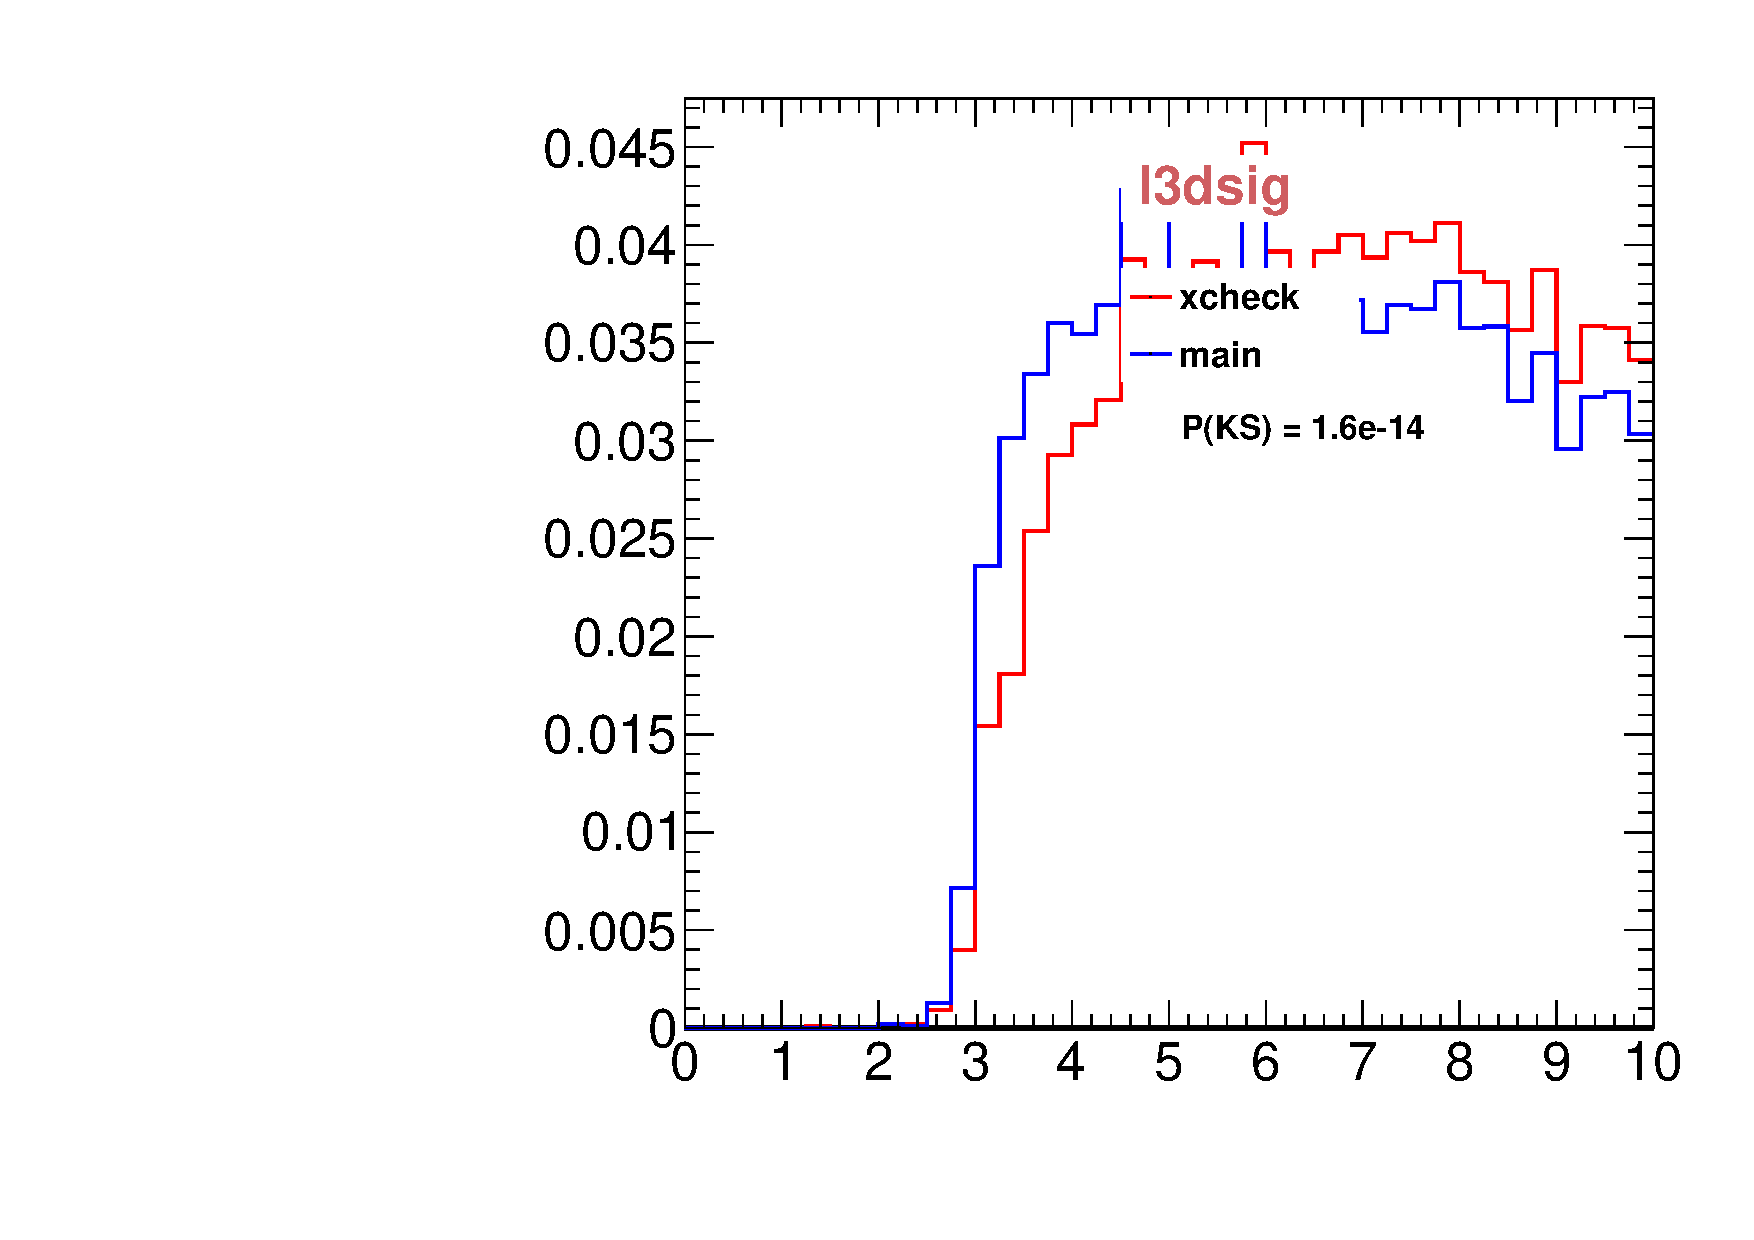
\includegraphics[width=\textwidth]{Figures/VariablesComparison/MC_barrel_figs/fls3d}
                \label{fig:MC_barrel_fls3d}
        \end{subfigure}
        \begin{subfigure}[b]{0.2\textwidth}
                \centering
                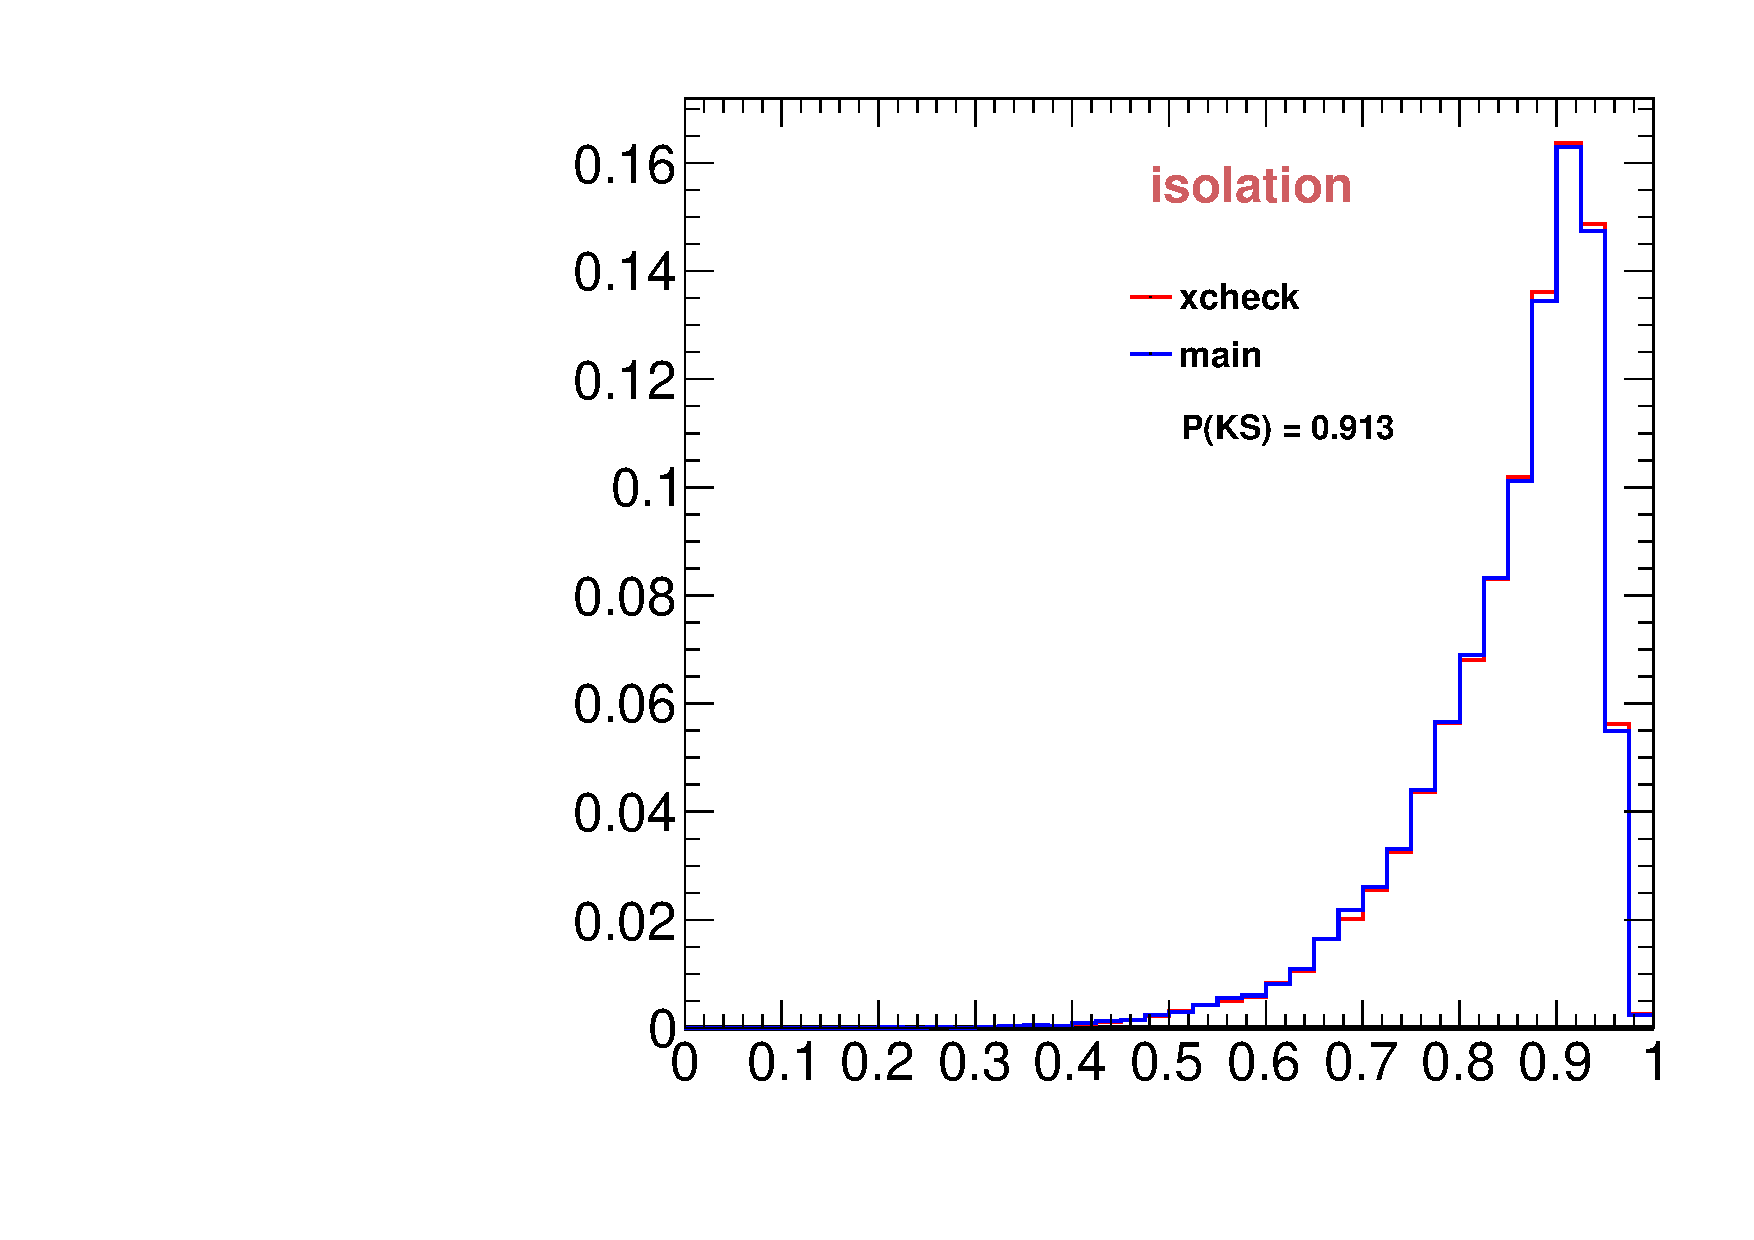
\includegraphics[width=\textwidth]{Figures/VariablesComparison/MC_barrel_figs/iso}
                \label{fig:MC_barrel_iso}
        \end{subfigure}
        \begin{subfigure}[b]{0.2\textwidth}
                \centering
                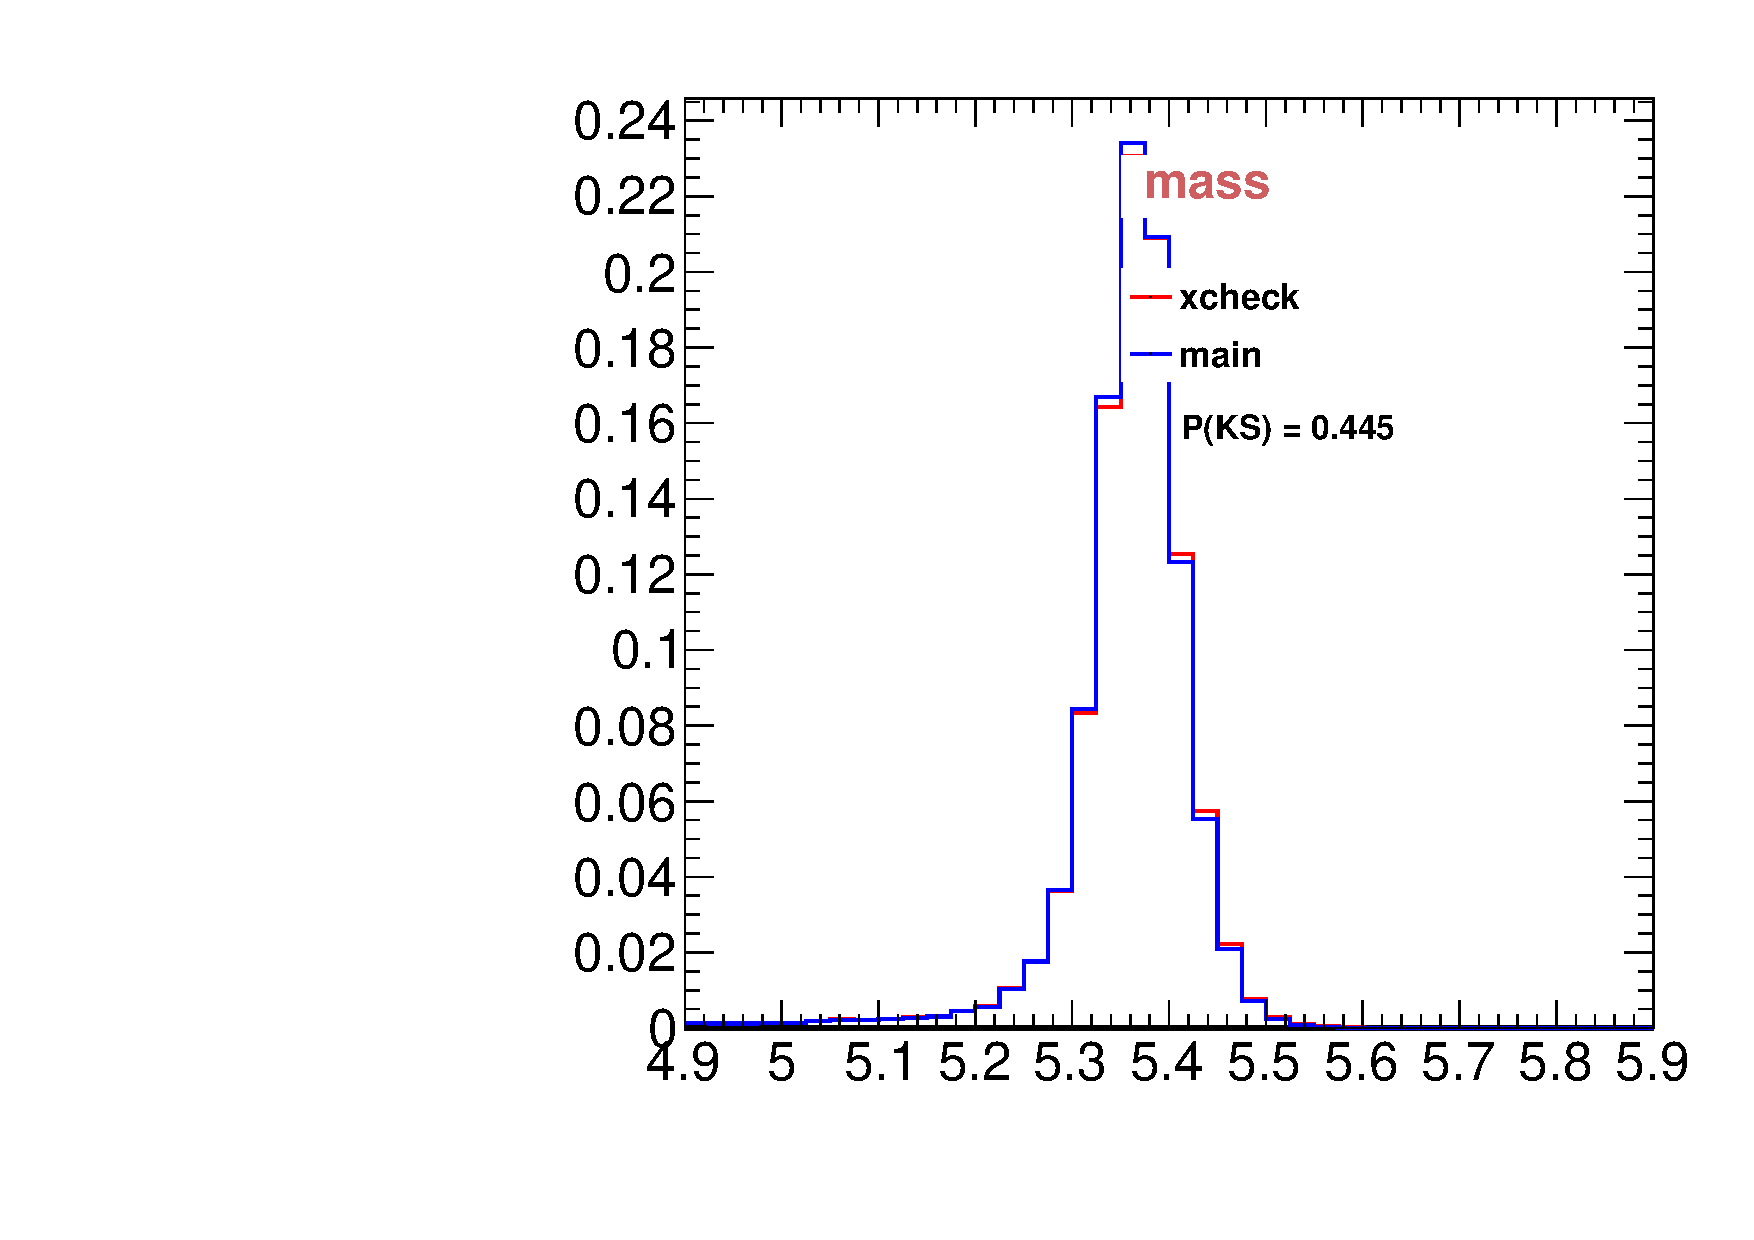
\includegraphics[width=\textwidth]{Figures/VariablesComparison/MC_barrel_figs/m}
                \label{fig:MC_barrel_m}
        \end{subfigure}
        \begin{subfigure}[b]{0.2\textwidth}
                \centering
                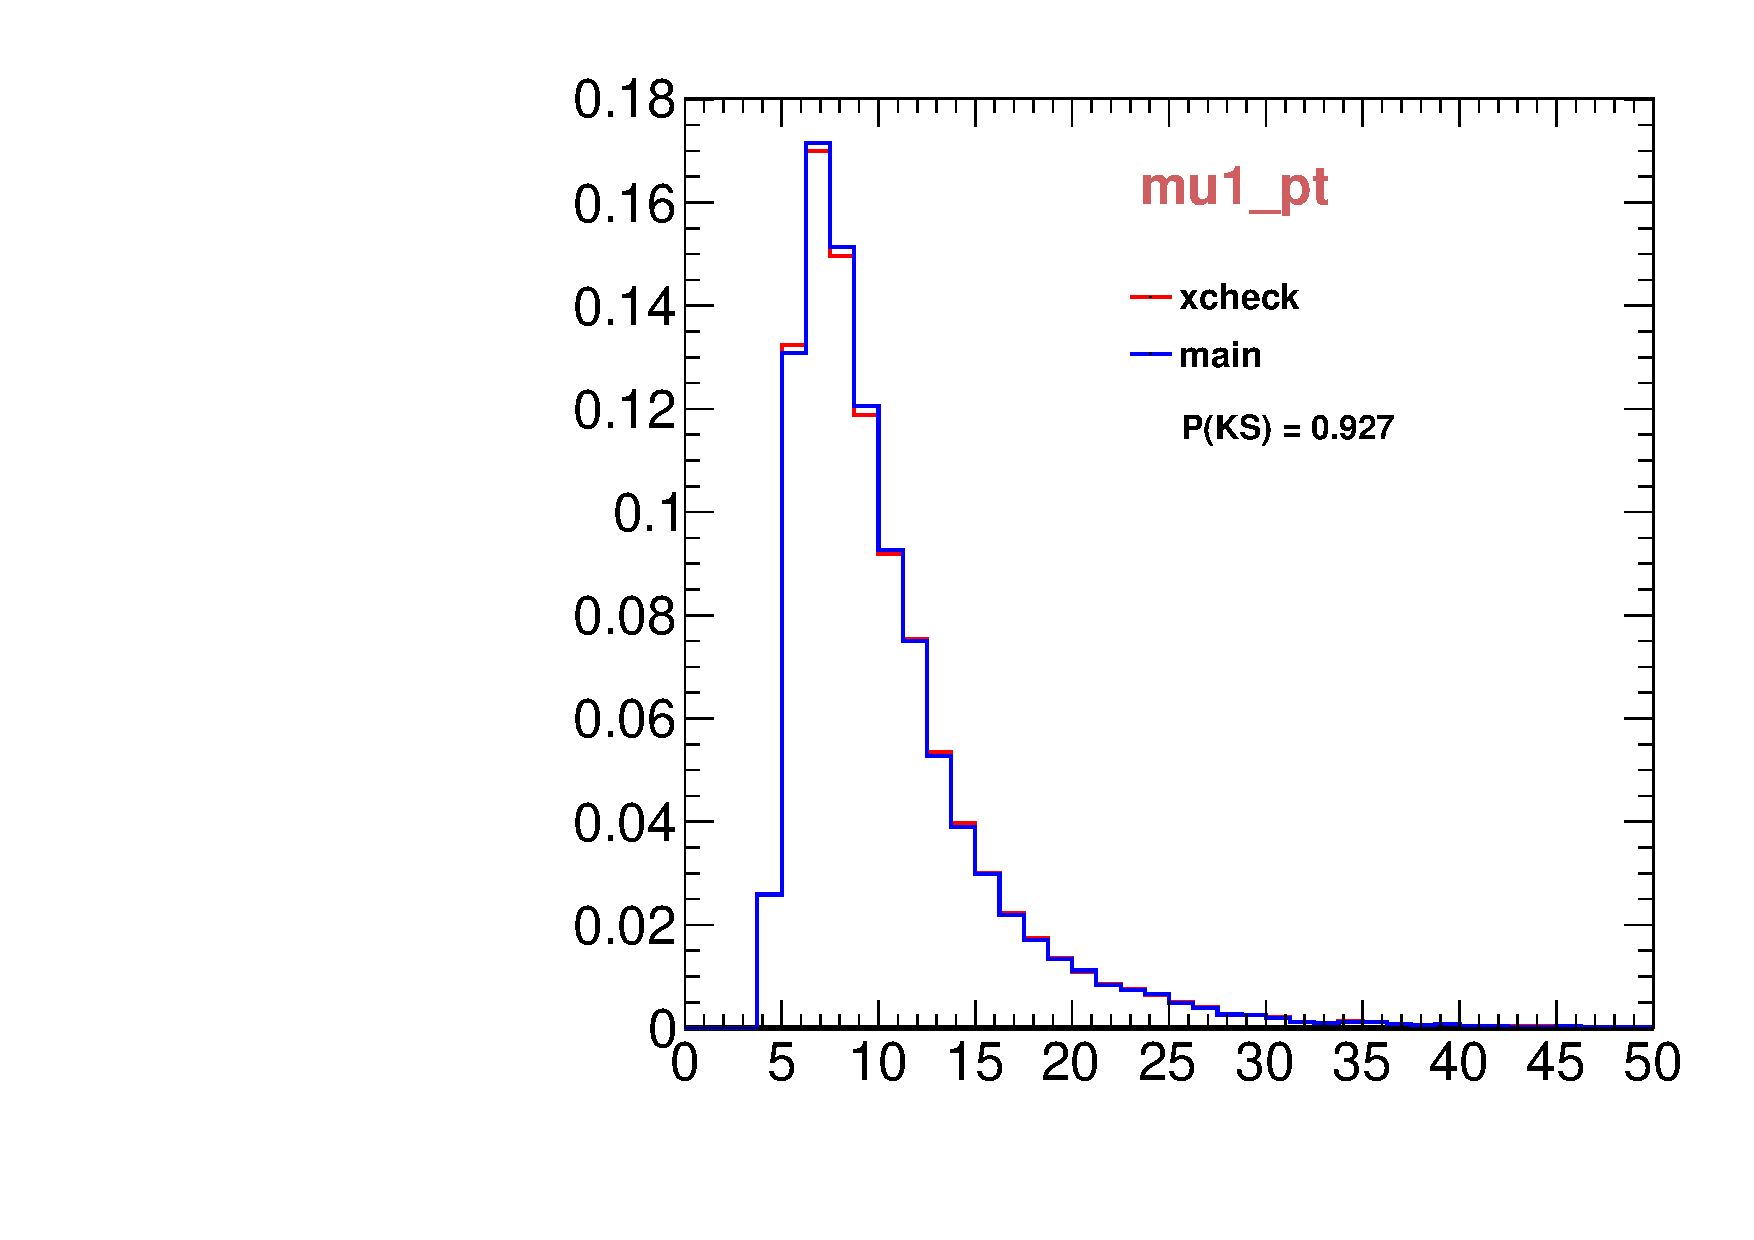
\includegraphics[width=\textwidth]{Figures/VariablesComparison/MC_barrel_figs/m1pt}
                \label{fig:MC_barrel_m1pt}
        \end{subfigure}
        \begin{subfigure}[b]{0.2\textwidth}
                \centering
                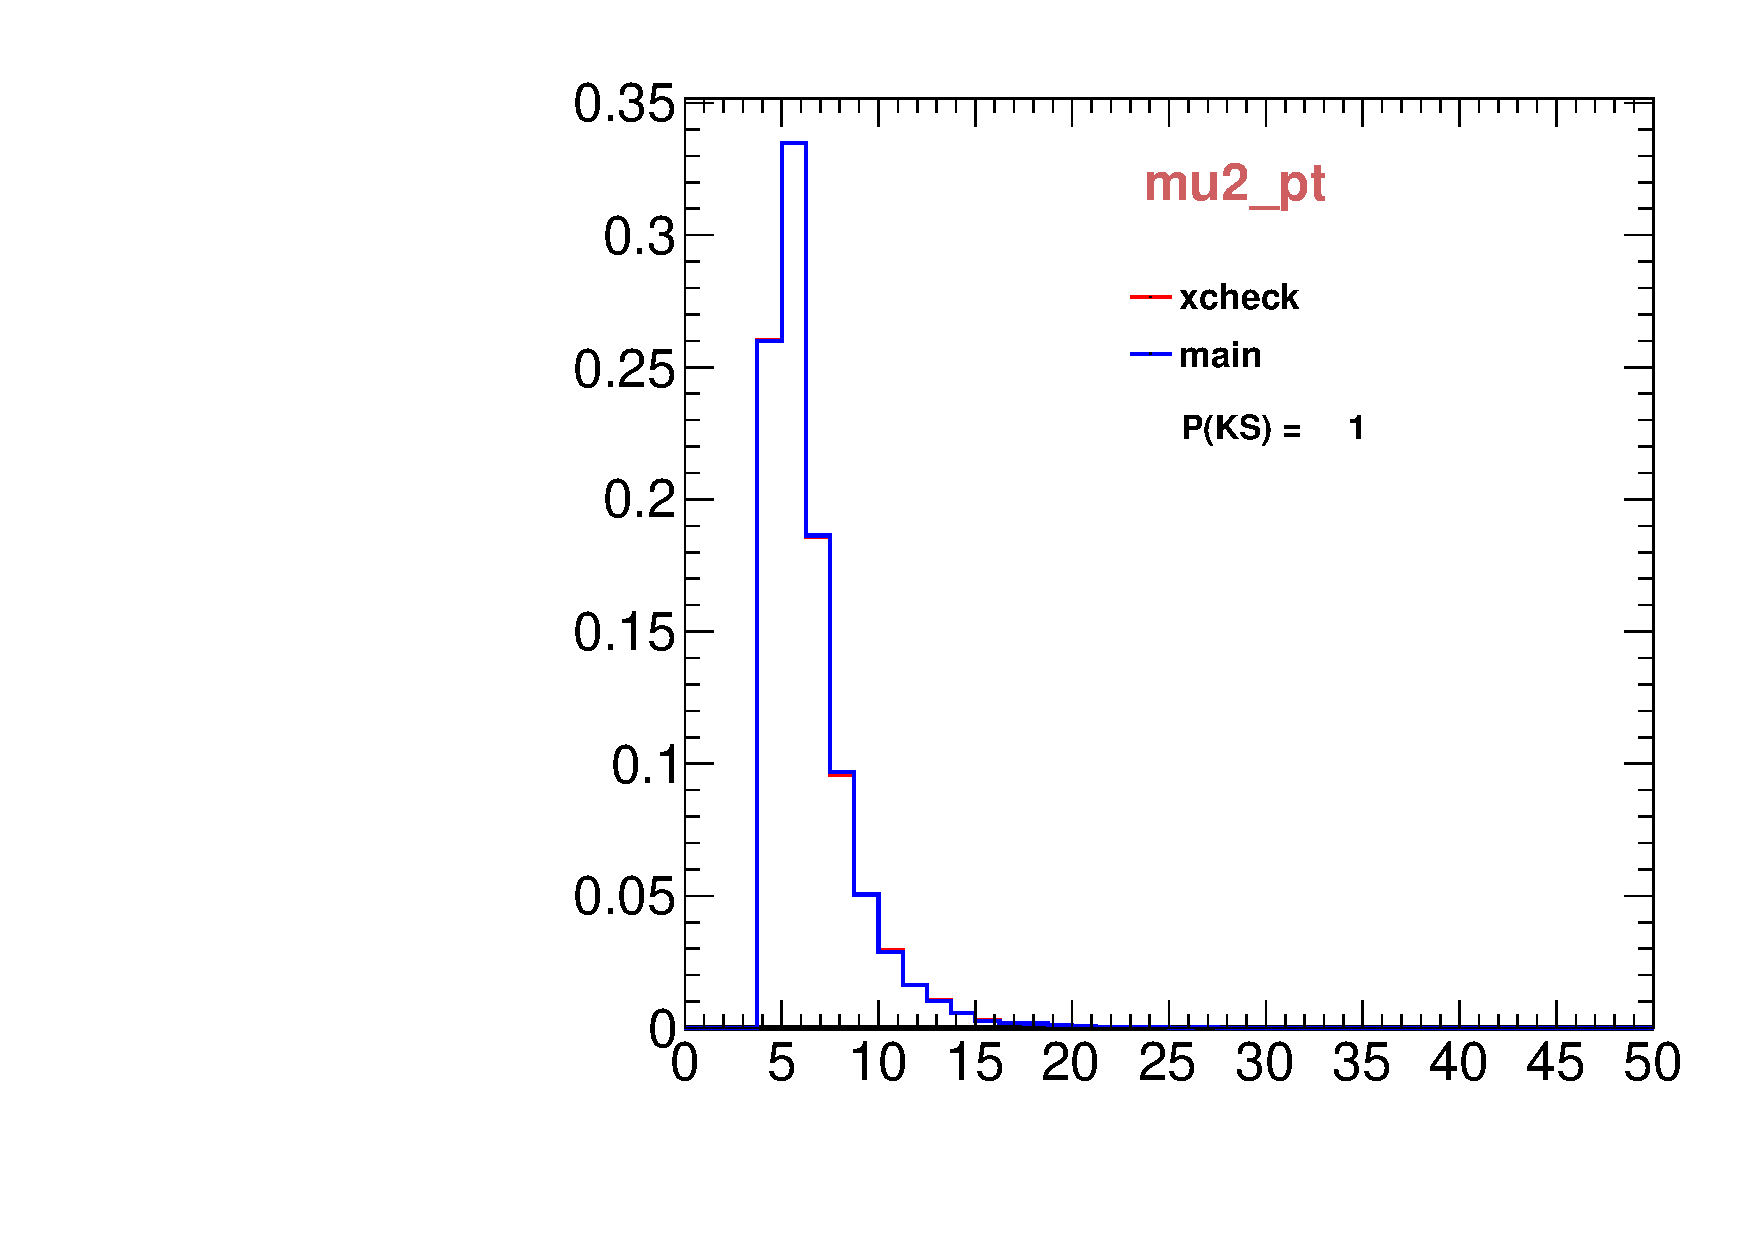
\includegraphics[width=\textwidth]{Figures/VariablesComparison/MC_barrel_figs/m2pt}
                \label{fig:MC_barrel_m2pt}
        \end{subfigure}
        \begin{subfigure}[b]{0.2\textwidth}
                \centering
                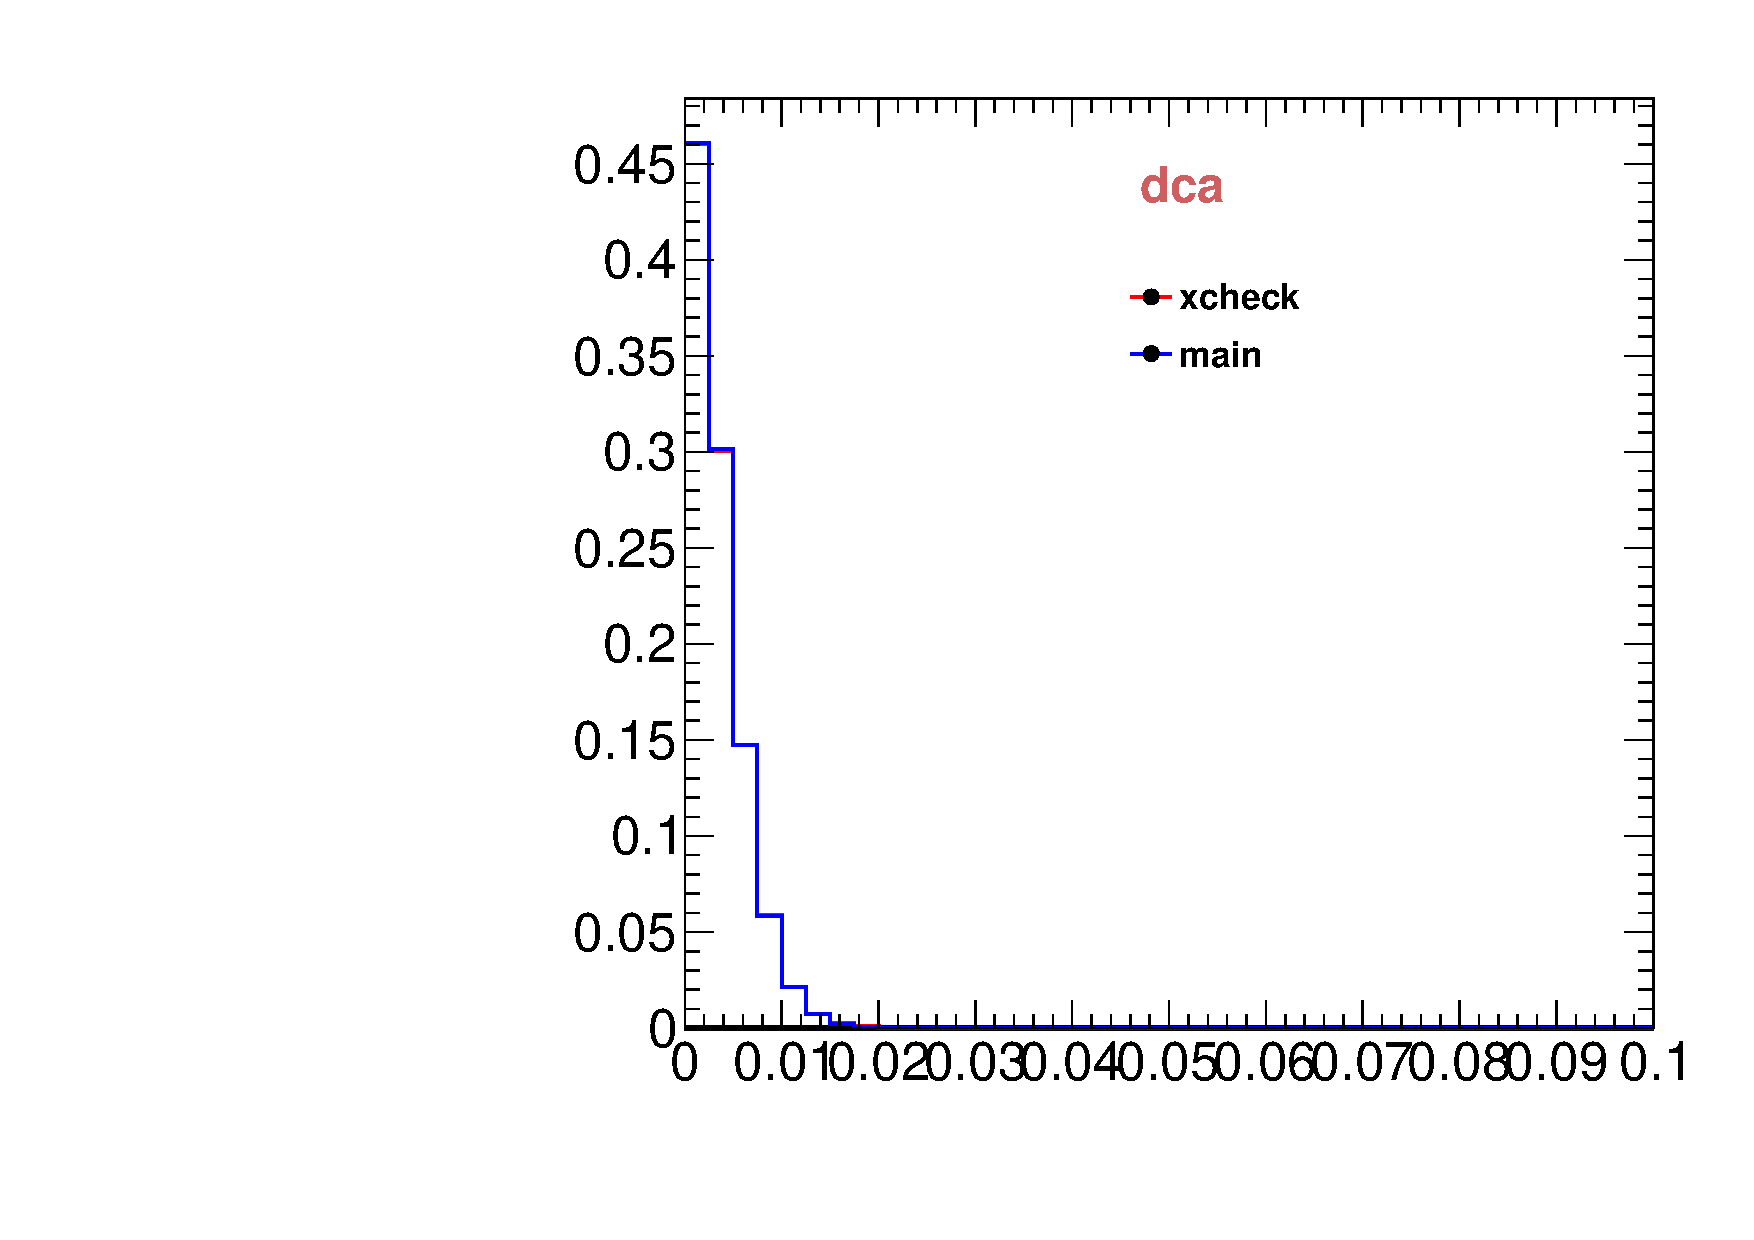
\includegraphics[width=\textwidth]{Figures/VariablesComparison/MC_barrel_figs/maxdoca}
                \label{fig:MC_barrel_maxdoca}
        \end{subfigure}
        \begin{subfigure}[b]{0.2\textwidth}
                \centering
                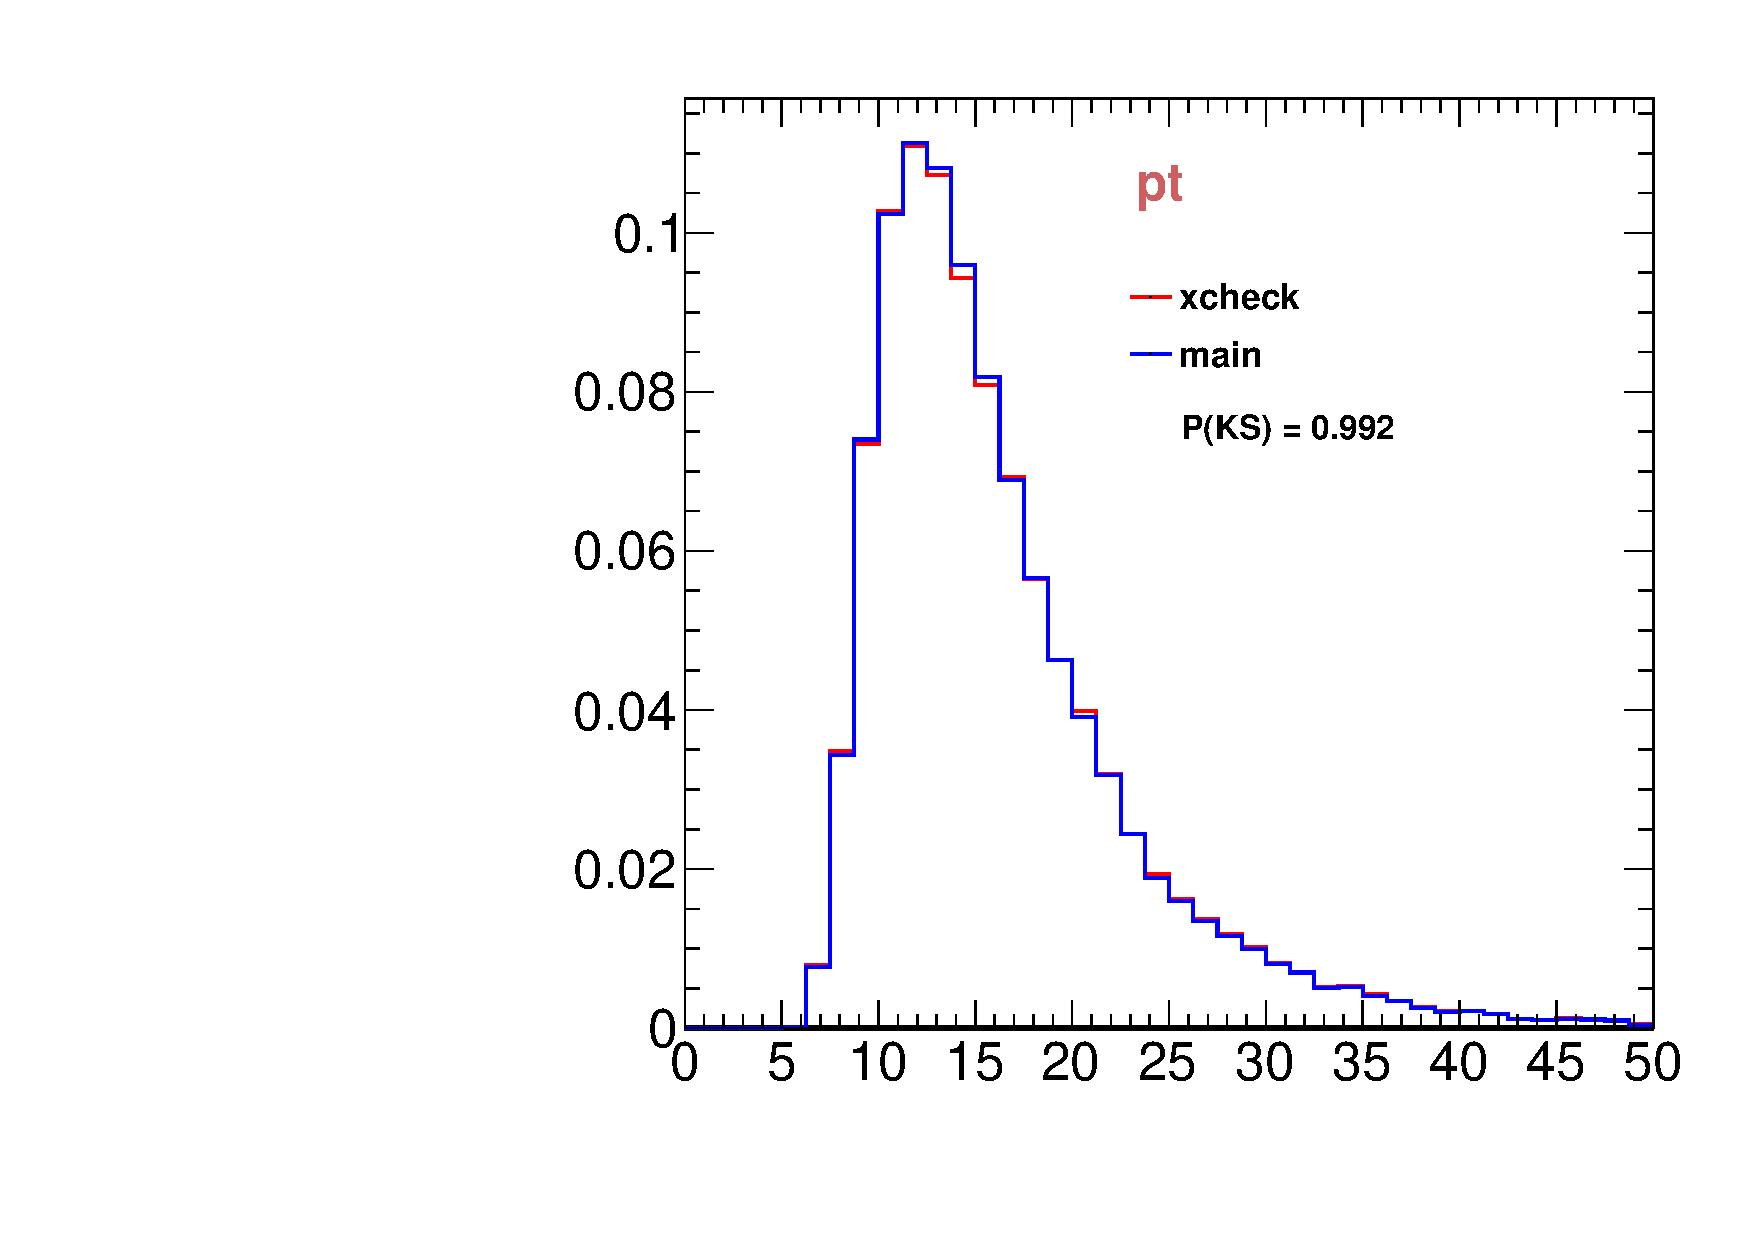
\includegraphics[width=\textwidth]{Figures/VariablesComparison/MC_barrel_figs/pt}
                \label{fig:MC_barrel_pt}
        \end{subfigure}
        \begin{subfigure}[b]{0.2\textwidth}
                \centering
                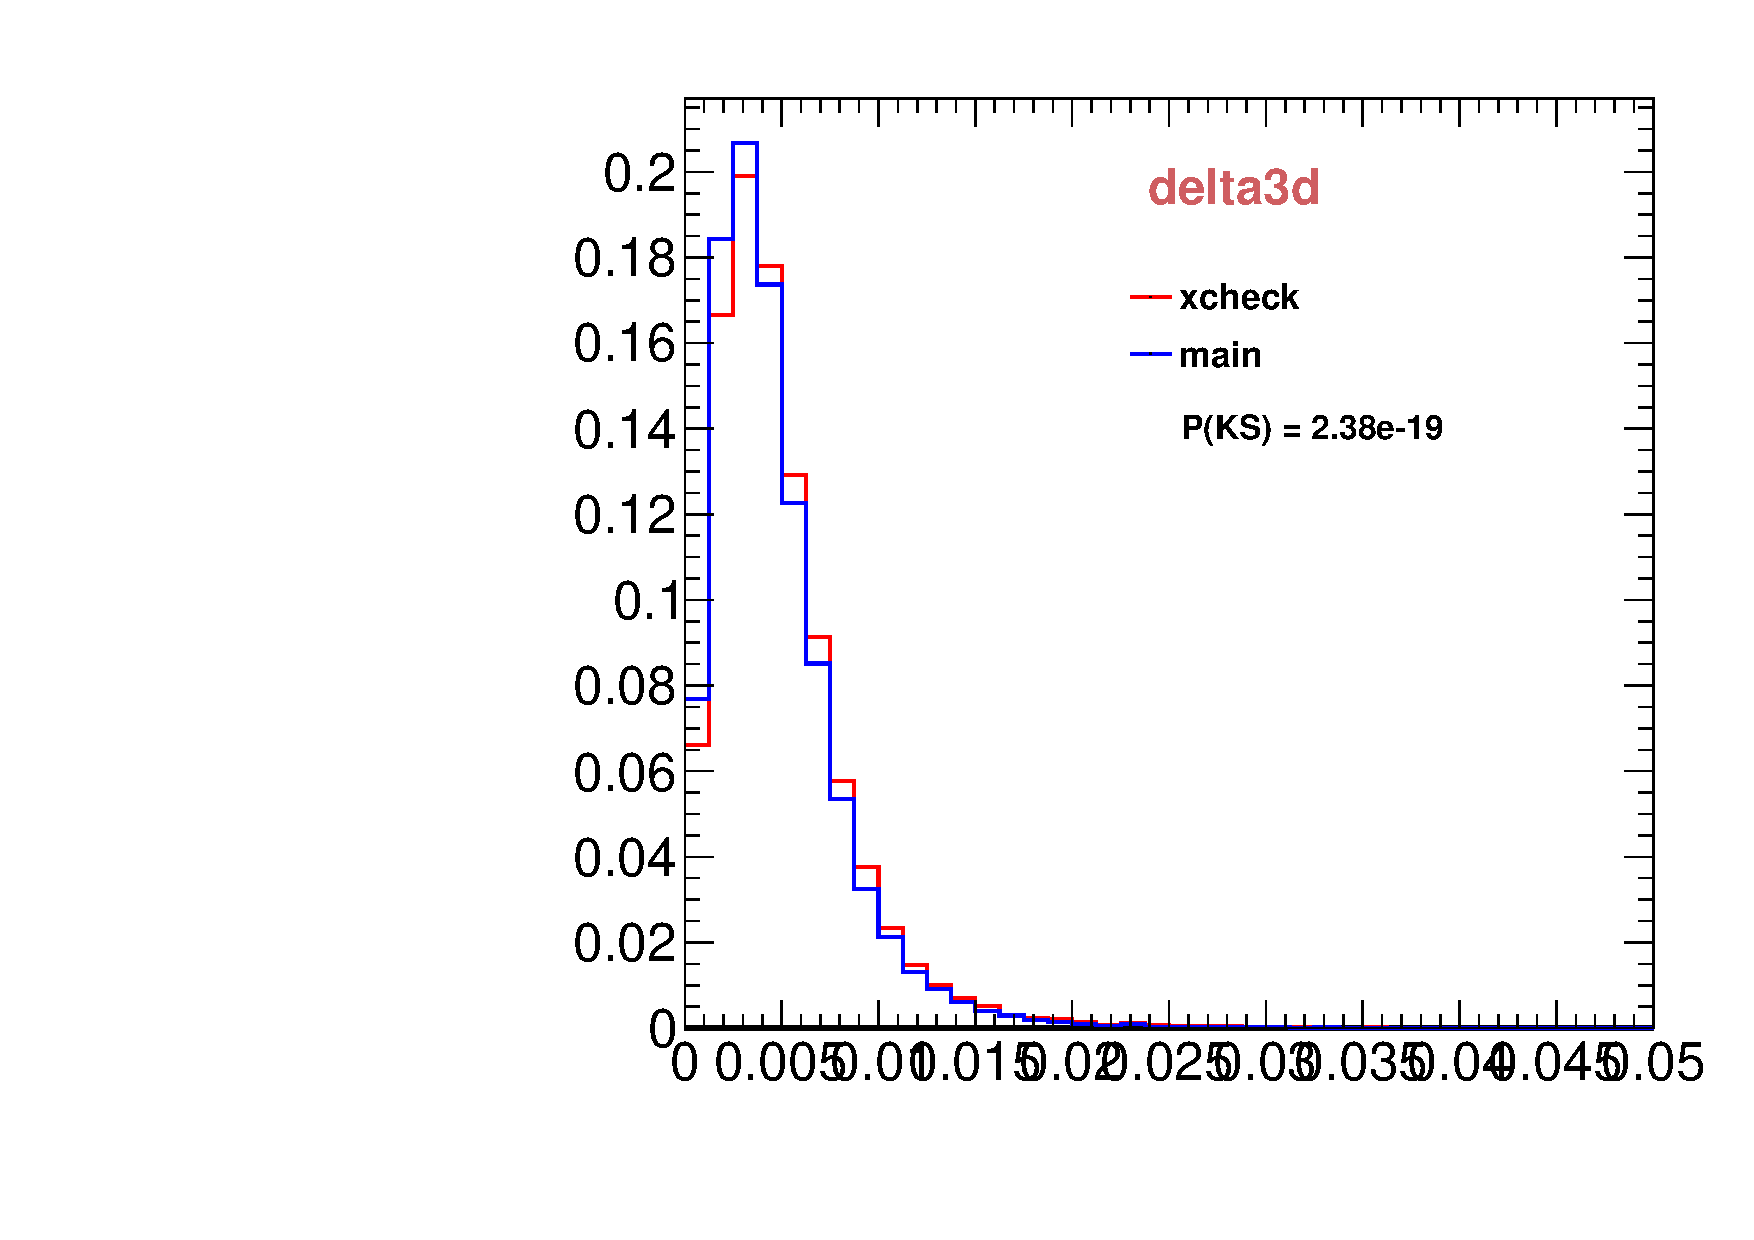
\includegraphics[width=\textwidth]{Figures/VariablesComparison/MC_barrel_figs/pvip}
                \label{fig:MC_barrel_pvip}
        \end{subfigure}
        \begin{subfigure}[b]{0.2\textwidth}
                \centering
                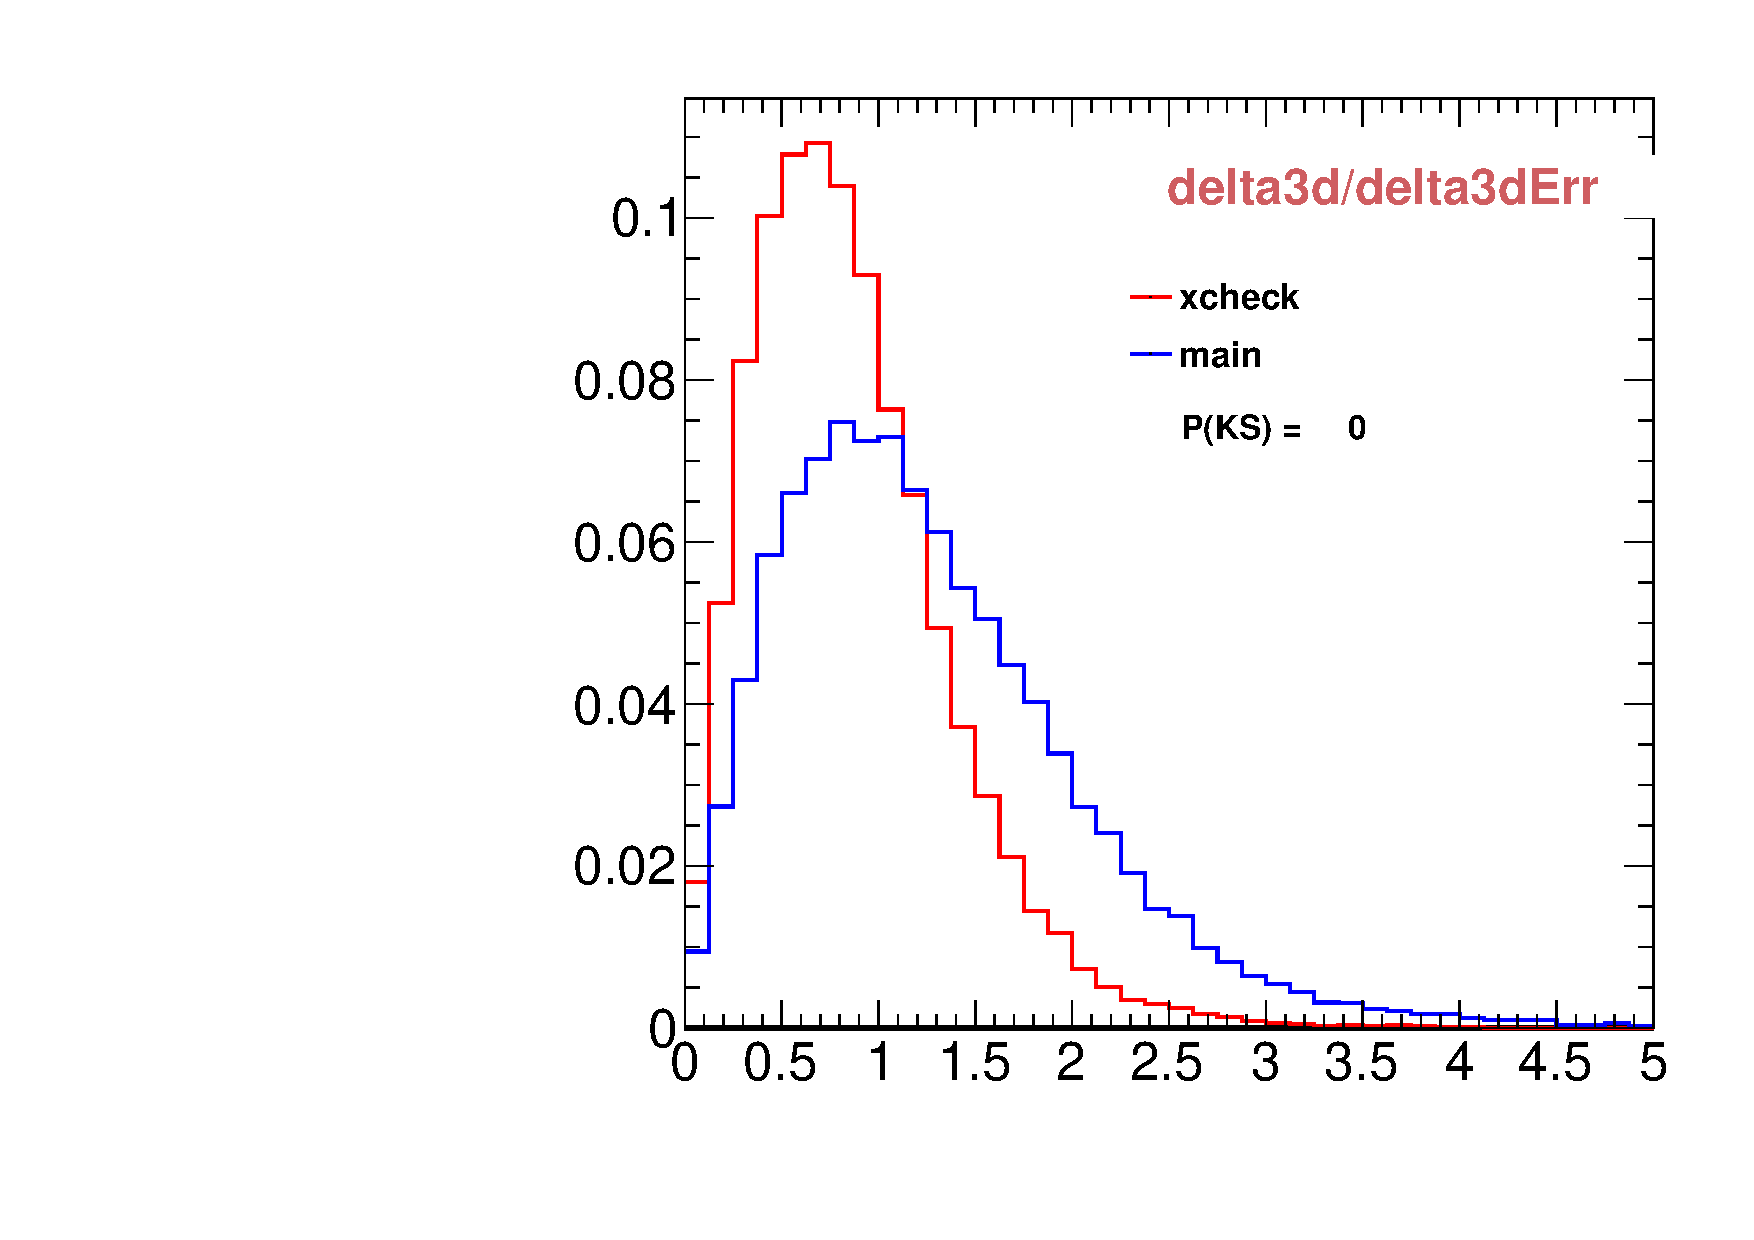
\includegraphics[width=\textwidth]{Figures/VariablesComparison/MC_barrel_figs/pvips}
                \label{fig:MC_barrel_pvips}
        \end{subfigure}
        \begin{subfigure}[b]{0.2\textwidth}
                \centering
                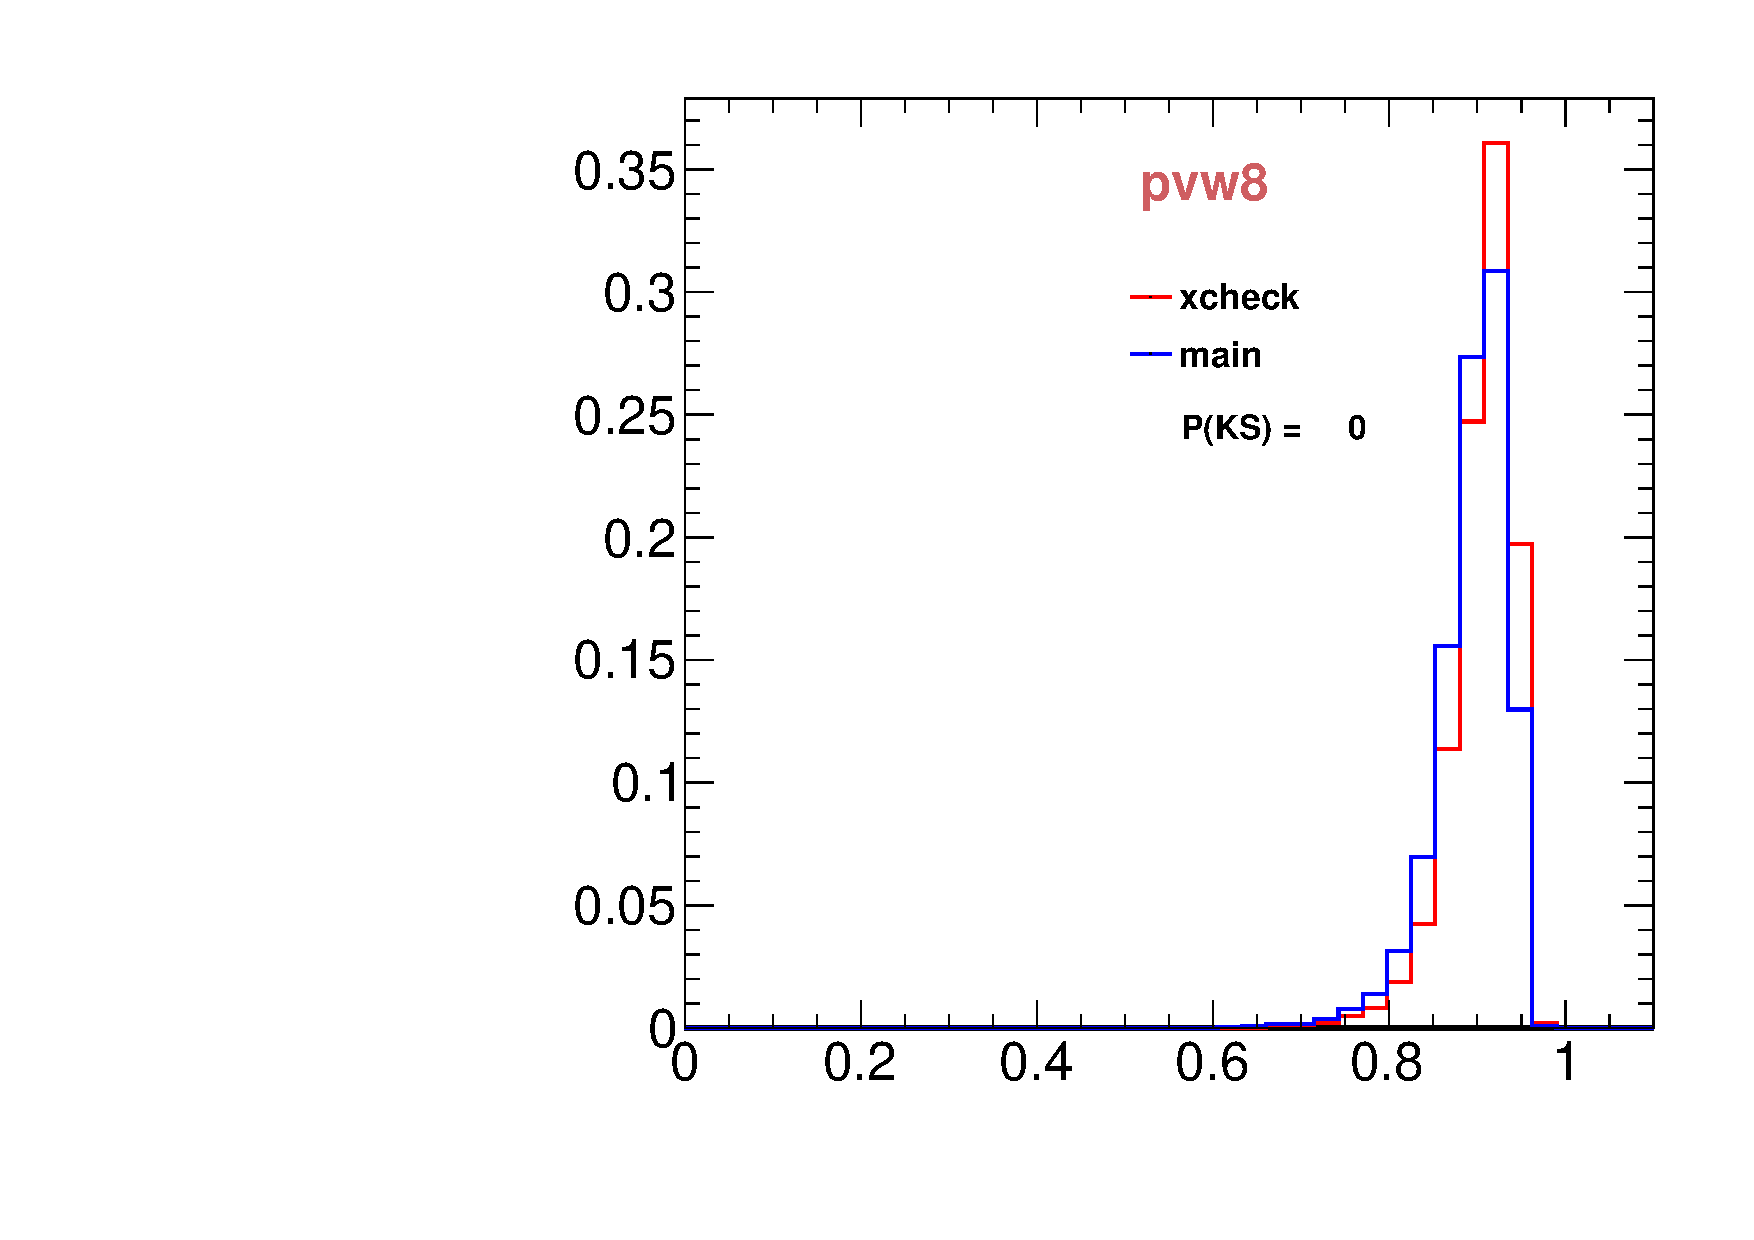
\includegraphics[width=\textwidth]{Figures/VariablesComparison/MC_barrel_figs/pvw8}
                \label{fig:MC_barrel_pvw8}
        \end{subfigure}
        \caption{Variable comparisons between the main analysis and the cross-check analysis. Part I: MC barrel.}
        \label{fig:MC_barrel_figs}
\end{sidewaysfigure}


\begin{sidewaysfigure}
        \centering
        \begin{subfigure}[b]{0.2\textwidth}
                \centering
                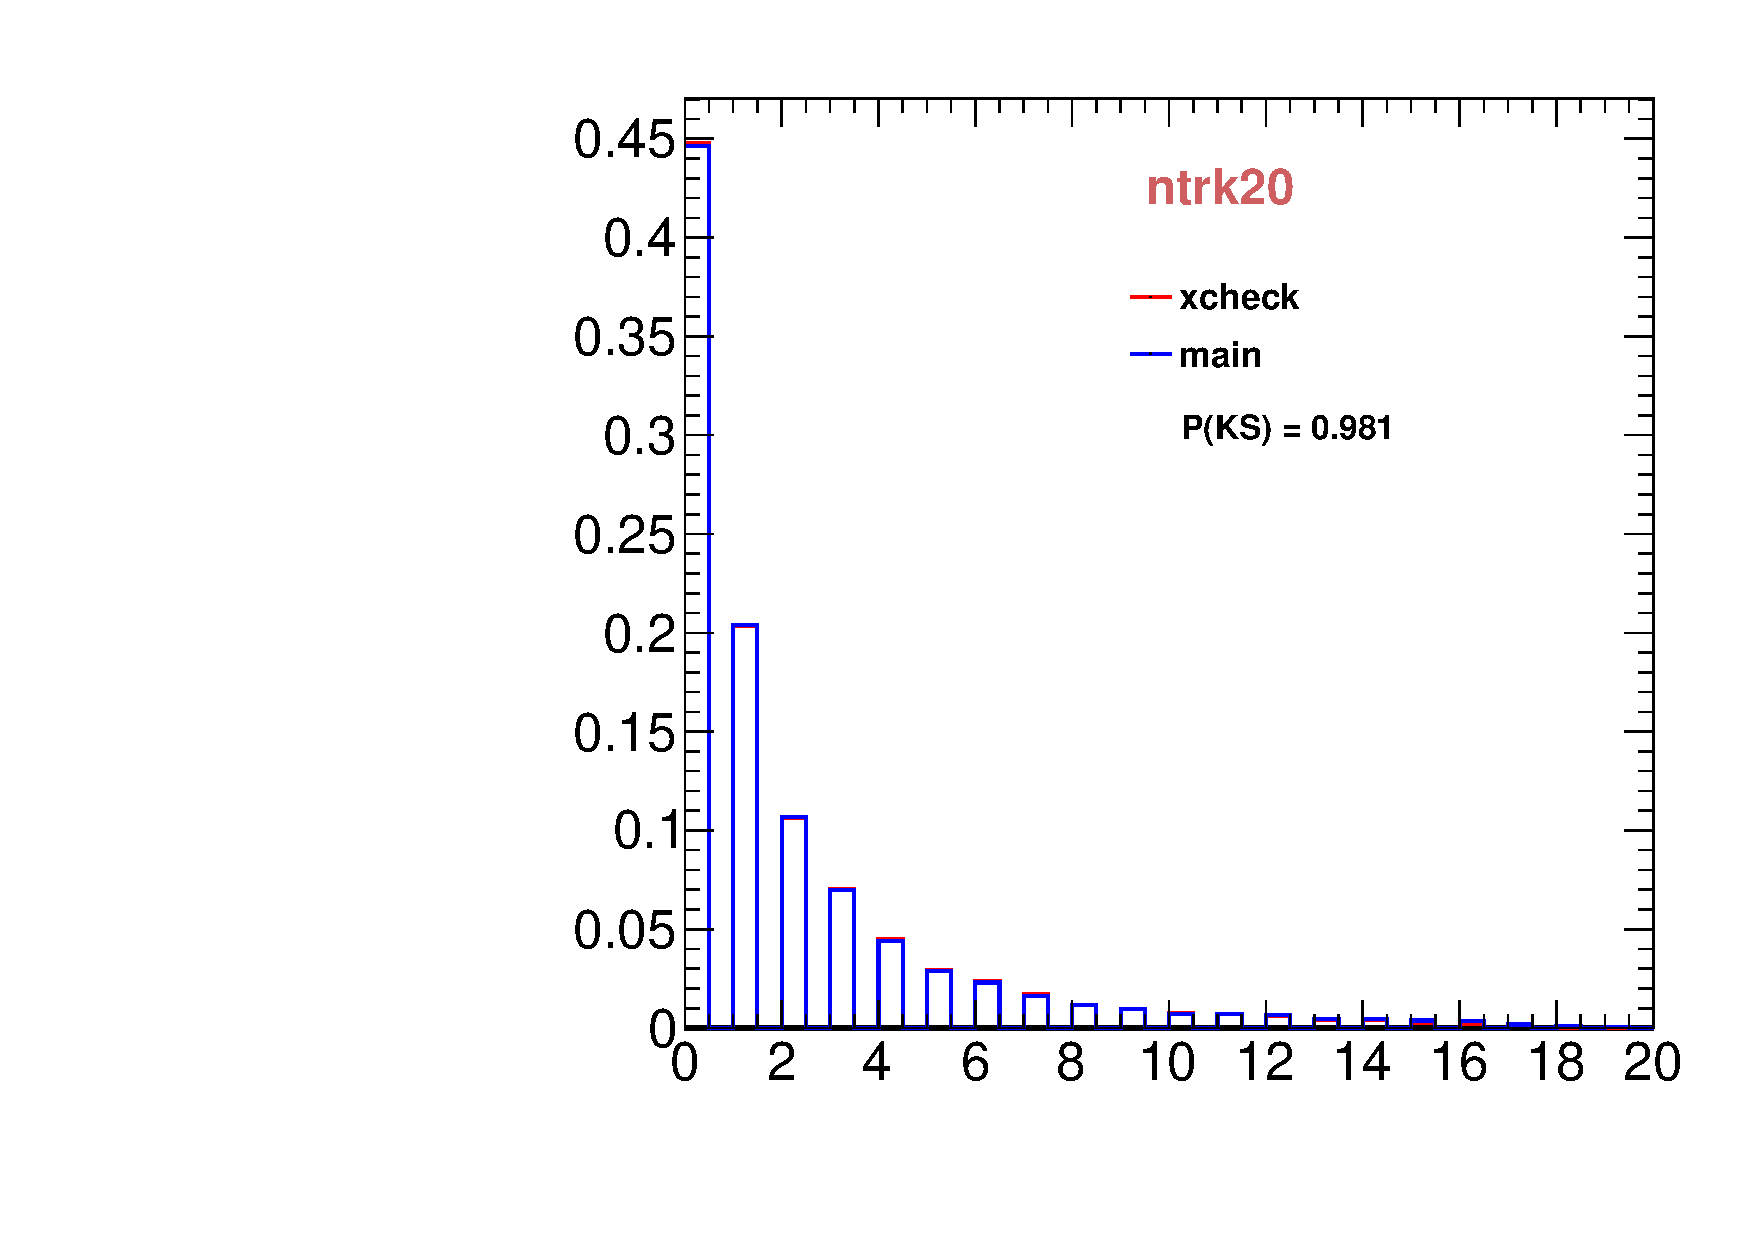
\includegraphics[width=\textwidth]{Figures/VariablesComparison/MC_endcaps_figs/closetrk}
                \label{fig:MC_endcaps_closetrk}
        \end{subfigure}
        \begin{subfigure}[b]{0.2\textwidth}
                \centering
                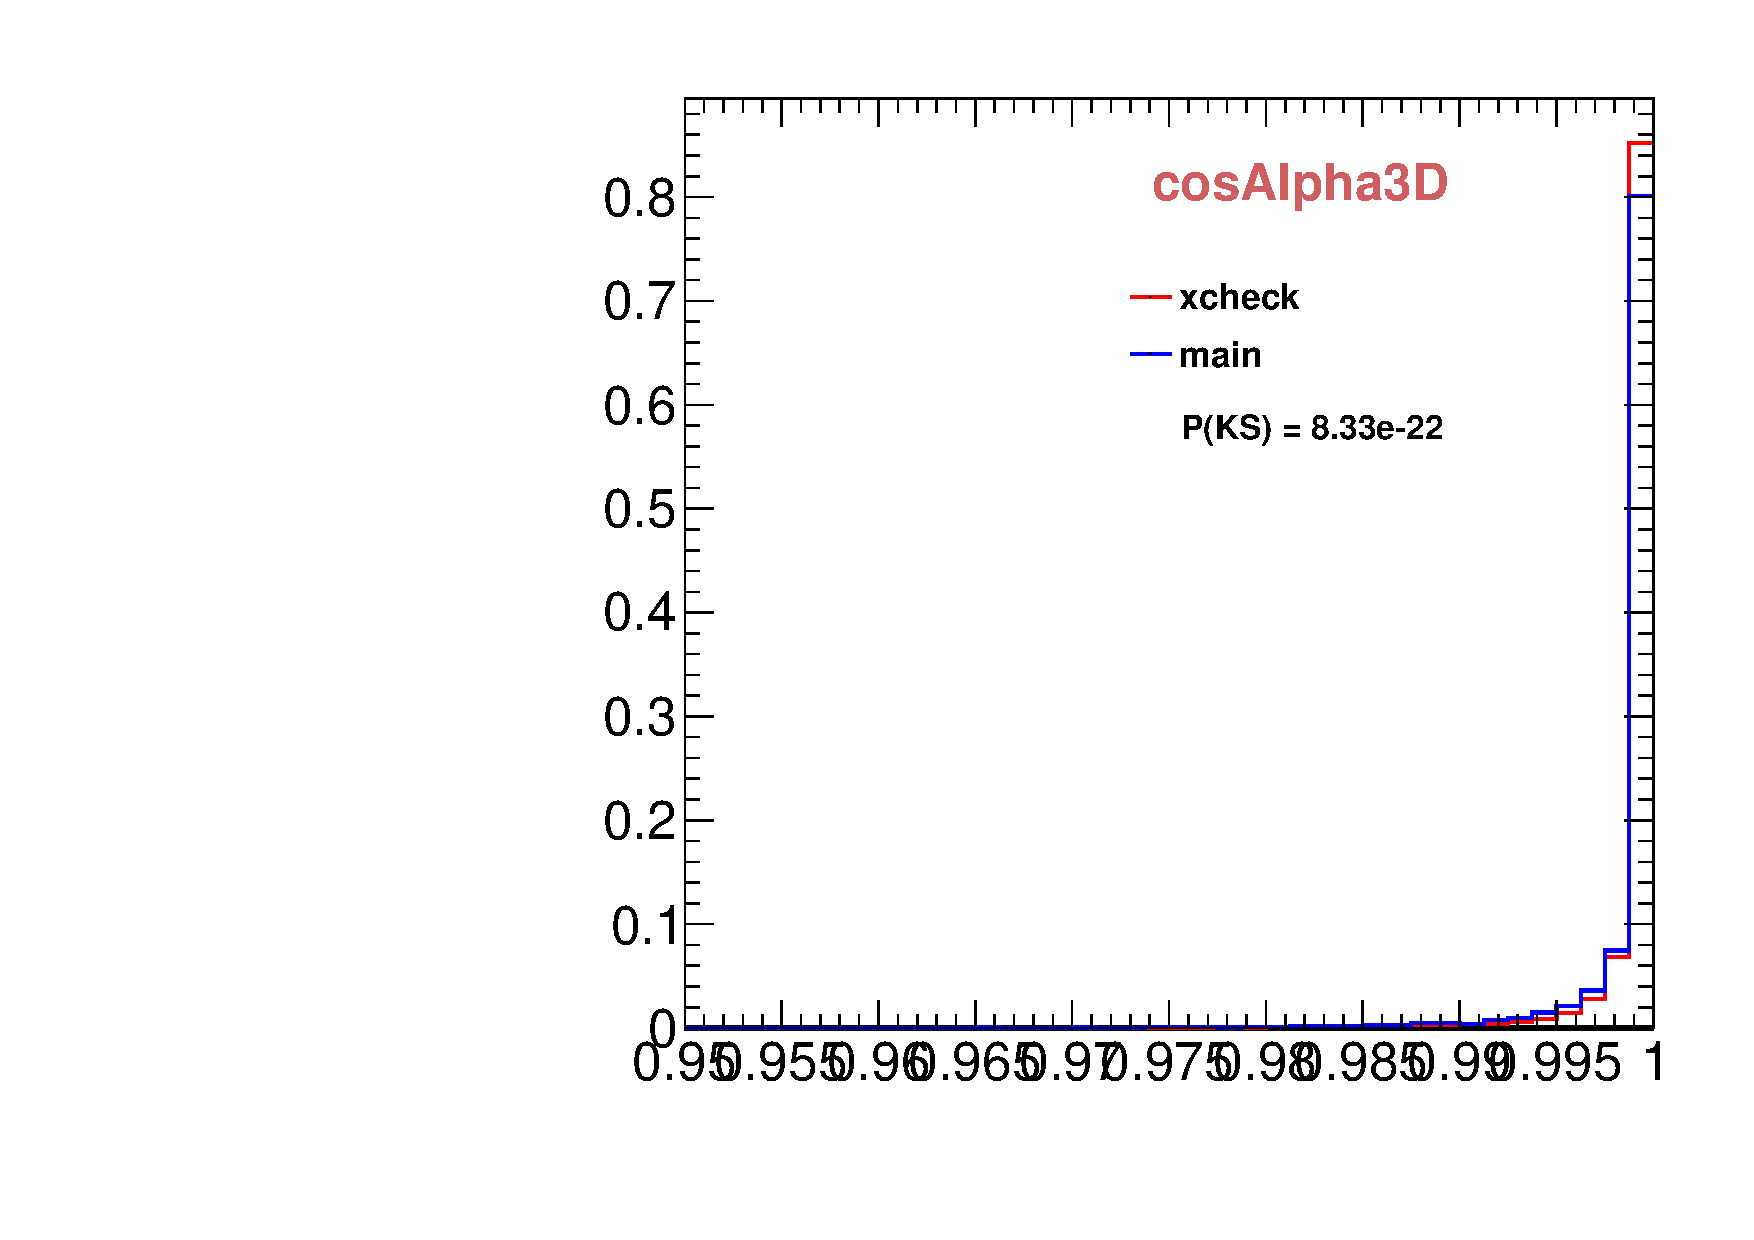
\includegraphics[width=\textwidth]{Figures/VariablesComparison/MC_endcaps_figs/cosa}
                \label{fig:MC_endcaps_cosa}
        \end{subfigure}
        \begin{subfigure}[b]{0.2\textwidth}
                \centering
                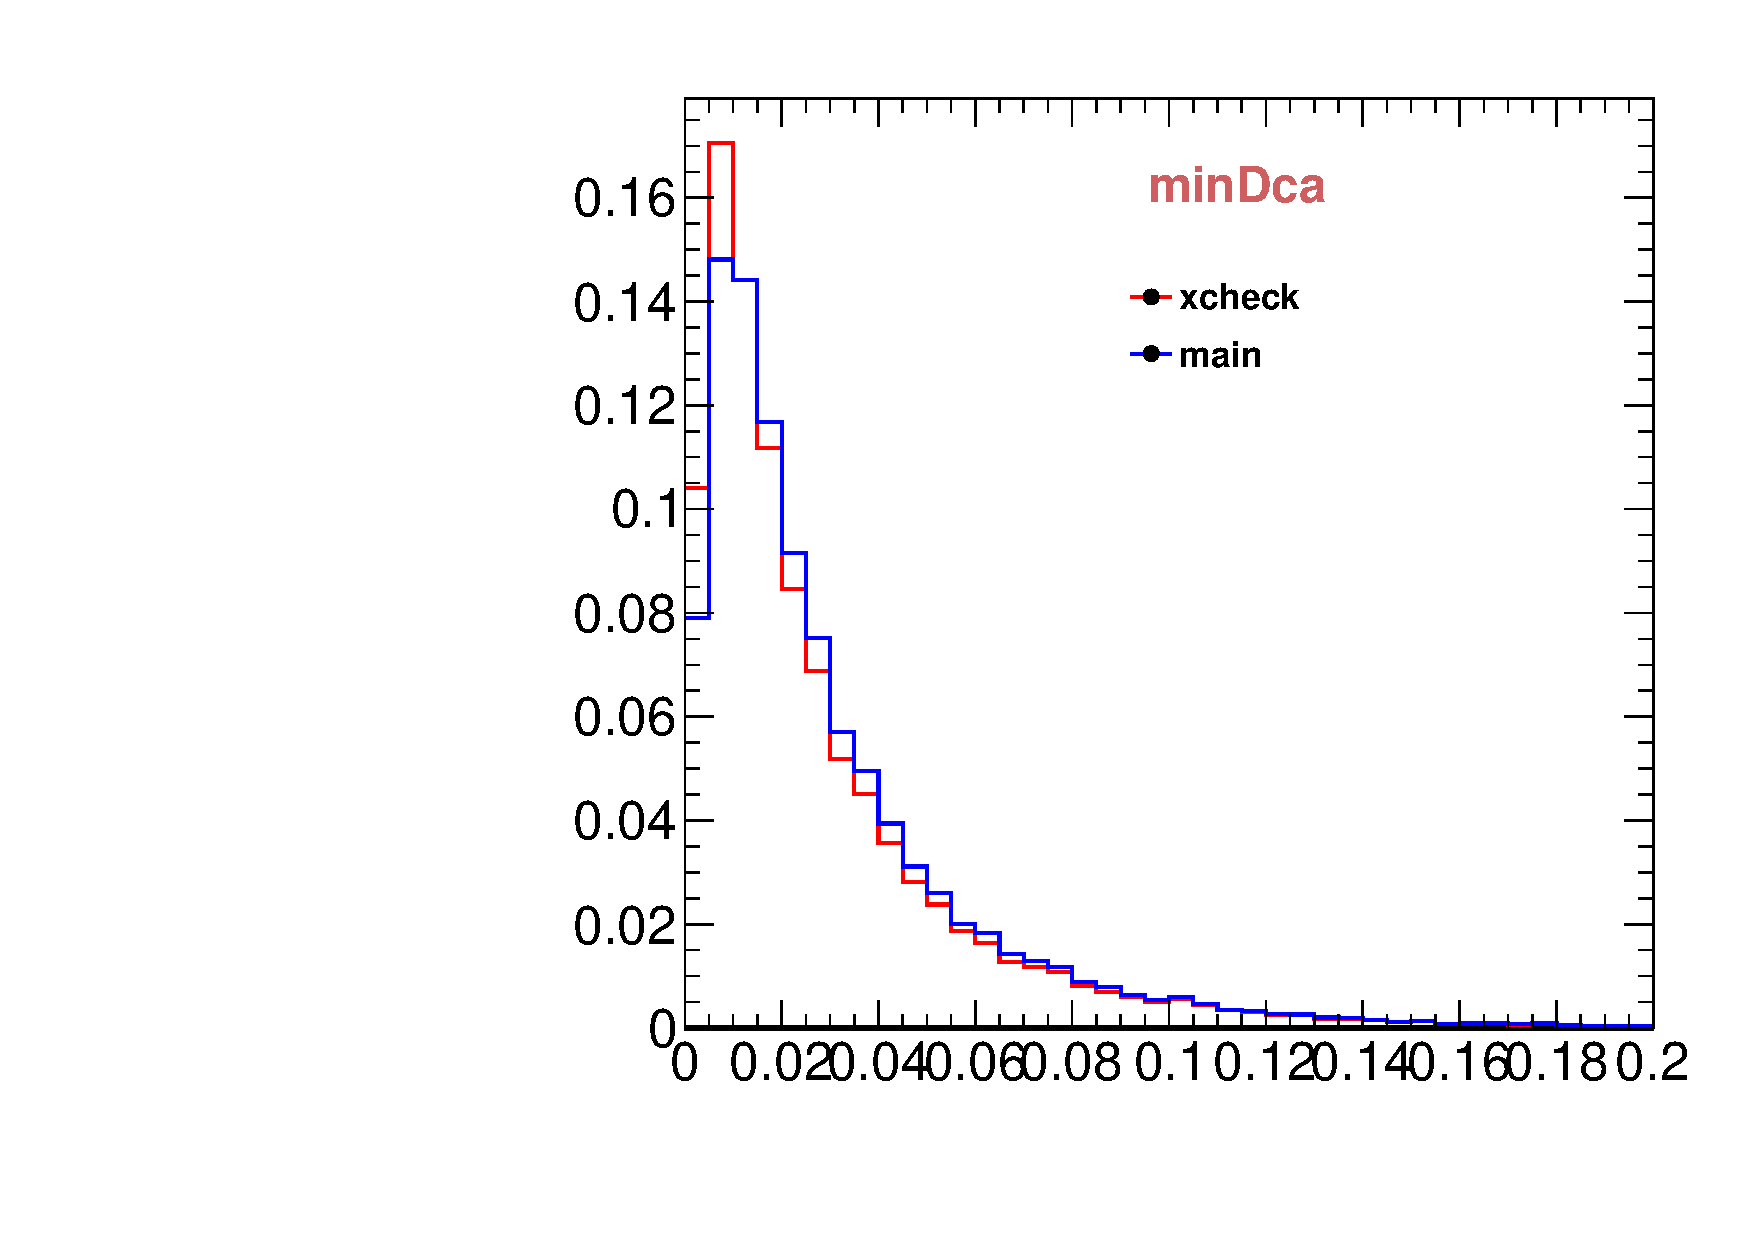
\includegraphics[width=\textwidth]{Figures/VariablesComparison/MC_endcaps_figs/docatrk}
                \label{fig:MC_endcaps_docatrk}
        \end{subfigure}
        \begin{subfigure}[b]{0.2\textwidth}
                \centering
                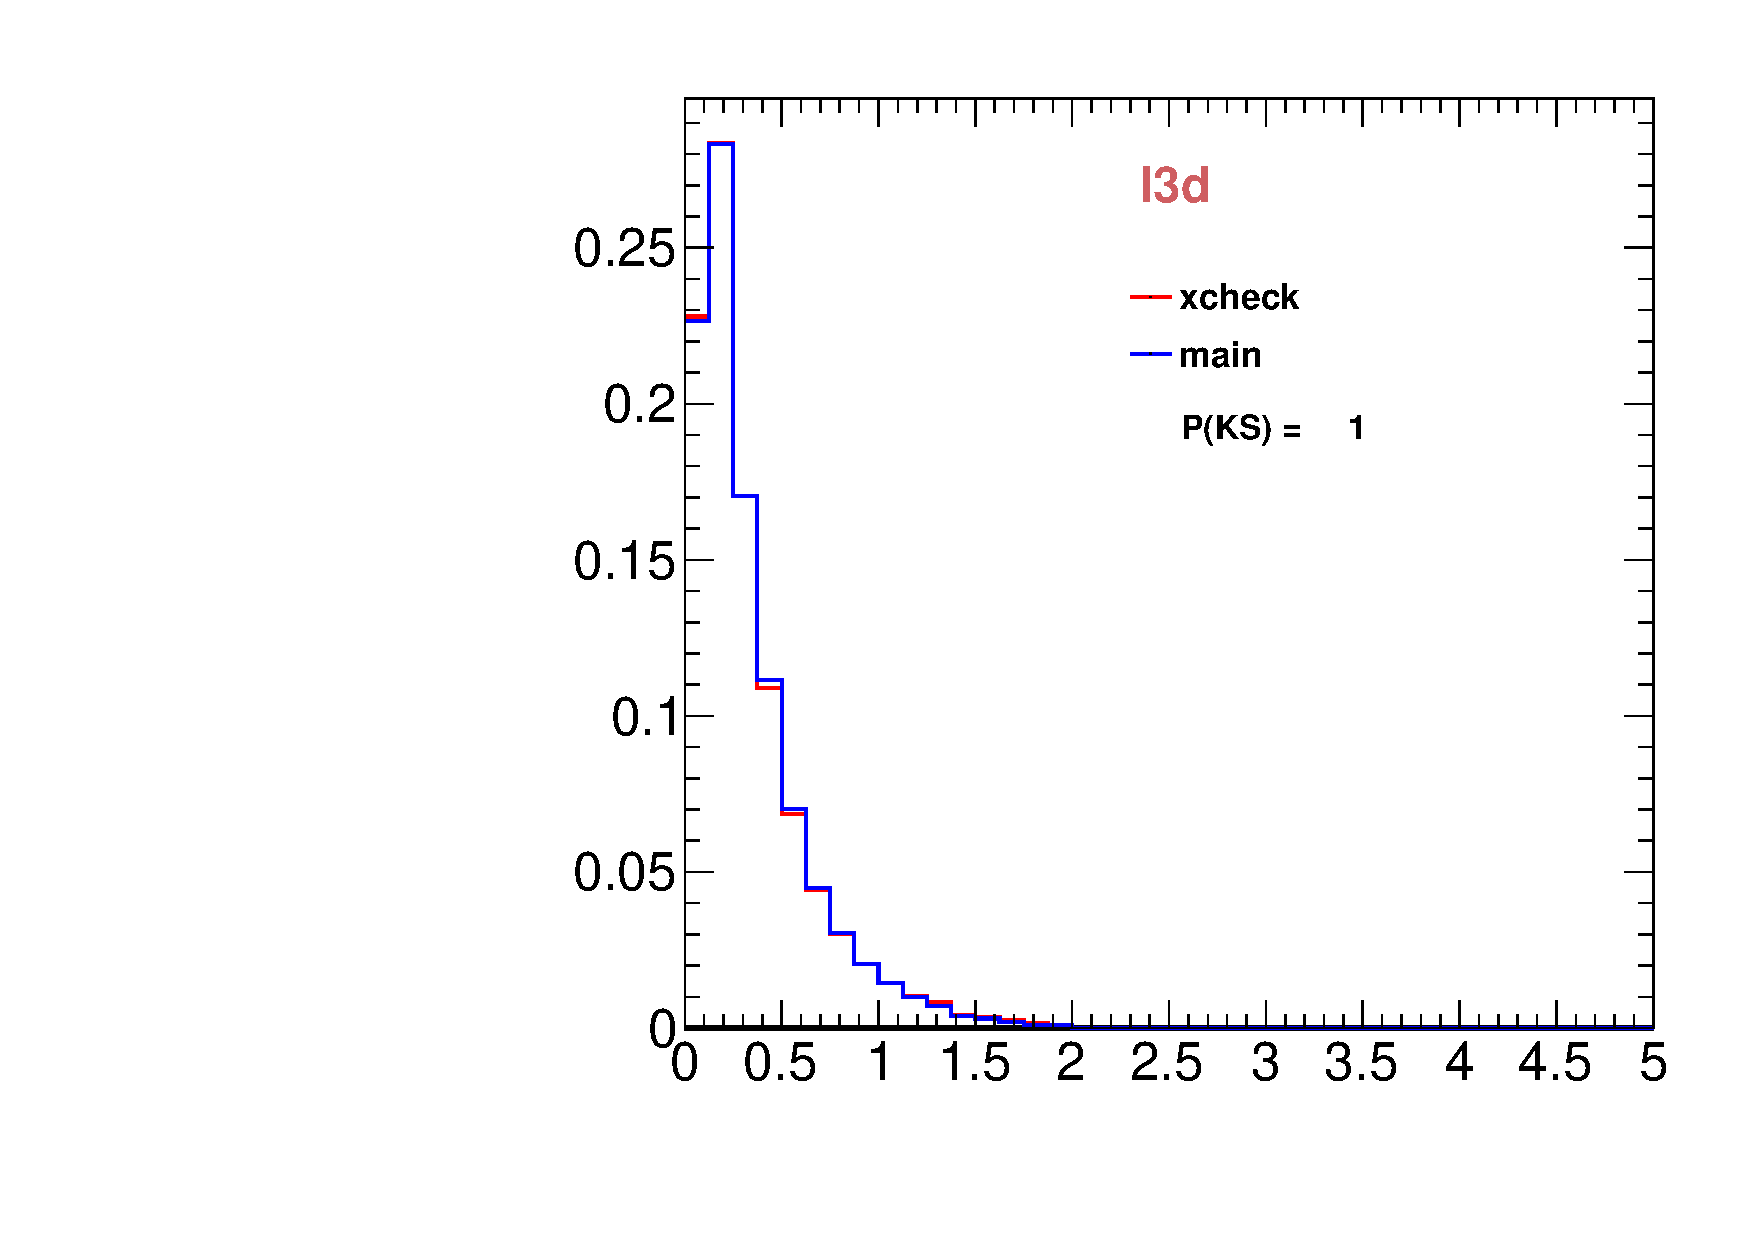
\includegraphics[width=\textwidth]{Figures/VariablesComparison/MC_endcaps_figs/fl3d}
                \label{fig:MC_endcaps_fl3d}
        \end{subfigure}
        \begin{subfigure}[b]{0.2\textwidth}
                \centering
                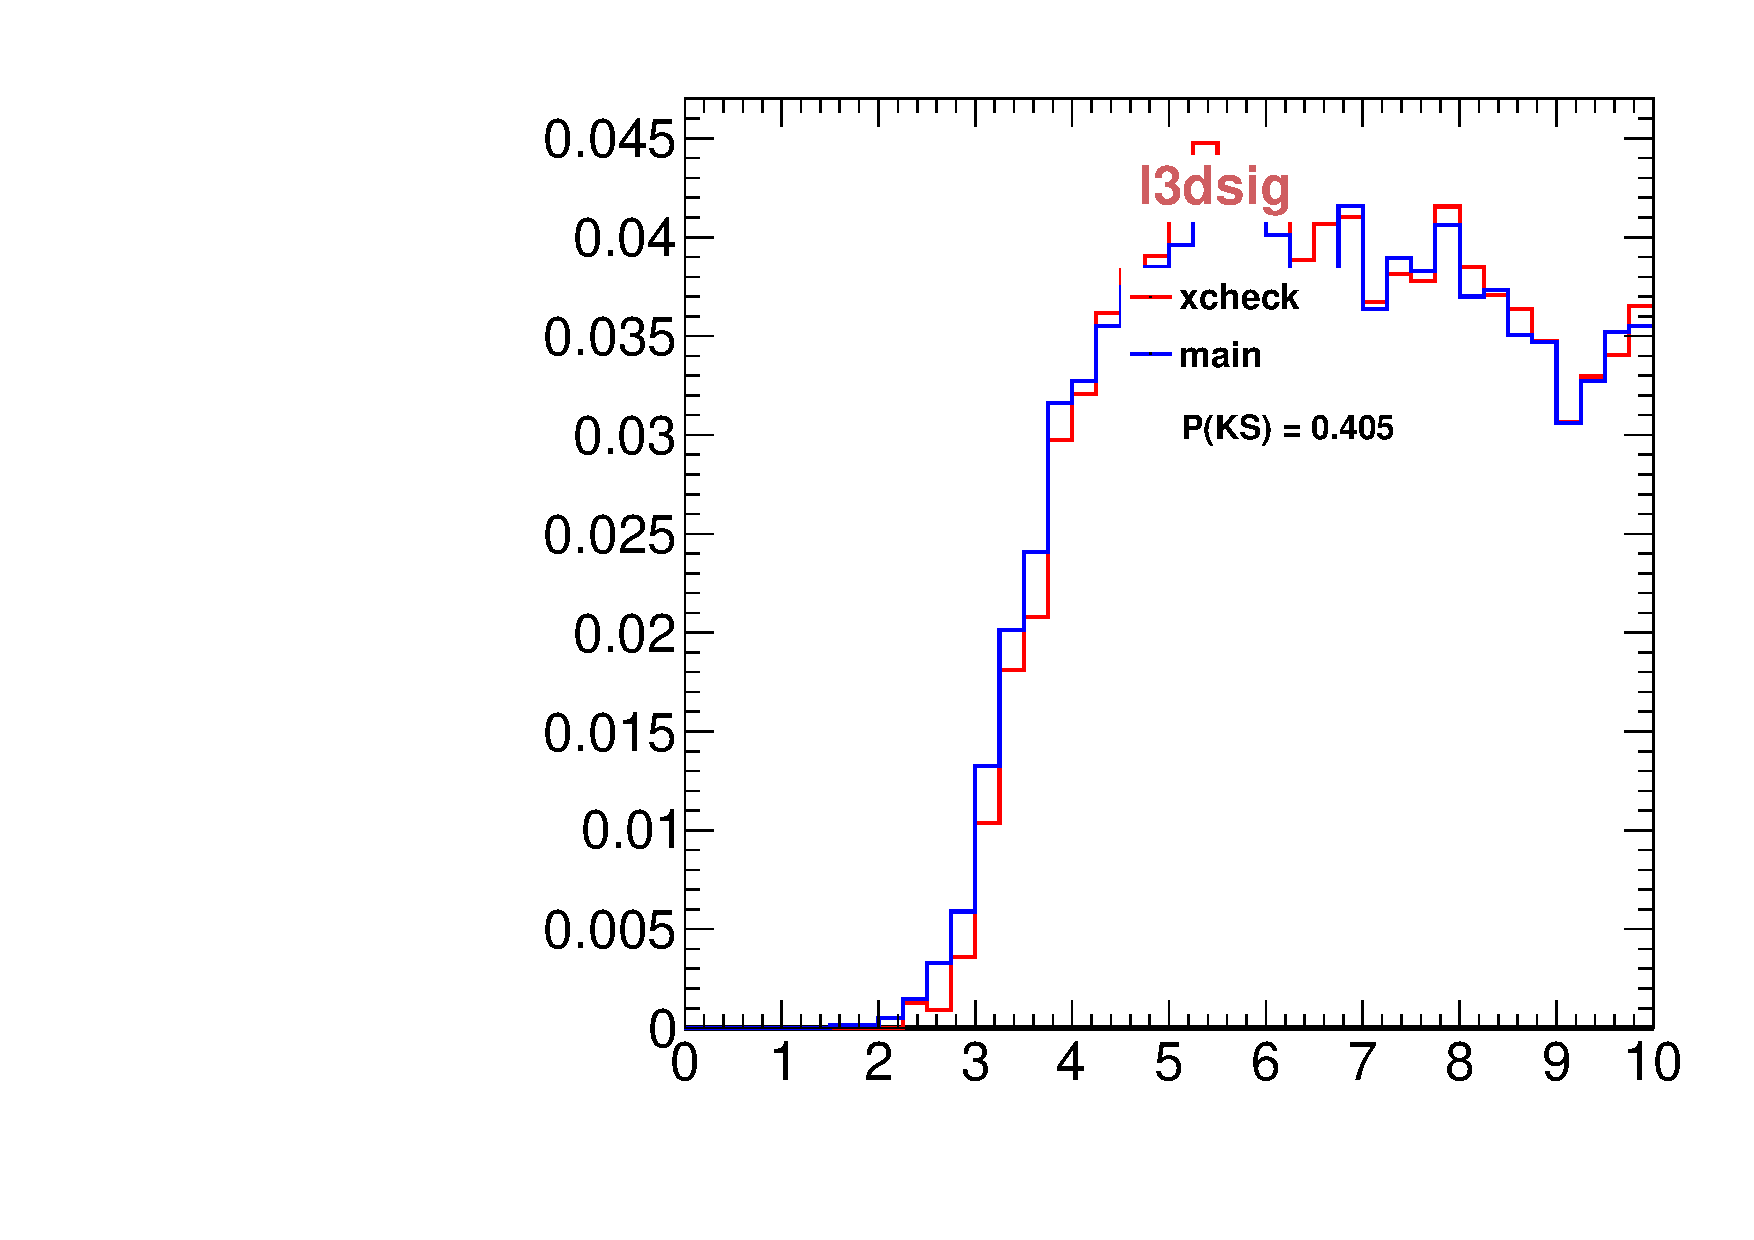
\includegraphics[width=\textwidth]{Figures/VariablesComparison/MC_endcaps_figs/fls3d}
                \label{fig:MC_endcaps_fls3d}
        \end{subfigure}
        \begin{subfigure}[b]{0.2\textwidth}
                \centering
                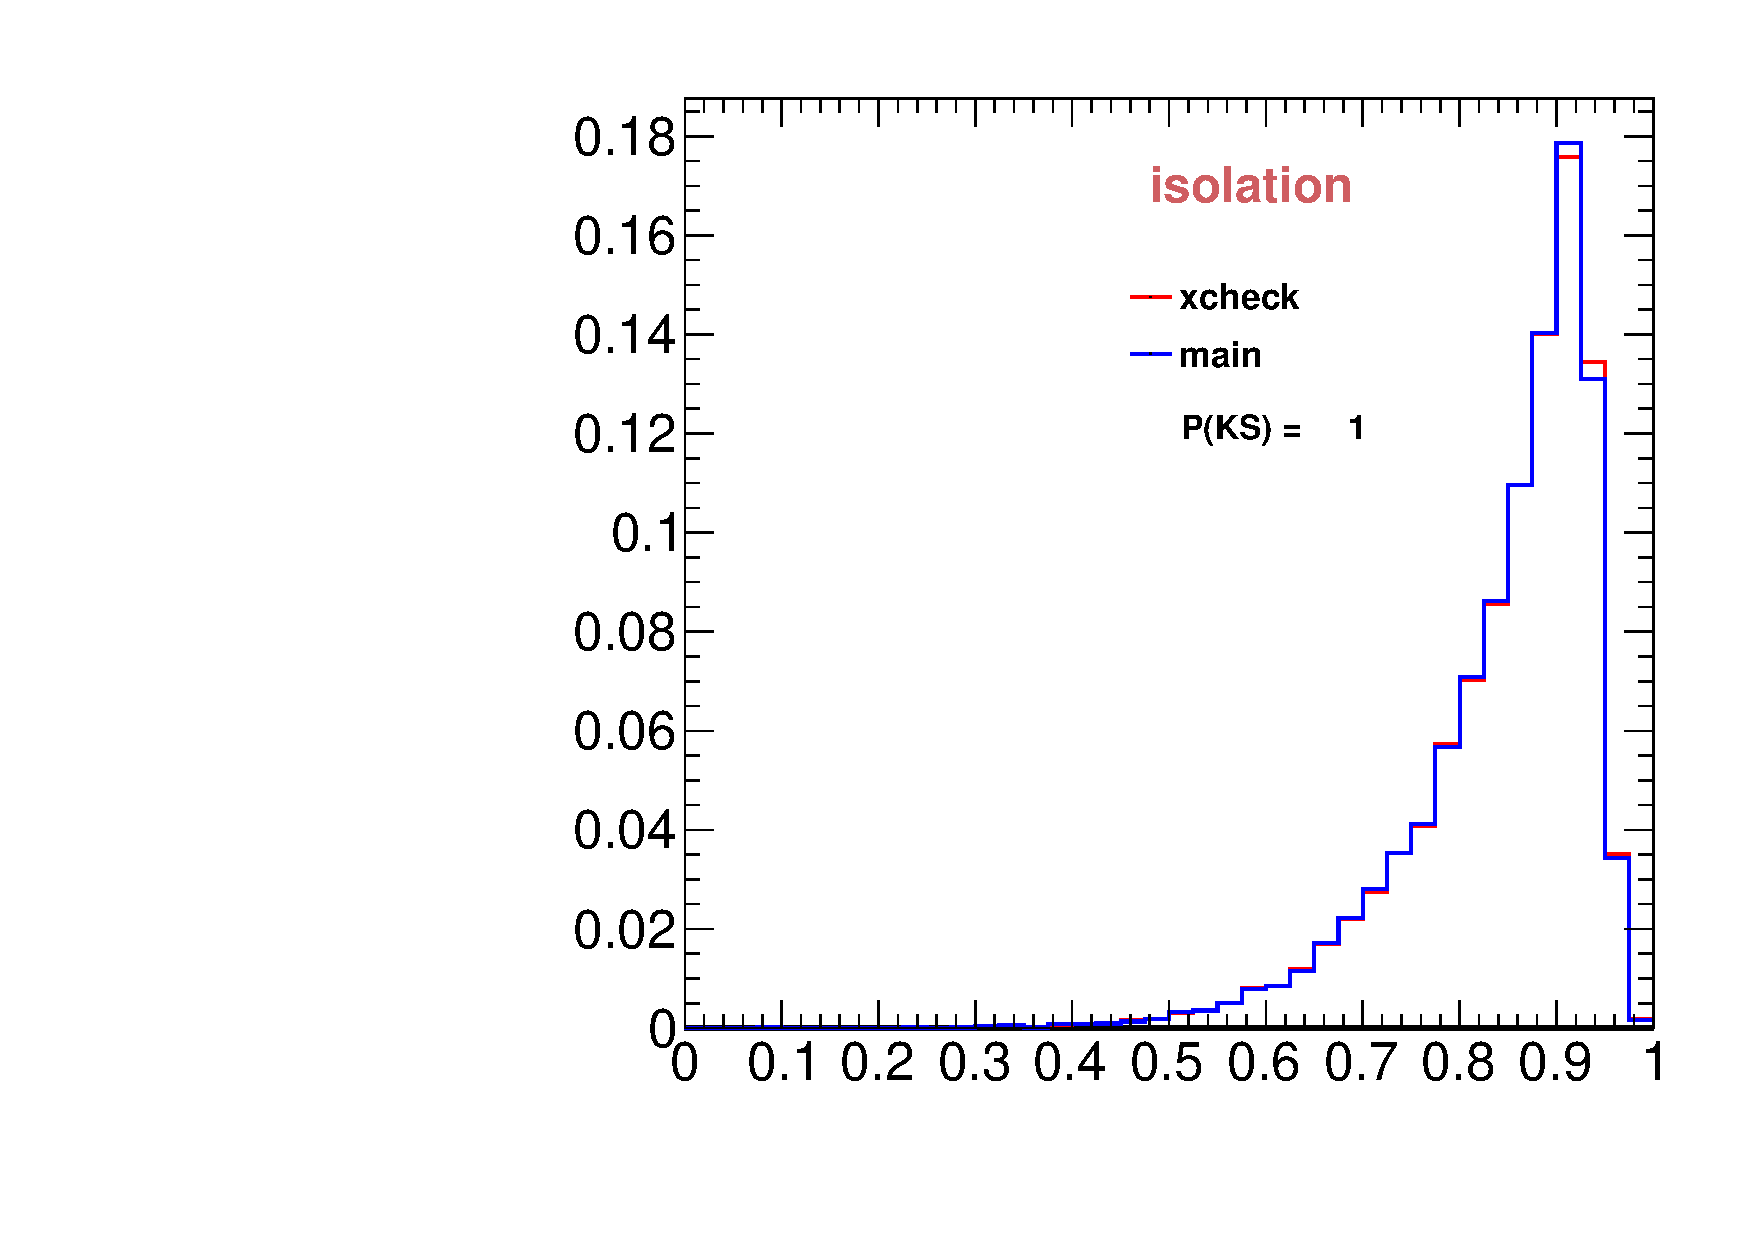
\includegraphics[width=\textwidth]{Figures/VariablesComparison/MC_endcaps_figs/iso}
                \label{fig:MC_endcaps_iso}
        \end{subfigure}
        \begin{subfigure}[b]{0.2\textwidth}
                \centering
                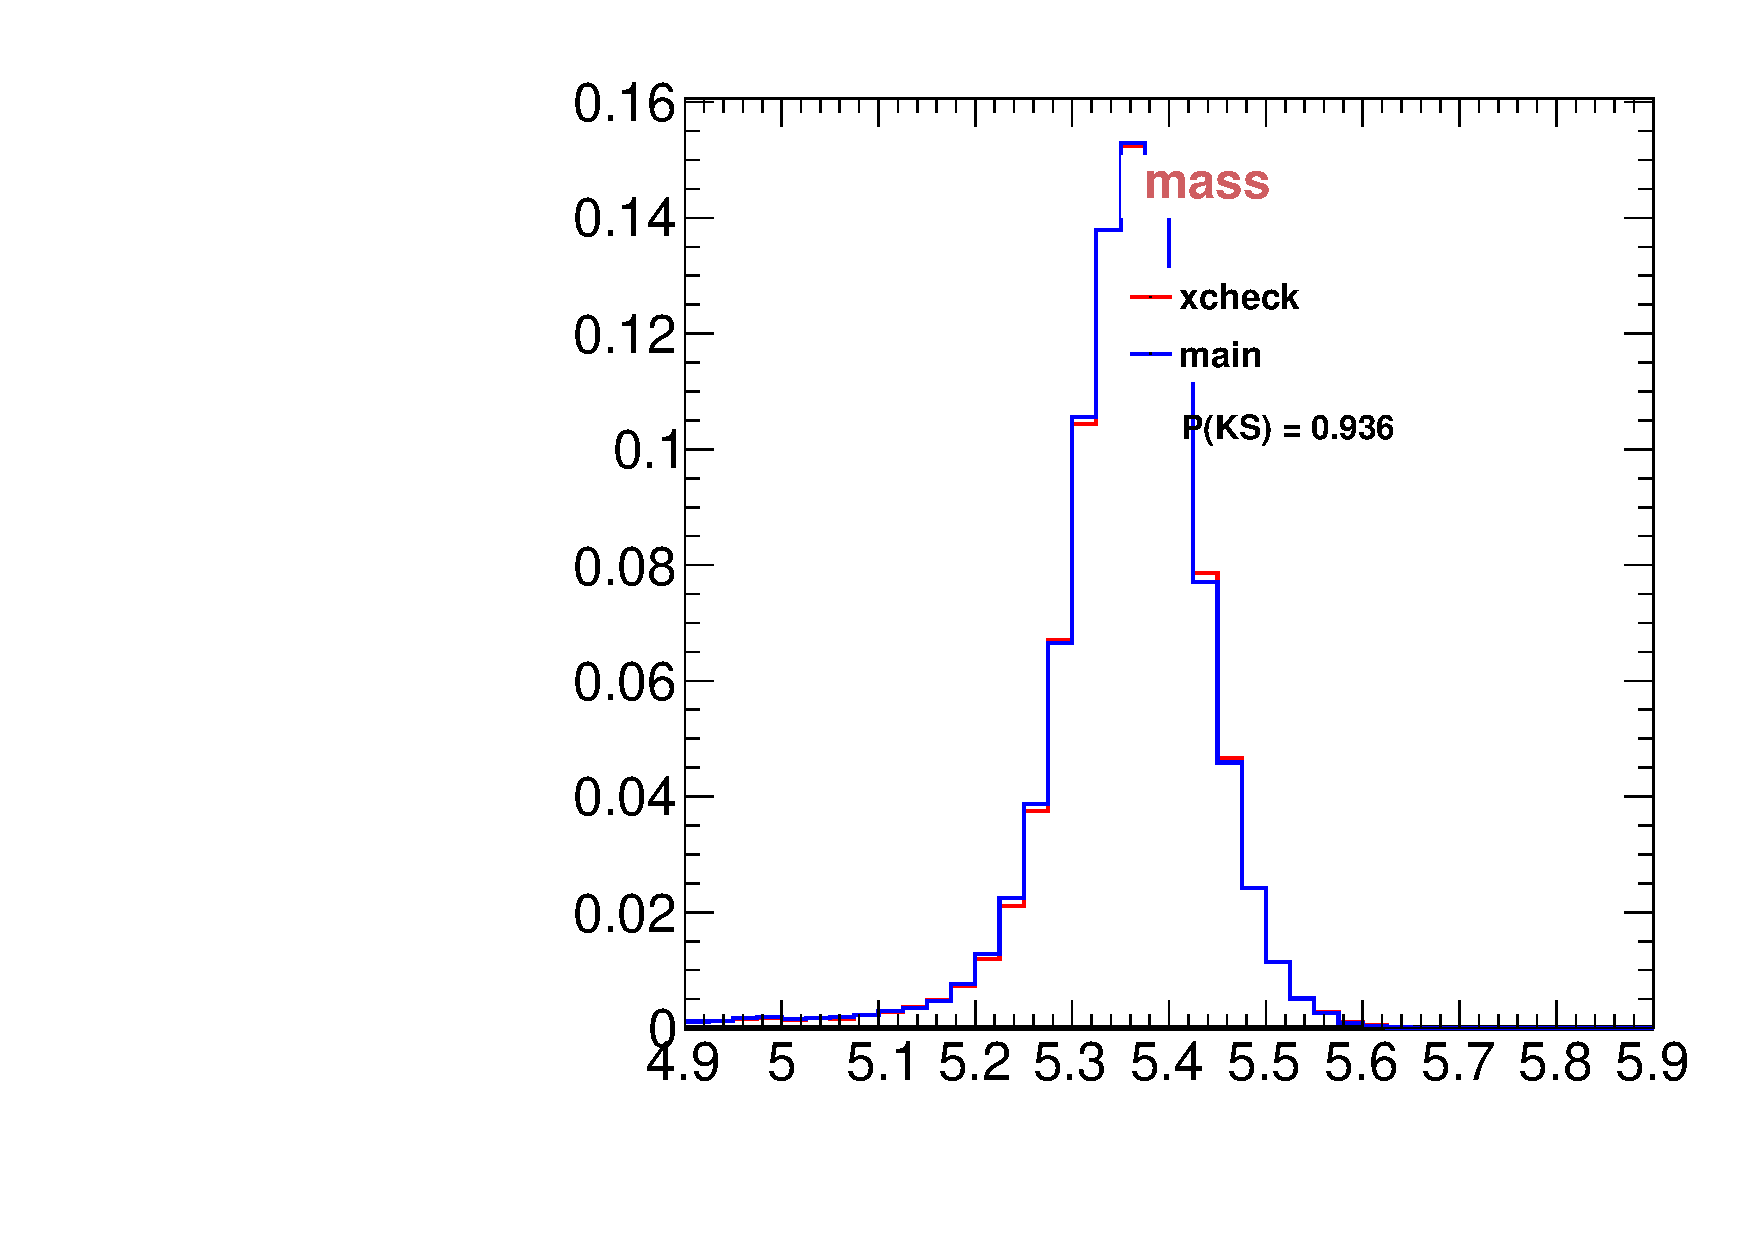
\includegraphics[width=\textwidth]{Figures/VariablesComparison/MC_endcaps_figs/m}
                \label{fig:MC_endcaps_m}
        \end{subfigure}
        \begin{subfigure}[b]{0.2\textwidth}
                \centering
                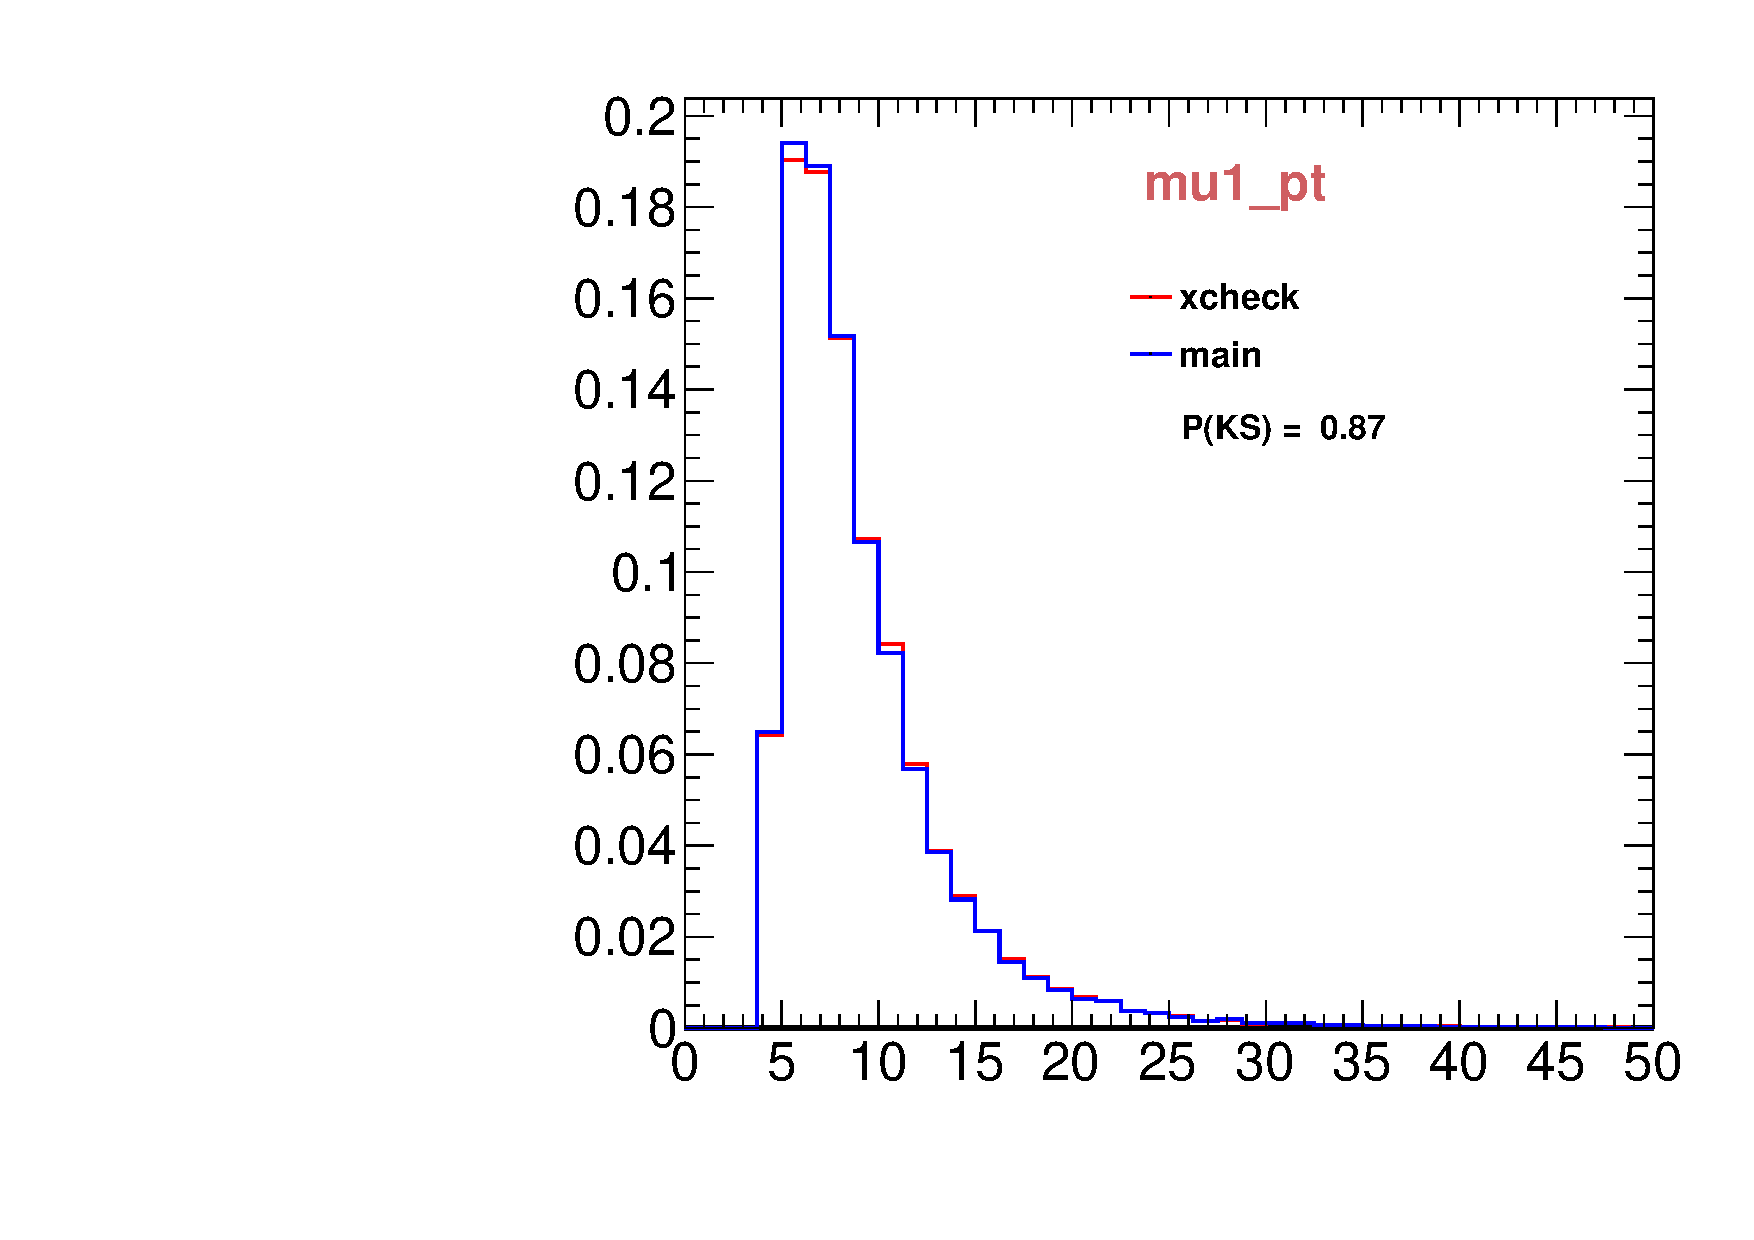
\includegraphics[width=\textwidth]{Figures/VariablesComparison/MC_endcaps_figs/m1pt}
                \label{fig:MC_endcaps_m1pt}
        \end{subfigure}
        \begin{subfigure}[b]{0.2\textwidth}
                \centering
                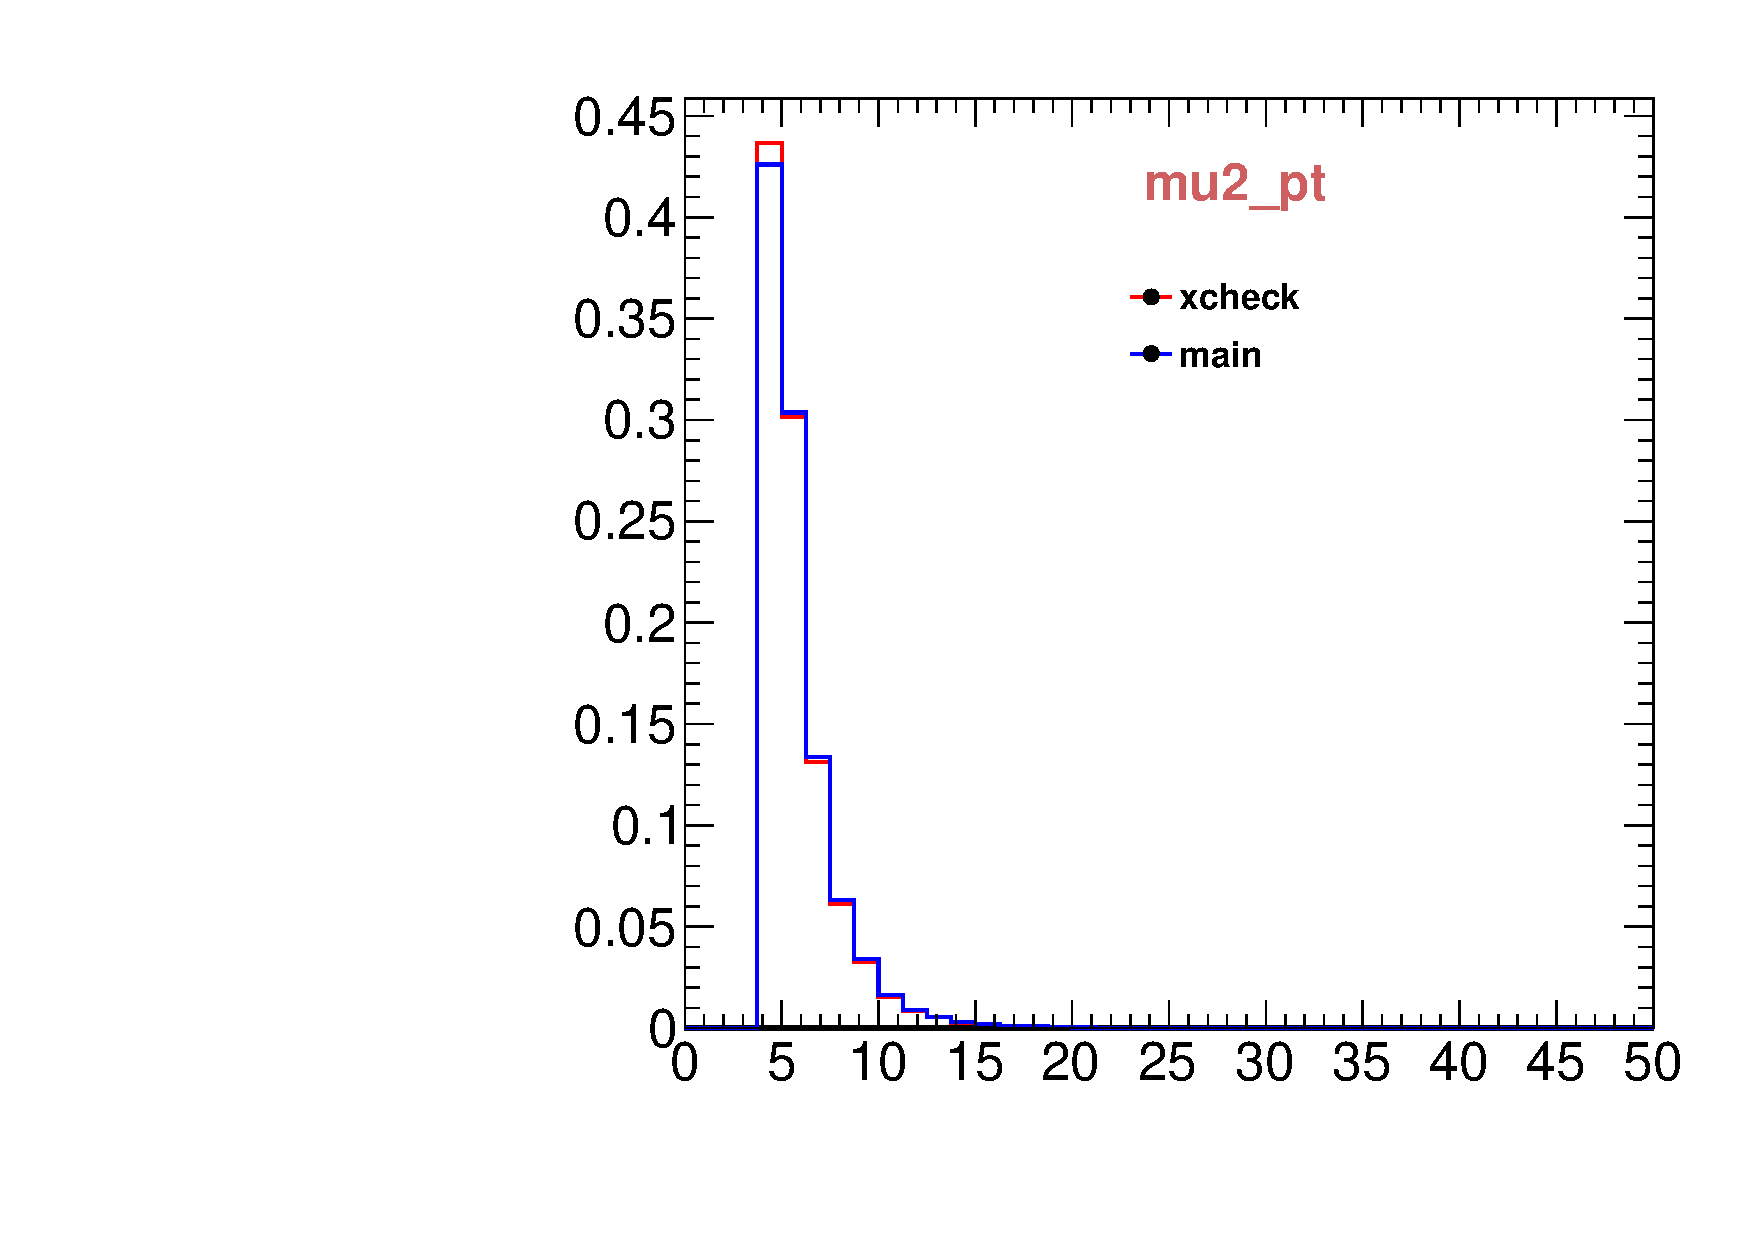
\includegraphics[width=\textwidth]{Figures/VariablesComparison/MC_endcaps_figs/m2pt}
                \label{fig:MC_endcaps_m2pt}
        \end{subfigure}
        \begin{subfigure}[b]{0.2\textwidth}
                \centering
                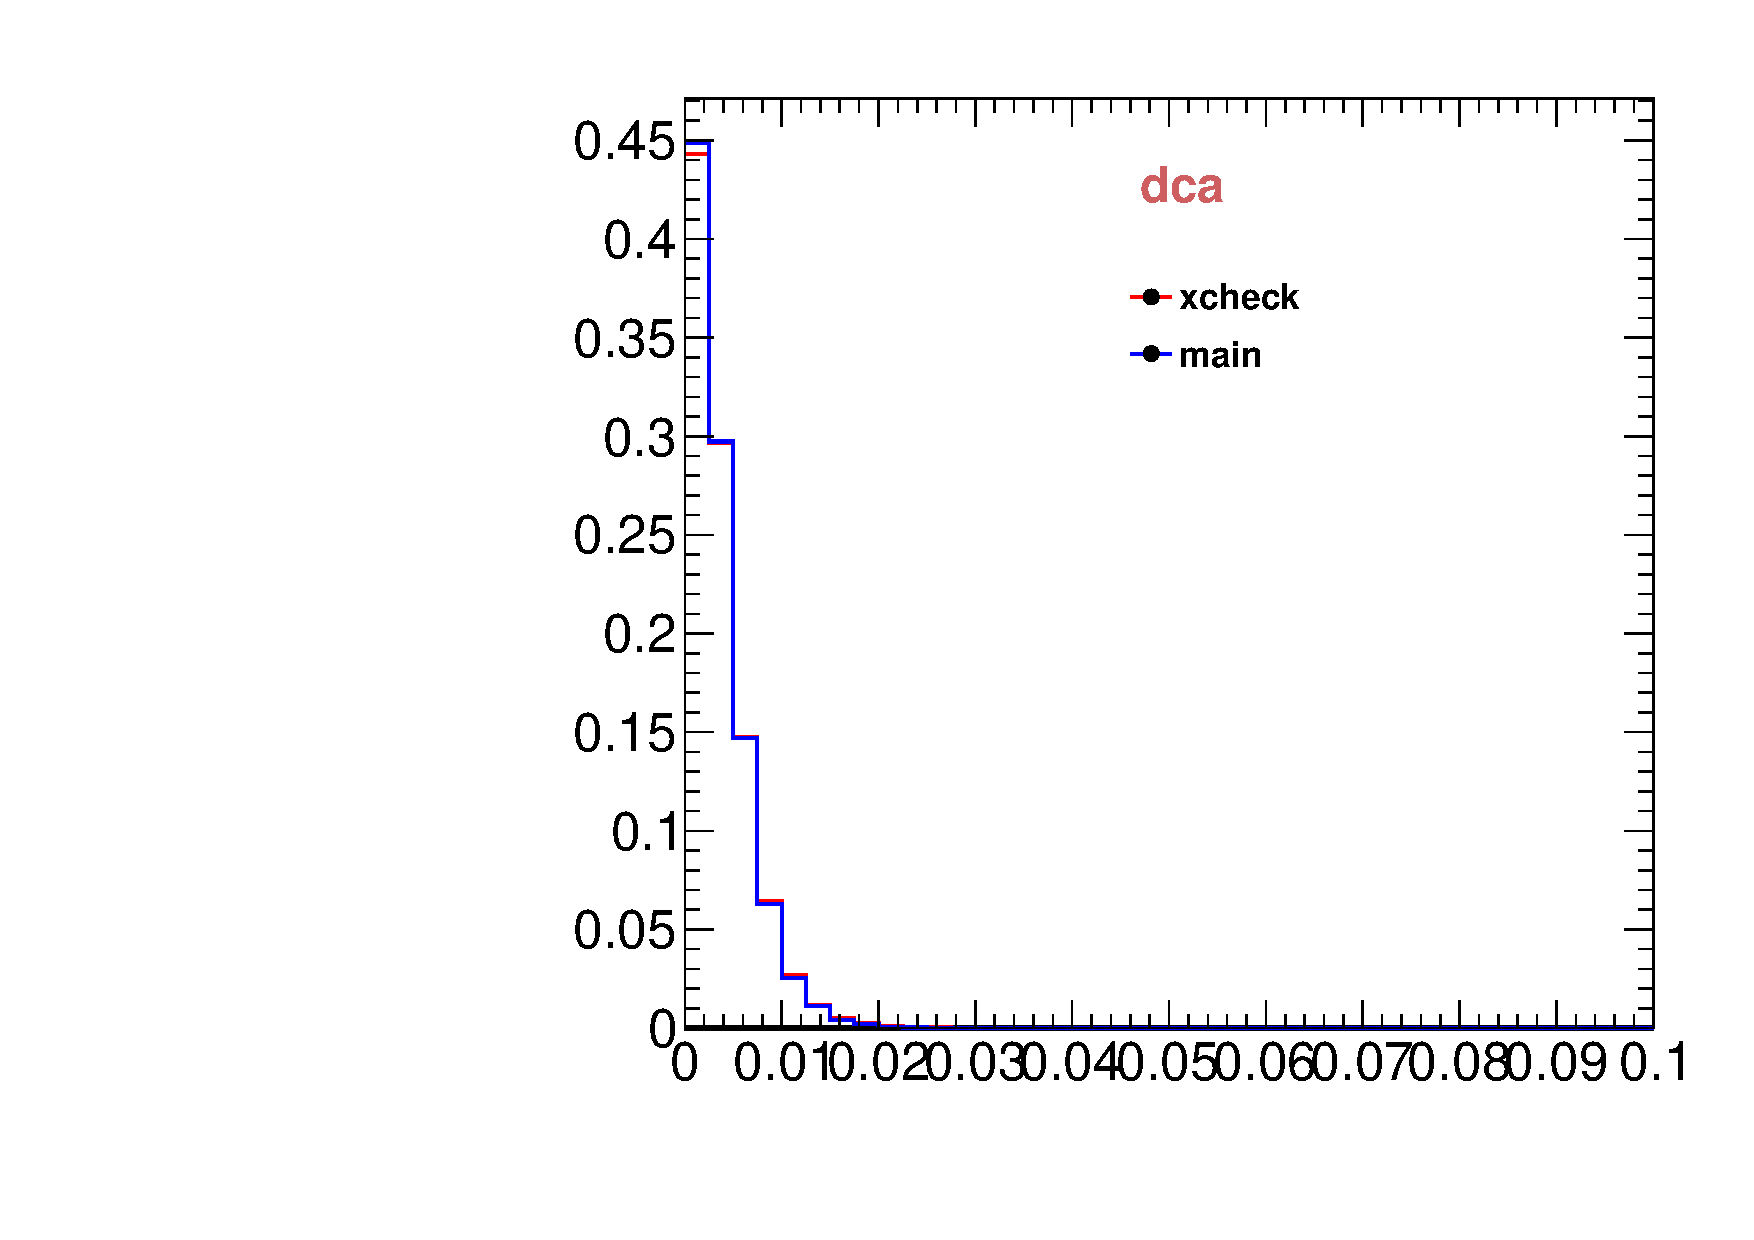
\includegraphics[width=\textwidth]{Figures/VariablesComparison/MC_endcaps_figs/maxdoca}
                \label{fig:MC_endcaps_maxdoca}
        \end{subfigure}
        \begin{subfigure}[b]{0.2\textwidth}
                \centering
                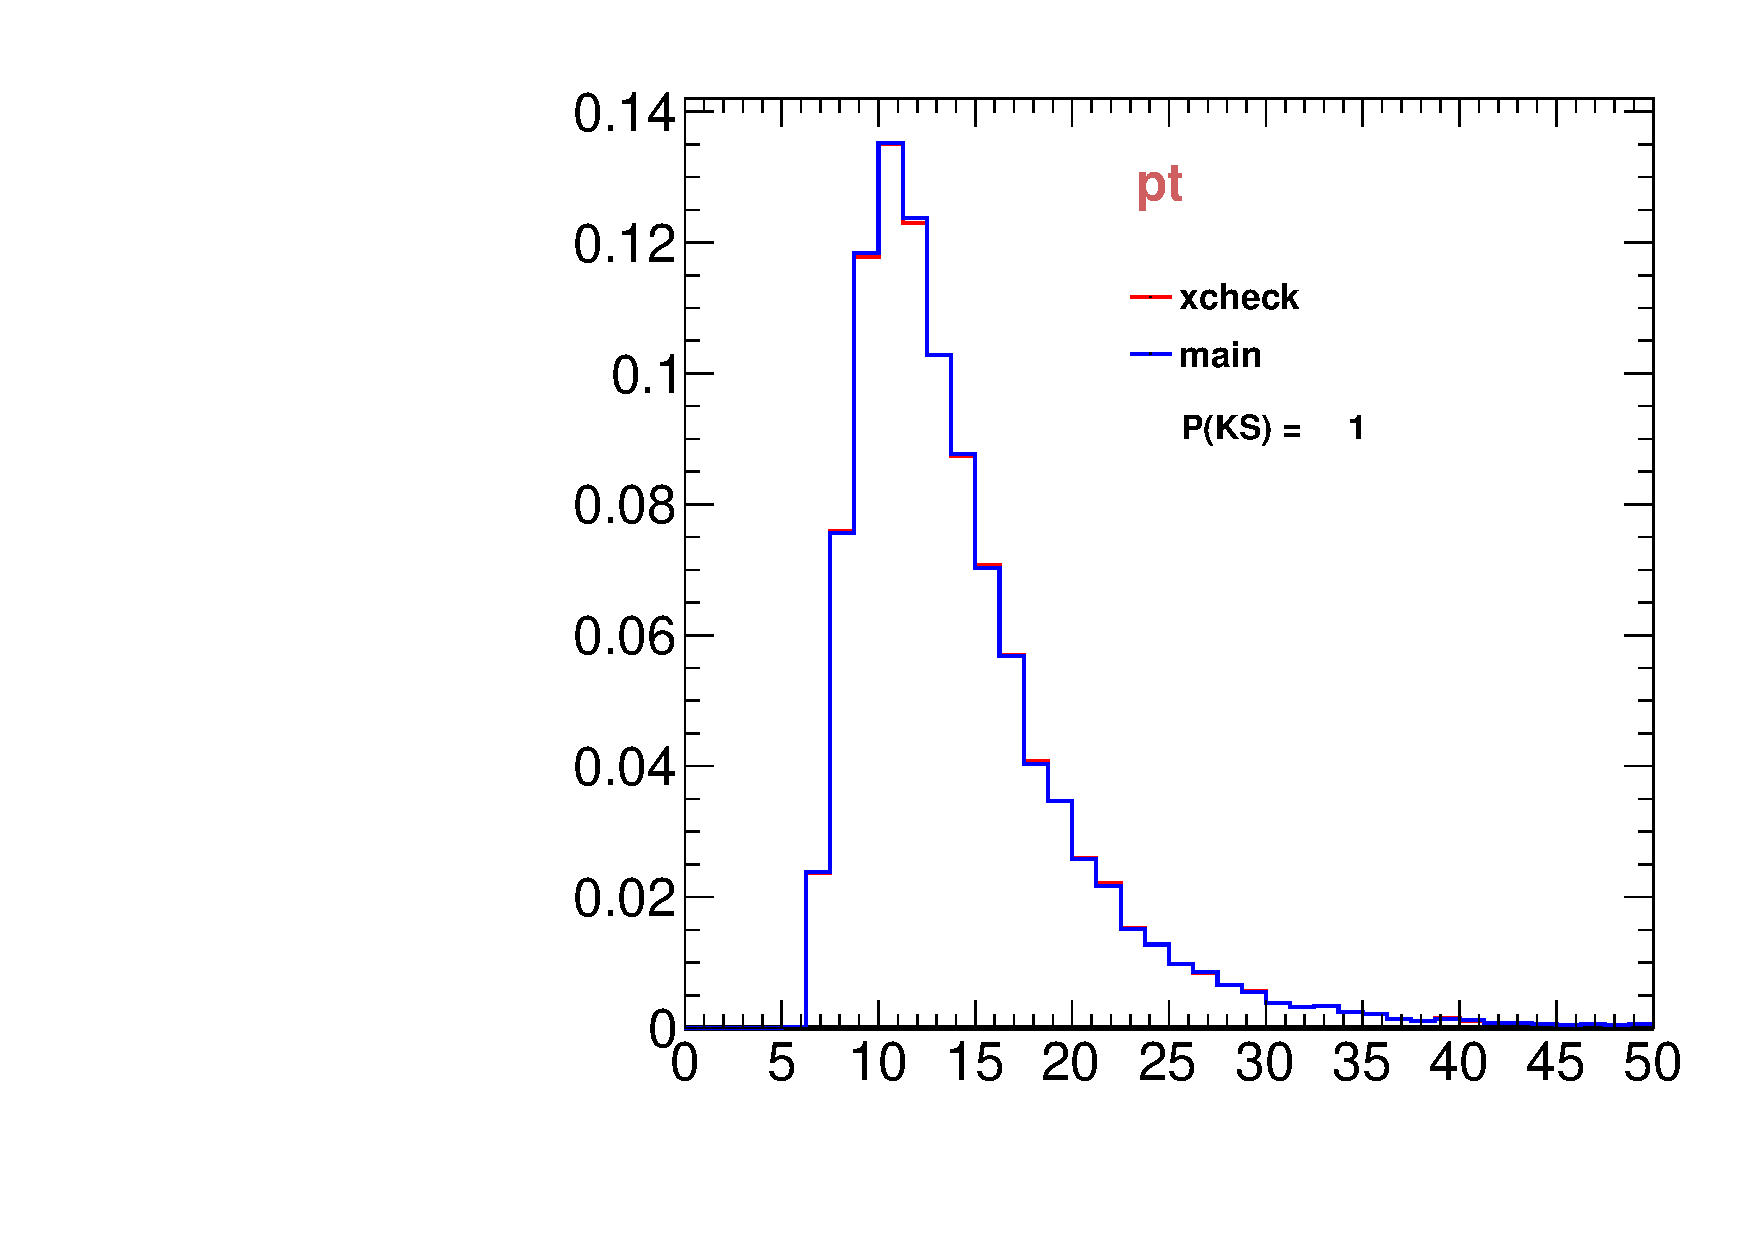
\includegraphics[width=\textwidth]{Figures/VariablesComparison/MC_endcaps_figs/pt}
                \label{fig:MC_endcaps_pt}
        \end{subfigure}
        \begin{subfigure}[b]{0.2\textwidth}
                \centering
                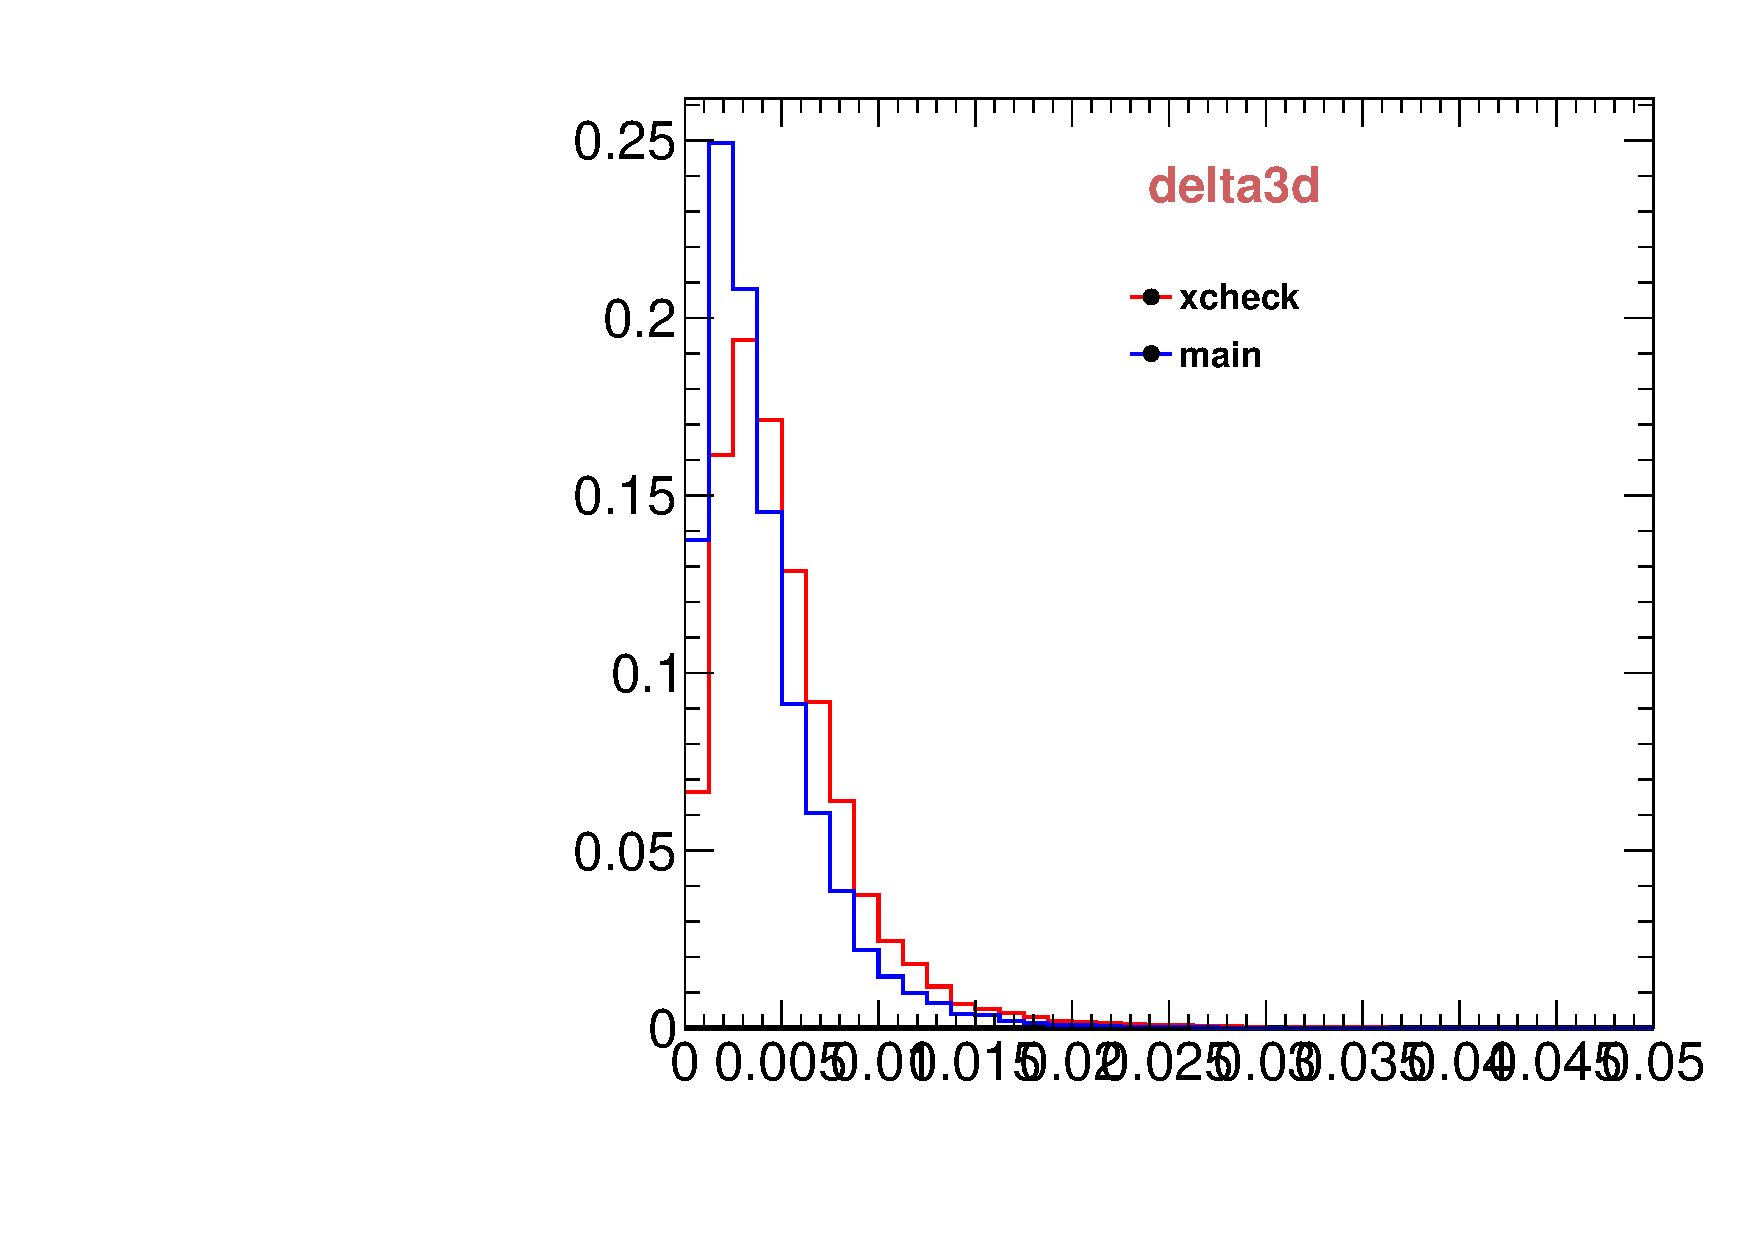
\includegraphics[width=\textwidth]{Figures/VariablesComparison/MC_endcaps_figs/pvip}
                \label{fig:MC_endcaps_pvip}
        \end{subfigure}
        \begin{subfigure}[b]{0.2\textwidth}
                \centering
                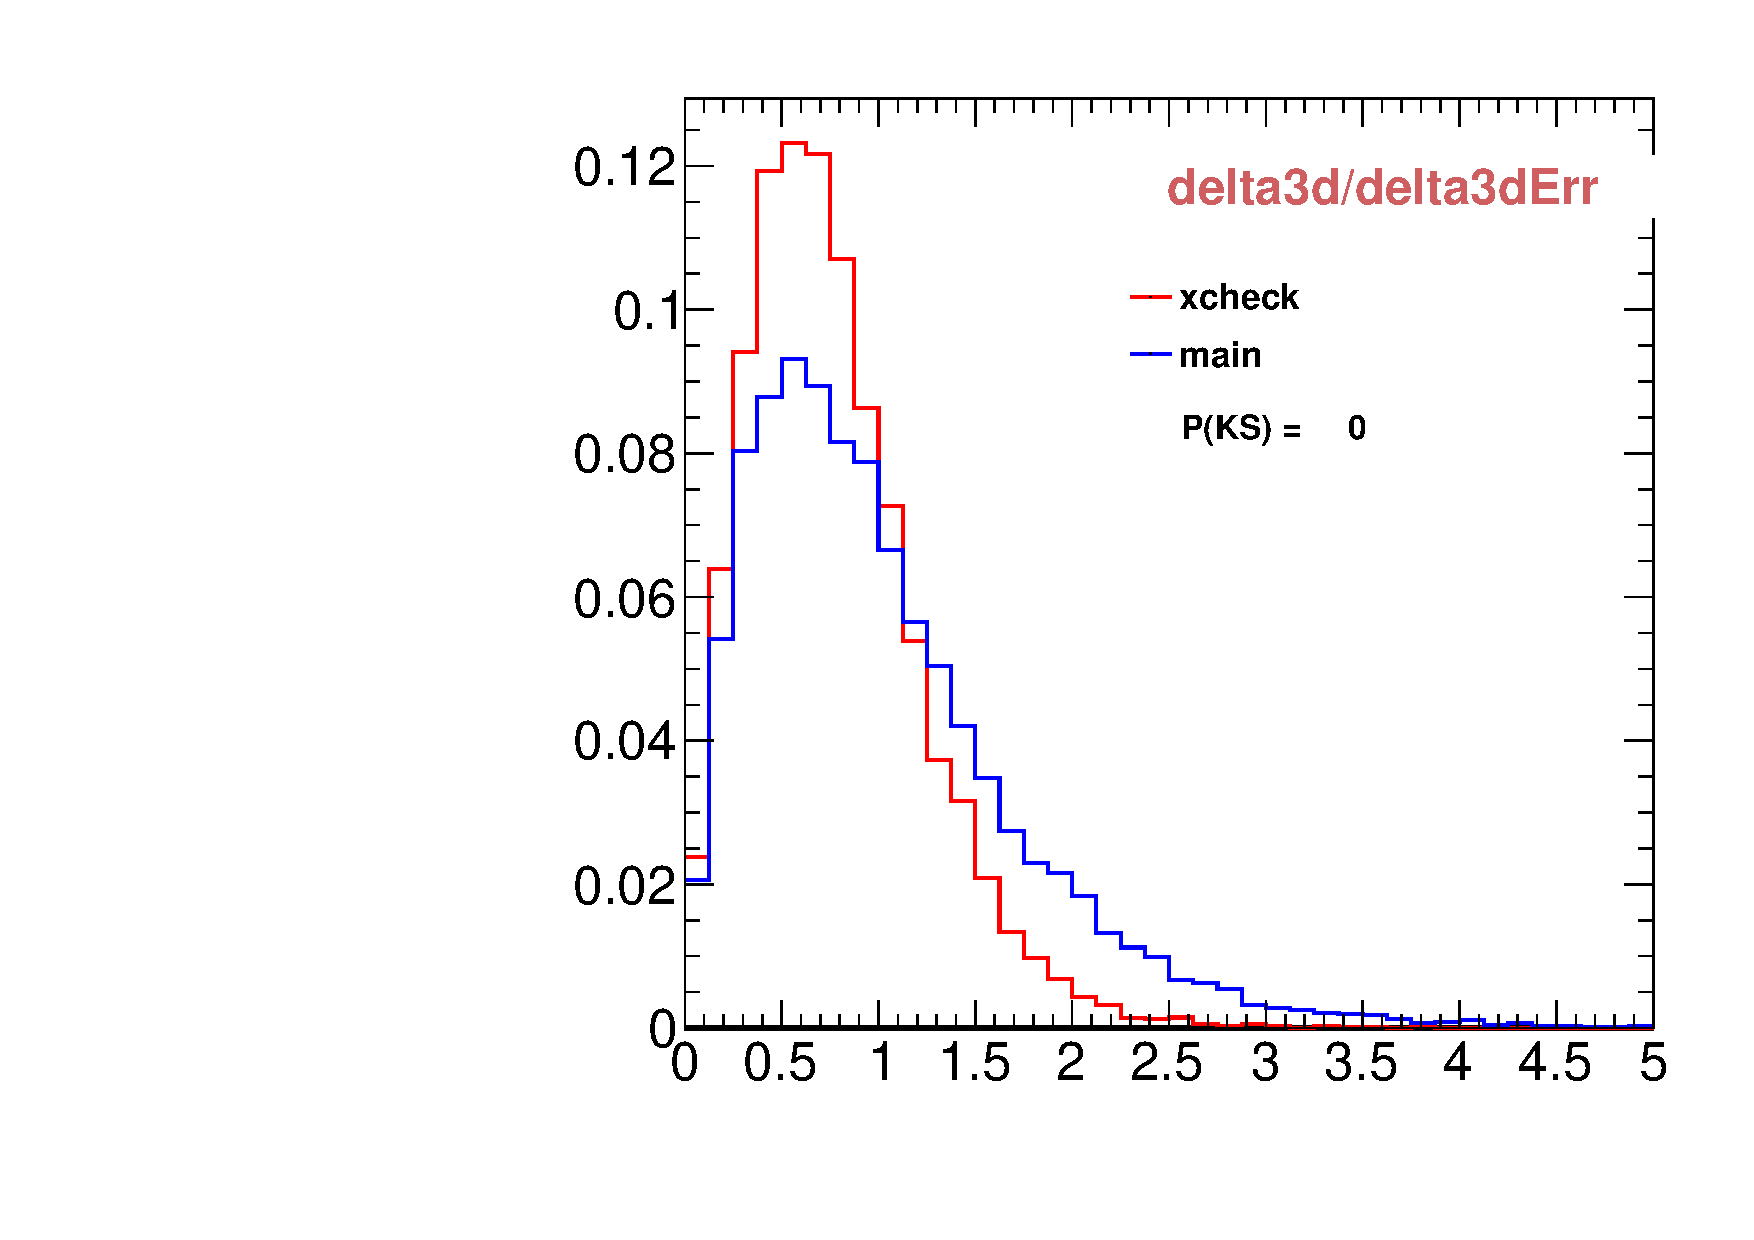
\includegraphics[width=\textwidth]{Figures/VariablesComparison/MC_endcaps_figs/pvips}
                \label{fig:MC_endcaps_pvips}
        \end{subfigure}
        \begin{subfigure}[b]{0.2\textwidth}
                \centering
                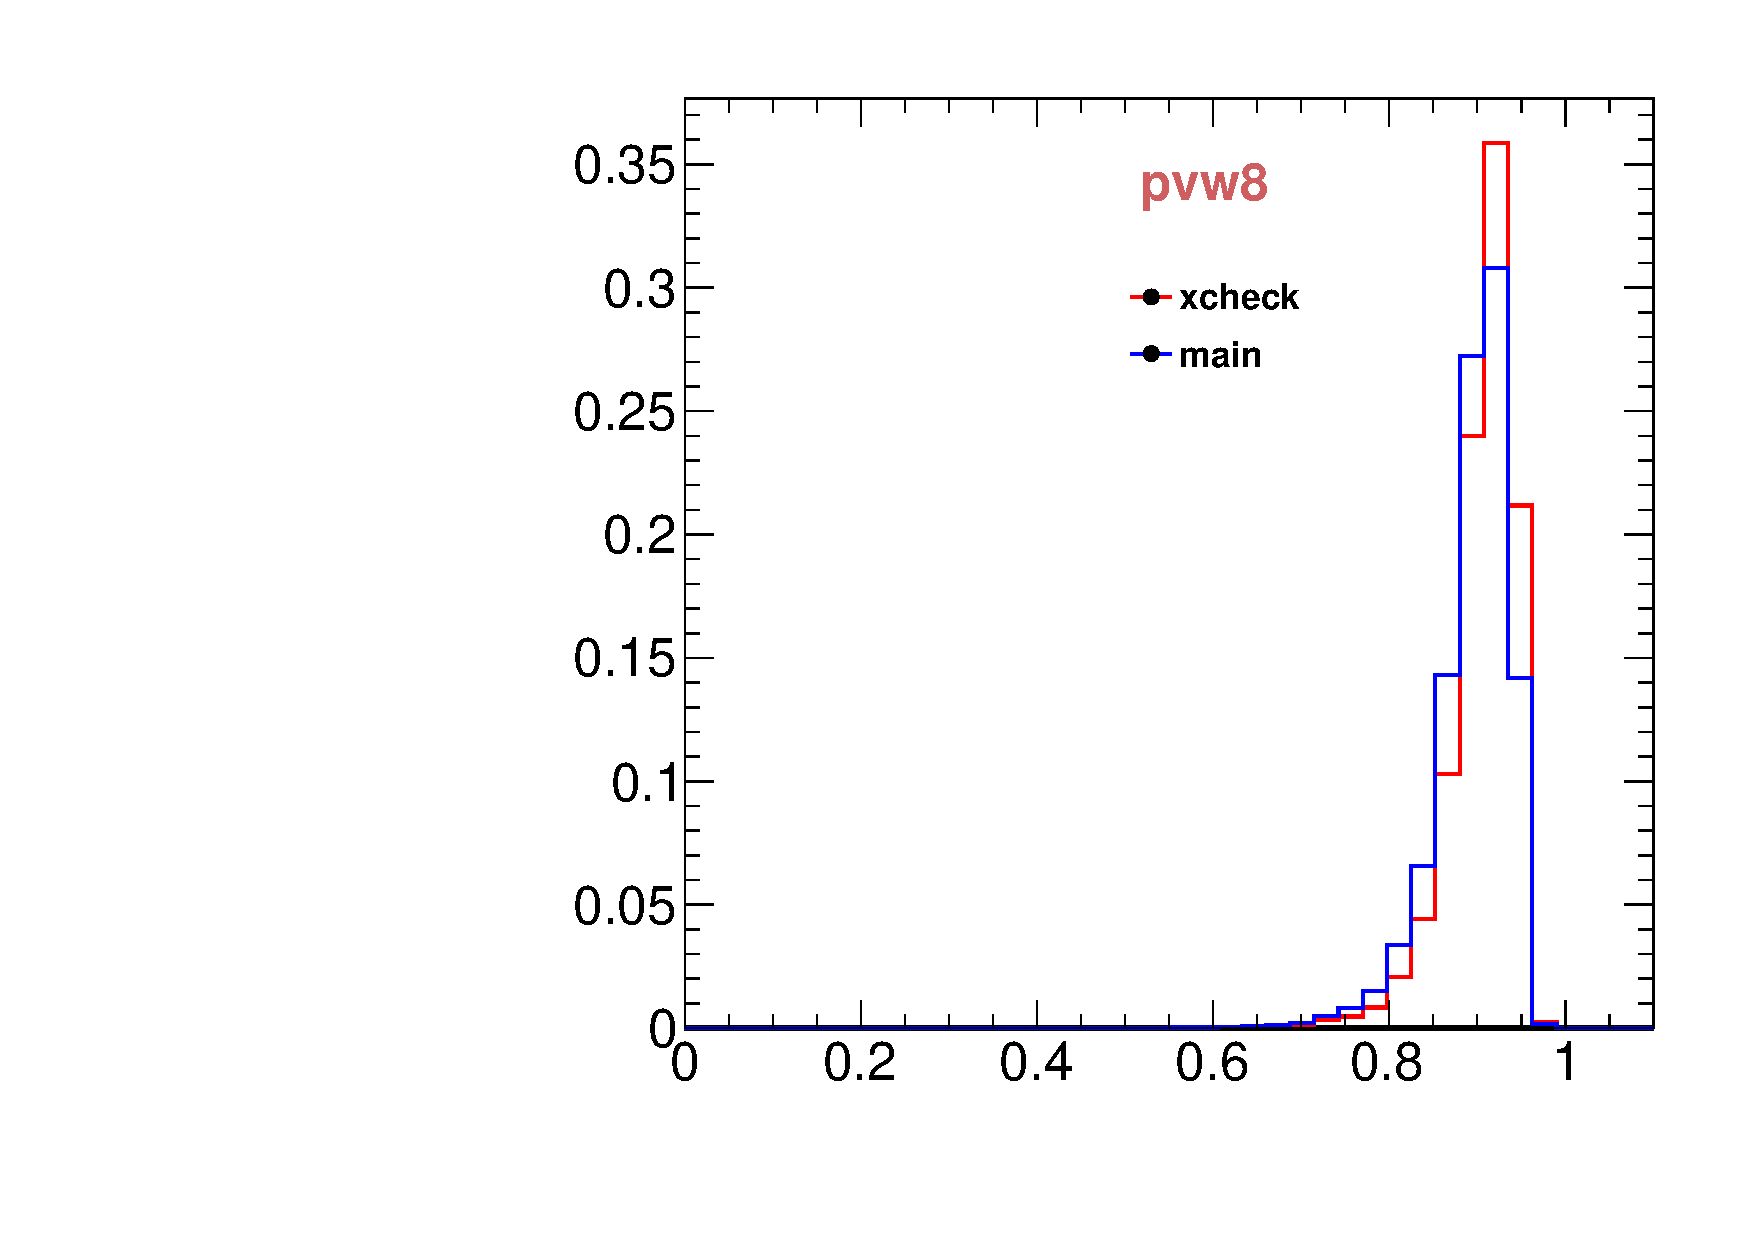
\includegraphics[width=\textwidth]{Figures/VariablesComparison/MC_endcaps_figs/pvw8}
                \label{fig:MC_endcaps_pvw8}
        \end{subfigure}
        \caption{Variable comparisons between the main analysis and the cross-check analysis. Part I: MC endcaps.}
        \label{fig:MC_endcaps_figs}
\end{sidewaysfigure}


\begin{sidewaysfigure}
        \centering
        \begin{subfigure}[b]{0.2\textwidth}
                \centering
                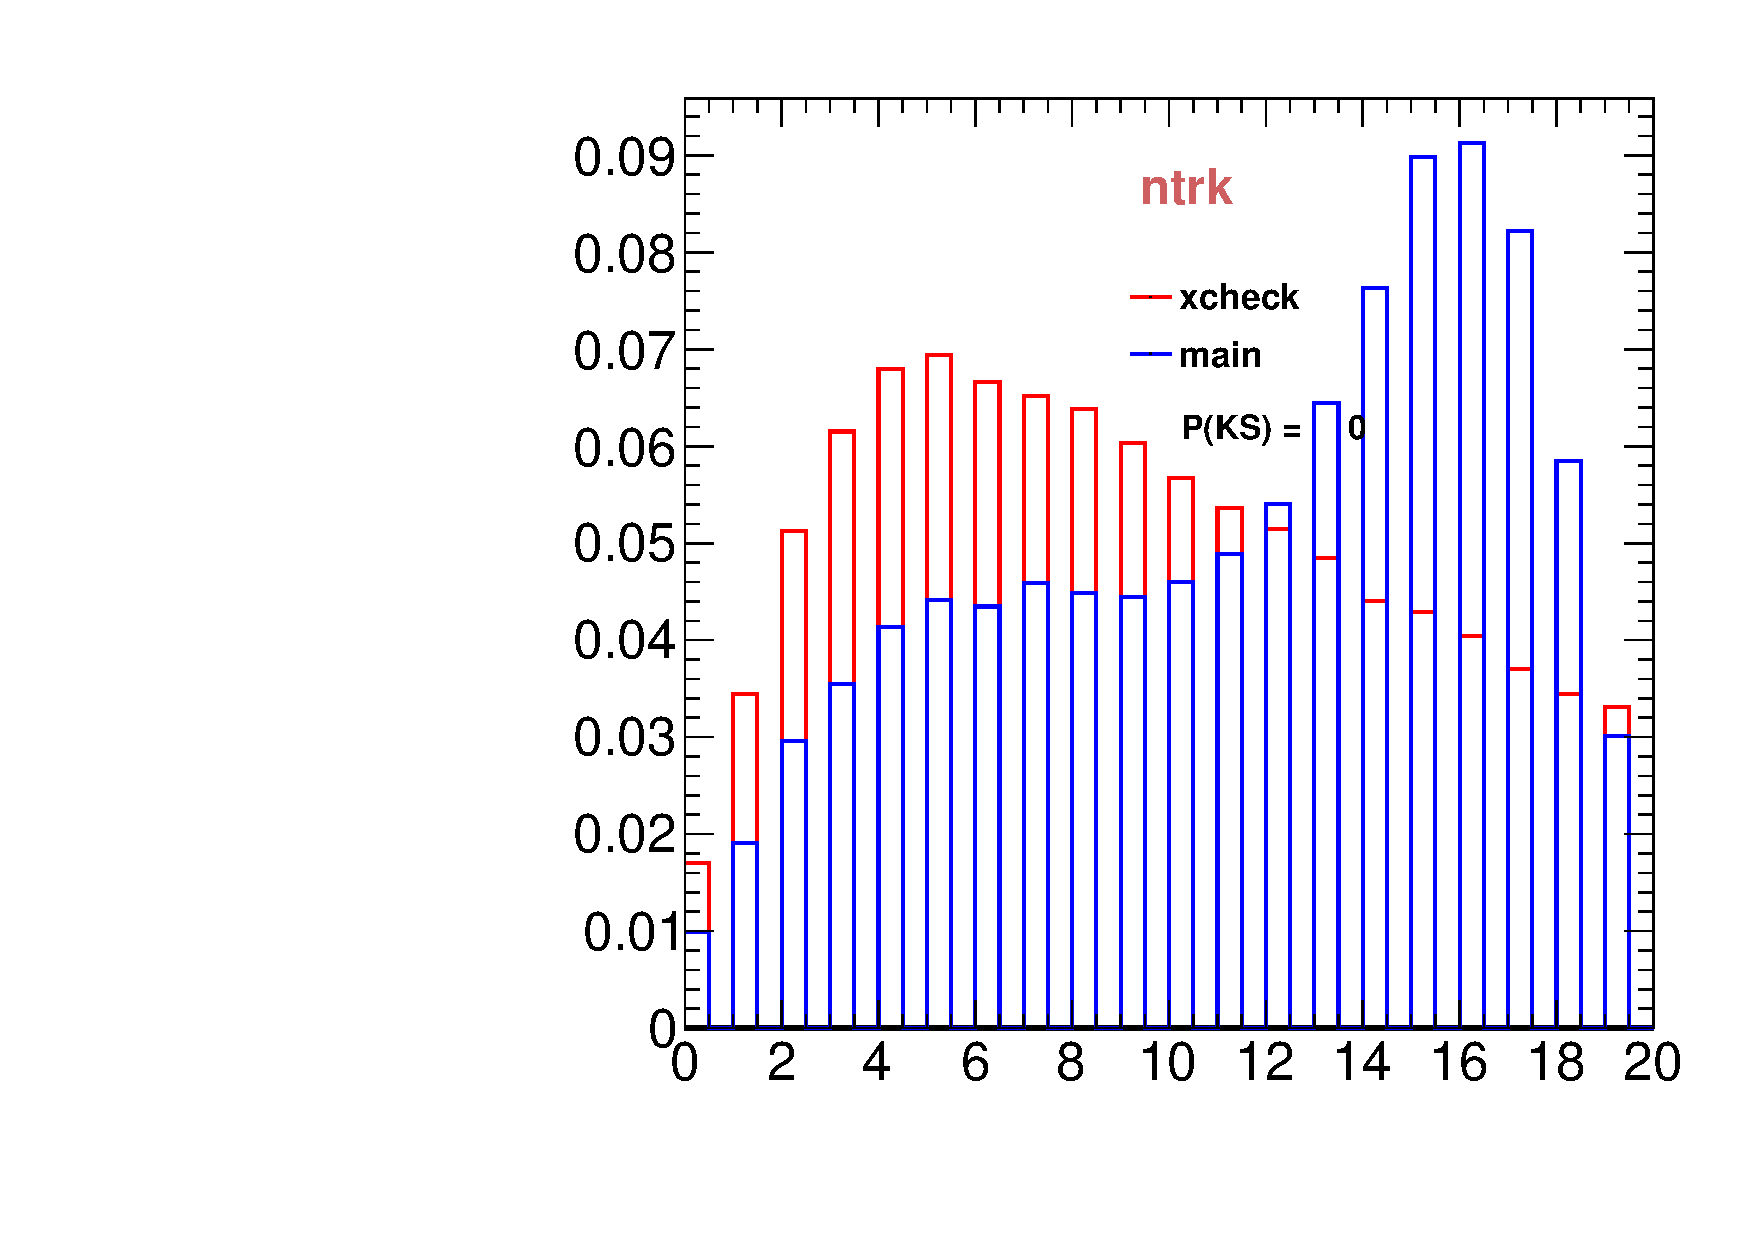
\includegraphics[width=\textwidth]{Figures/VariablesComparison/Data_barrel_figs/closetrk}
                \label{fig:Data_barrel_closetrk}
        \end{subfigure}
        \begin{subfigure}[b]{0.2\textwidth}
                \centering
                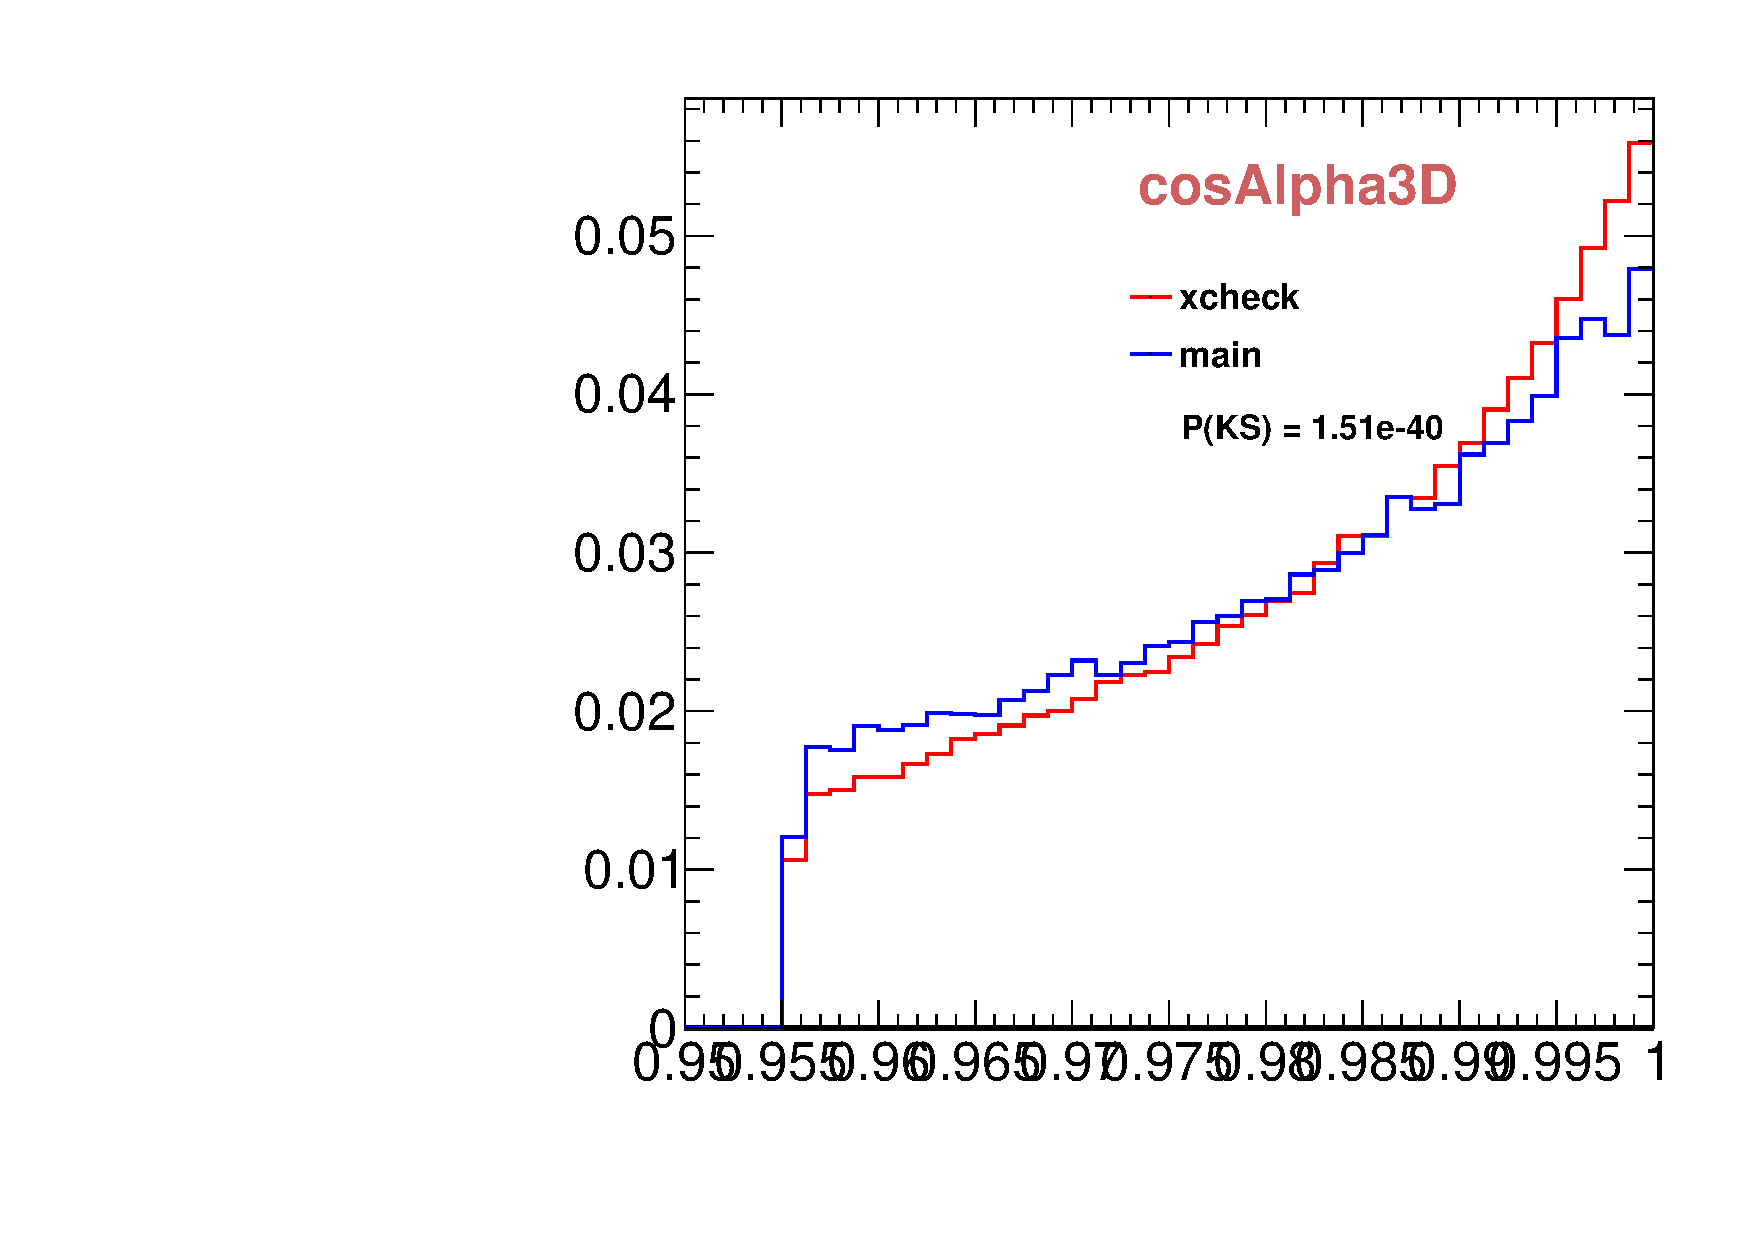
\includegraphics[width=\textwidth]{Figures/VariablesComparison/Data_barrel_figs/cosa}
                \label{fig:Data_barrel_cosa}
        \end{subfigure}
        \begin{subfigure}[b]{0.2\textwidth}
                \centering
                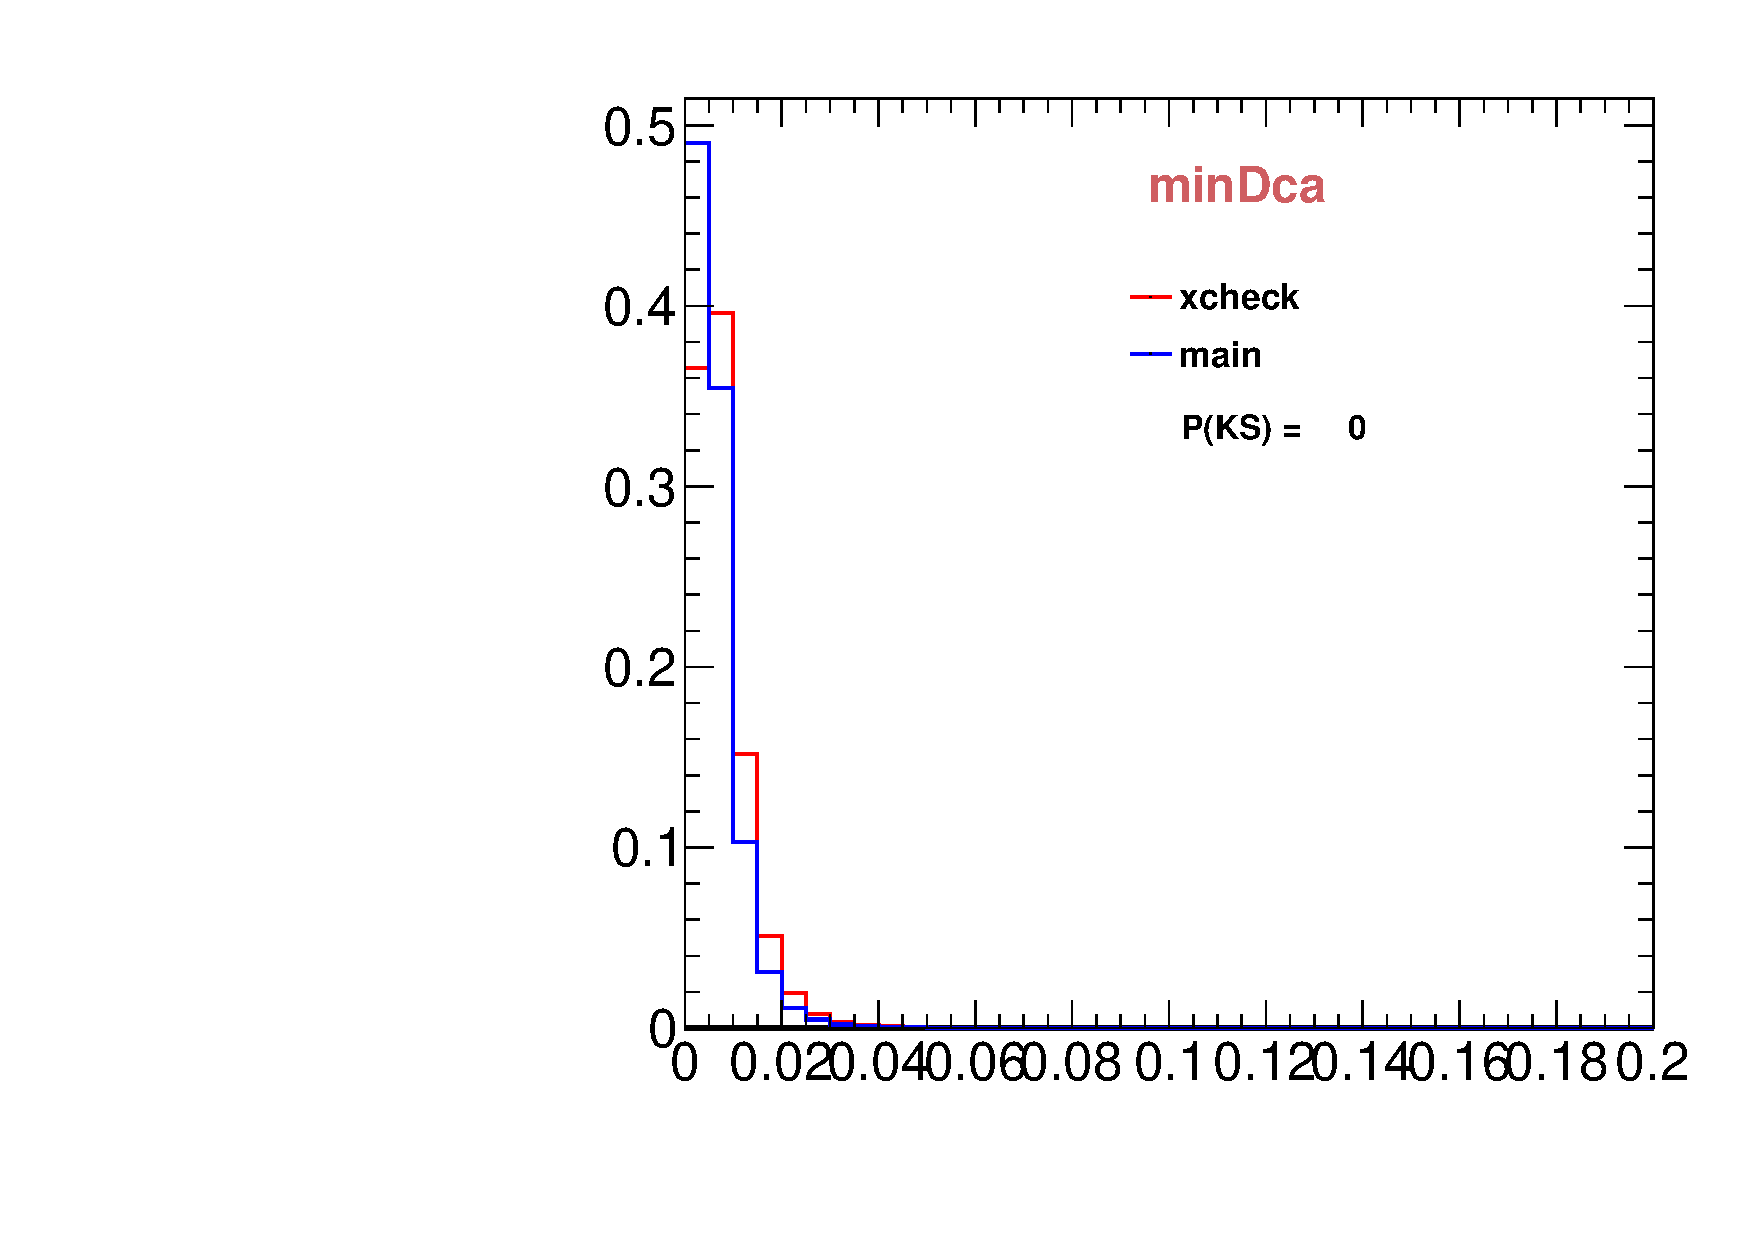
\includegraphics[width=\textwidth]{Figures/VariablesComparison/Data_barrel_figs/docatrk}
                \label{fig:Data_barrel_docatrk}
        \end{subfigure}
        \begin{subfigure}[b]{0.2\textwidth}
                \centering
                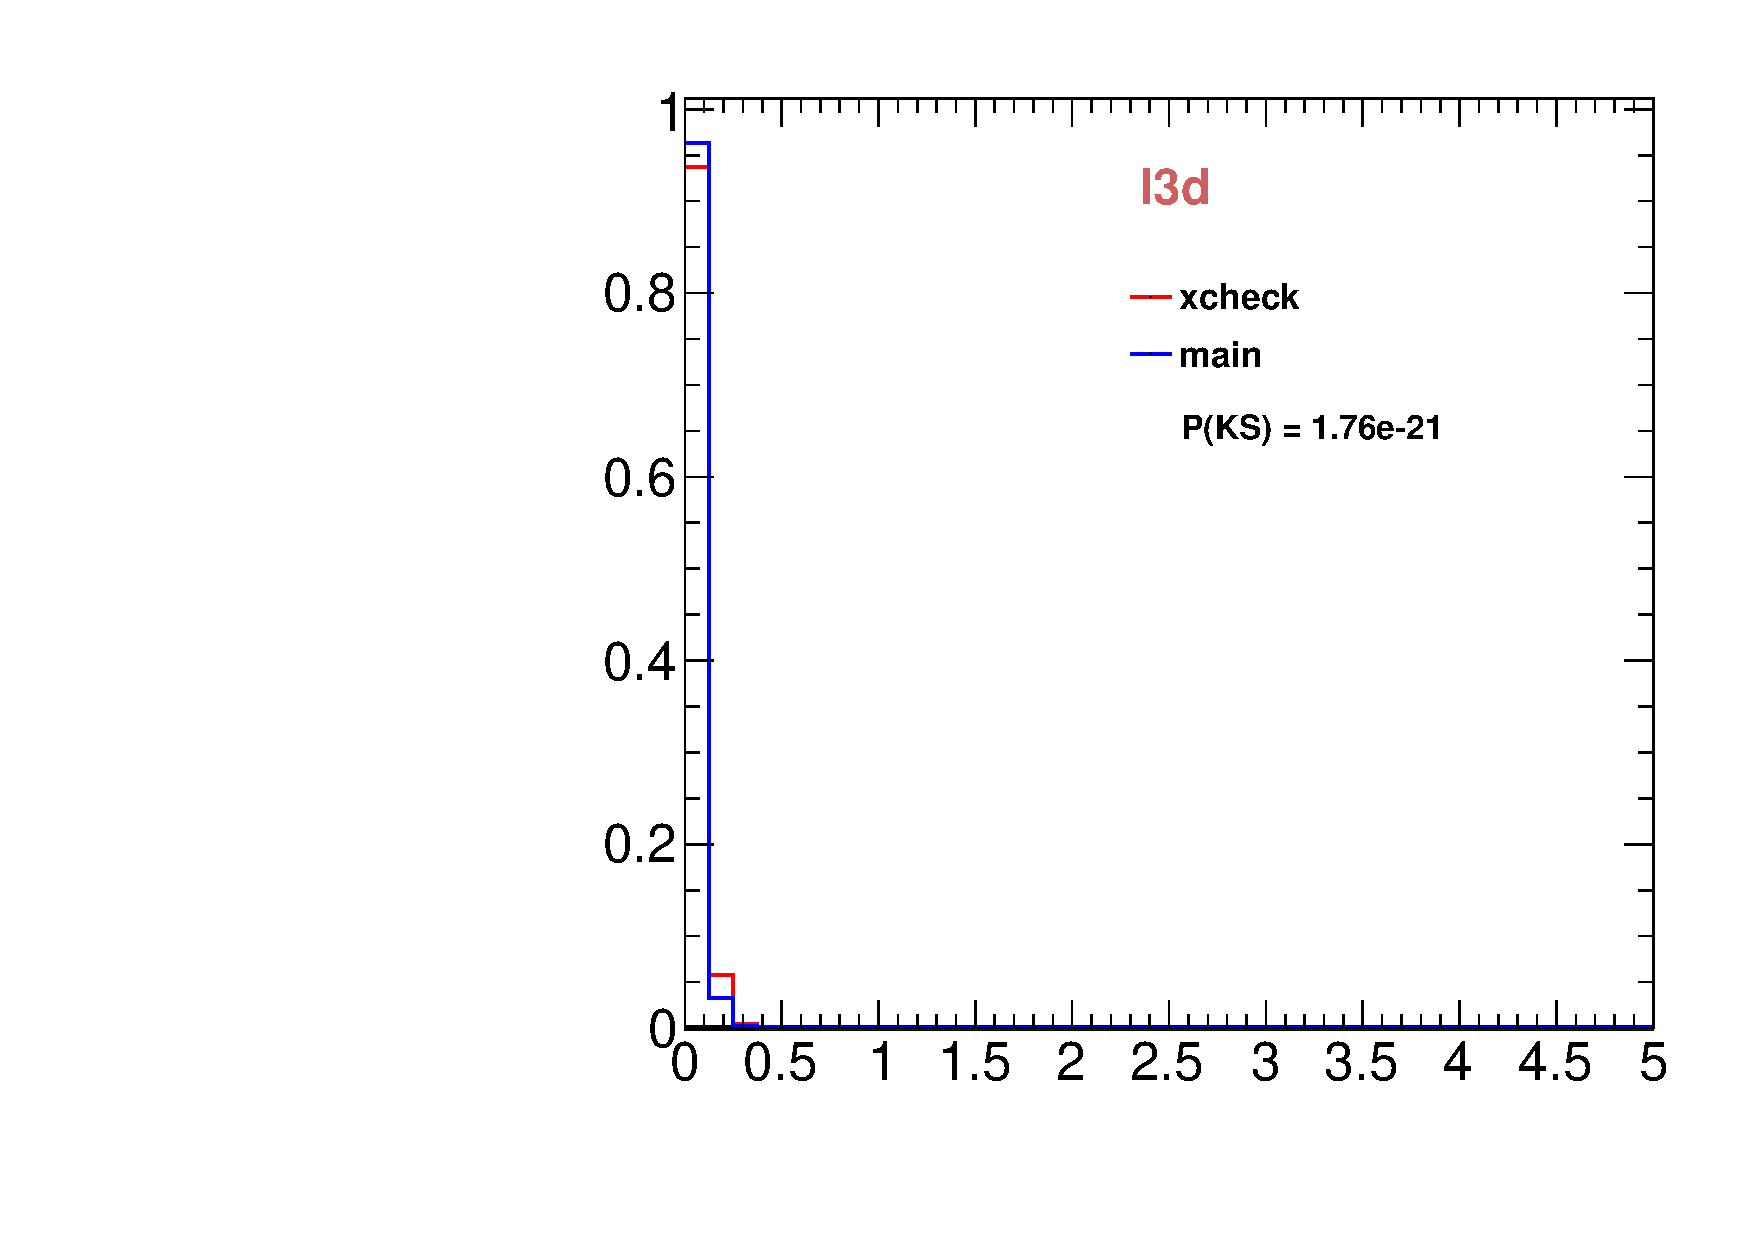
\includegraphics[width=\textwidth]{Figures/VariablesComparison/Data_barrel_figs/fl3d}
                \label{fig:Data_barrel_fl3d}
        \end{subfigure}
        \begin{subfigure}[b]{0.2\textwidth}
                \centering
                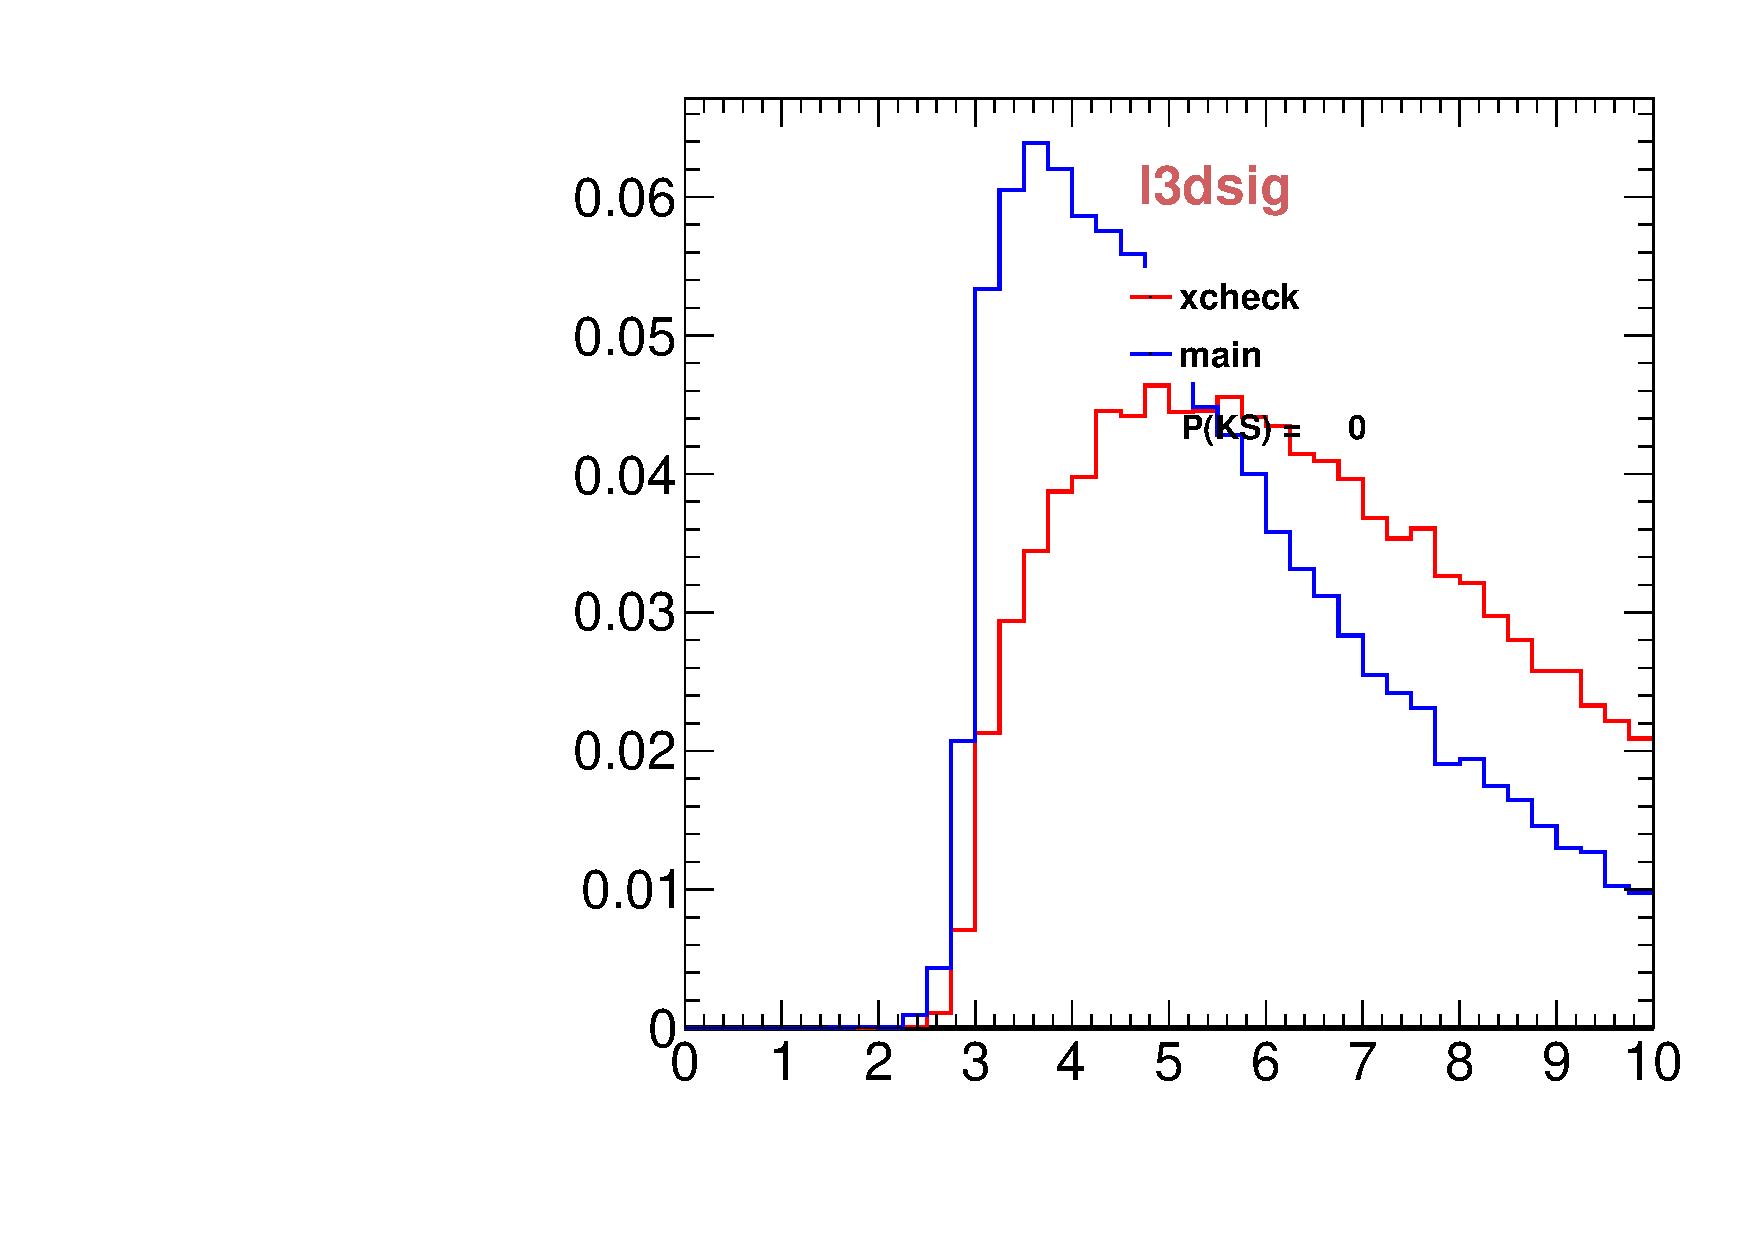
\includegraphics[width=\textwidth]{Figures/VariablesComparison/Data_barrel_figs/fls3d}
                \label{fig:Data_barrel_fls3d}
        \end{subfigure}
        \begin{subfigure}[b]{0.2\textwidth}
                \centering
                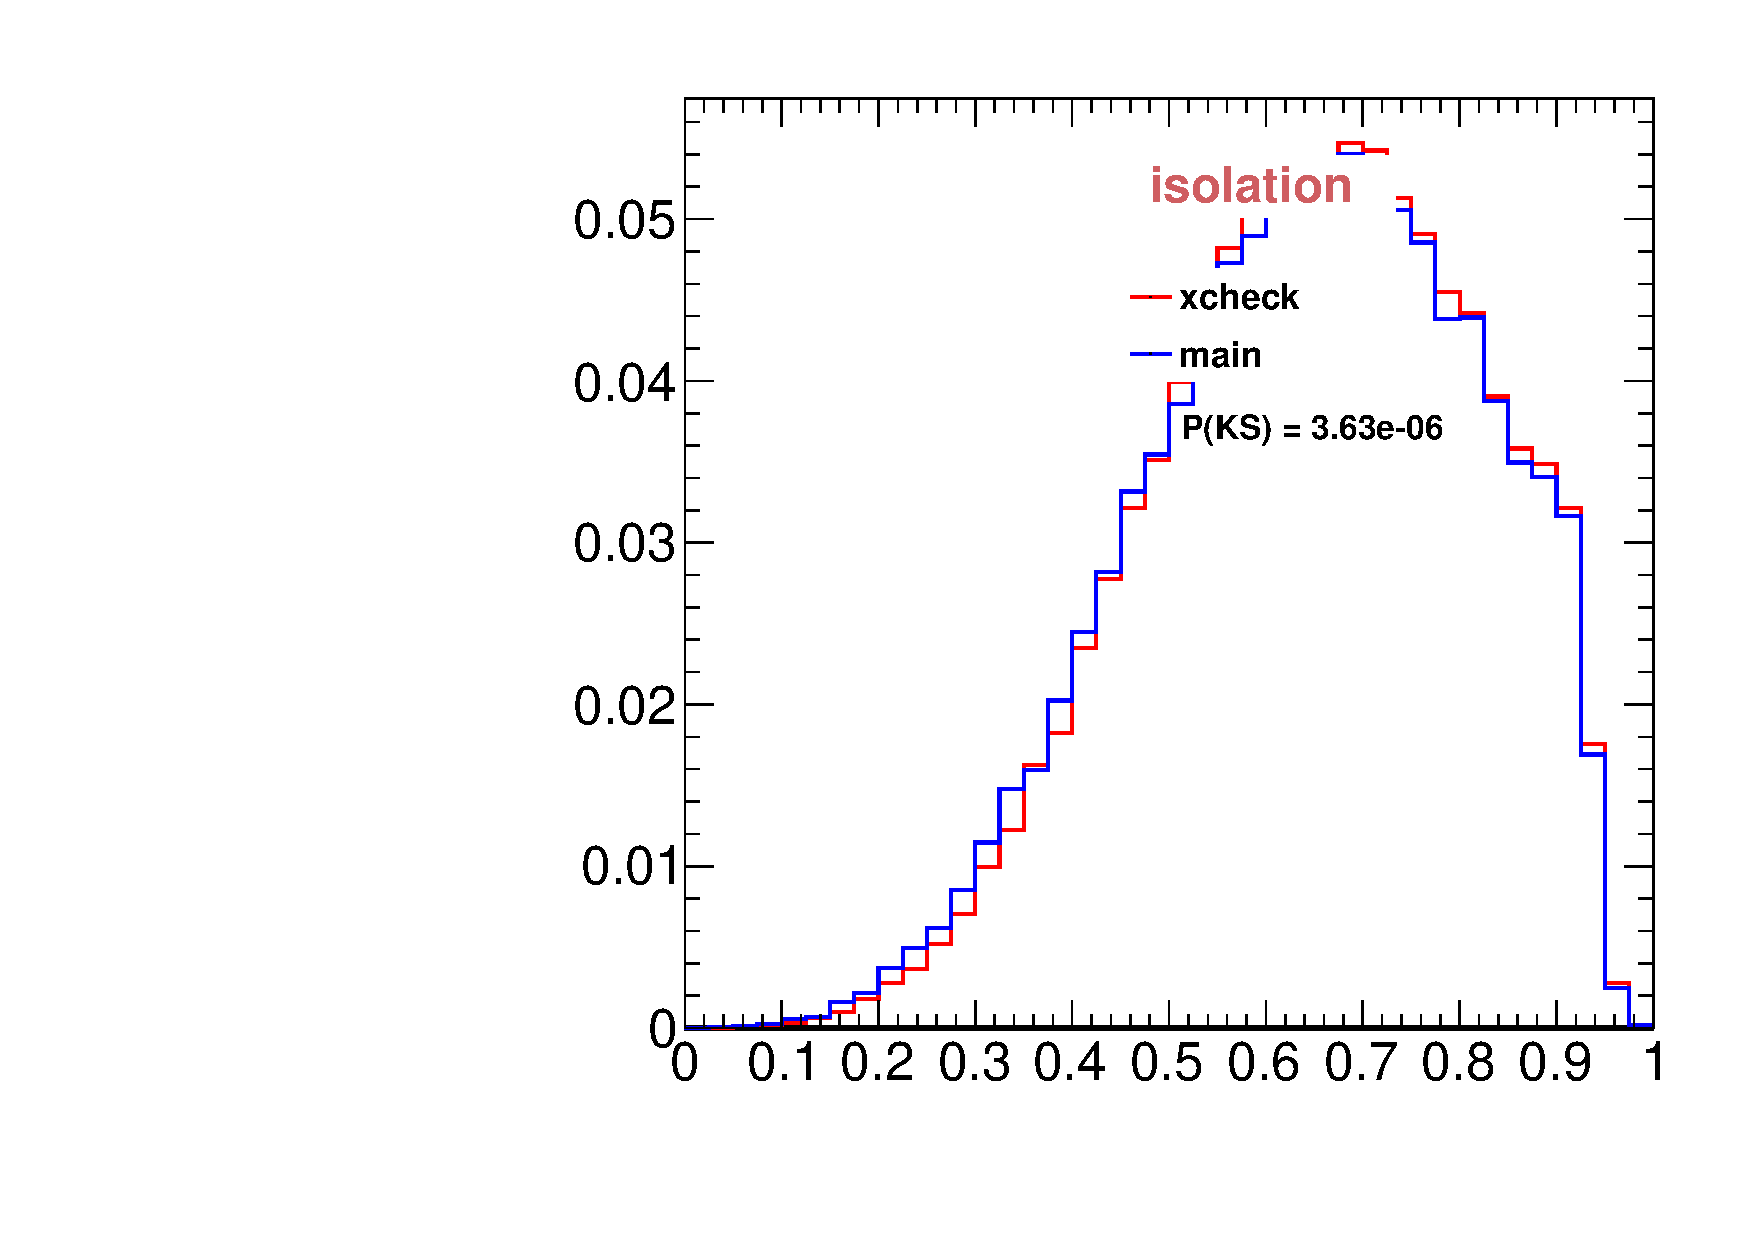
\includegraphics[width=\textwidth]{Figures/VariablesComparison/Data_barrel_figs/iso}
                \label{fig:Data_barrel_iso}
        \end{subfigure}
        \begin{subfigure}[b]{0.2\textwidth}
                \centering
                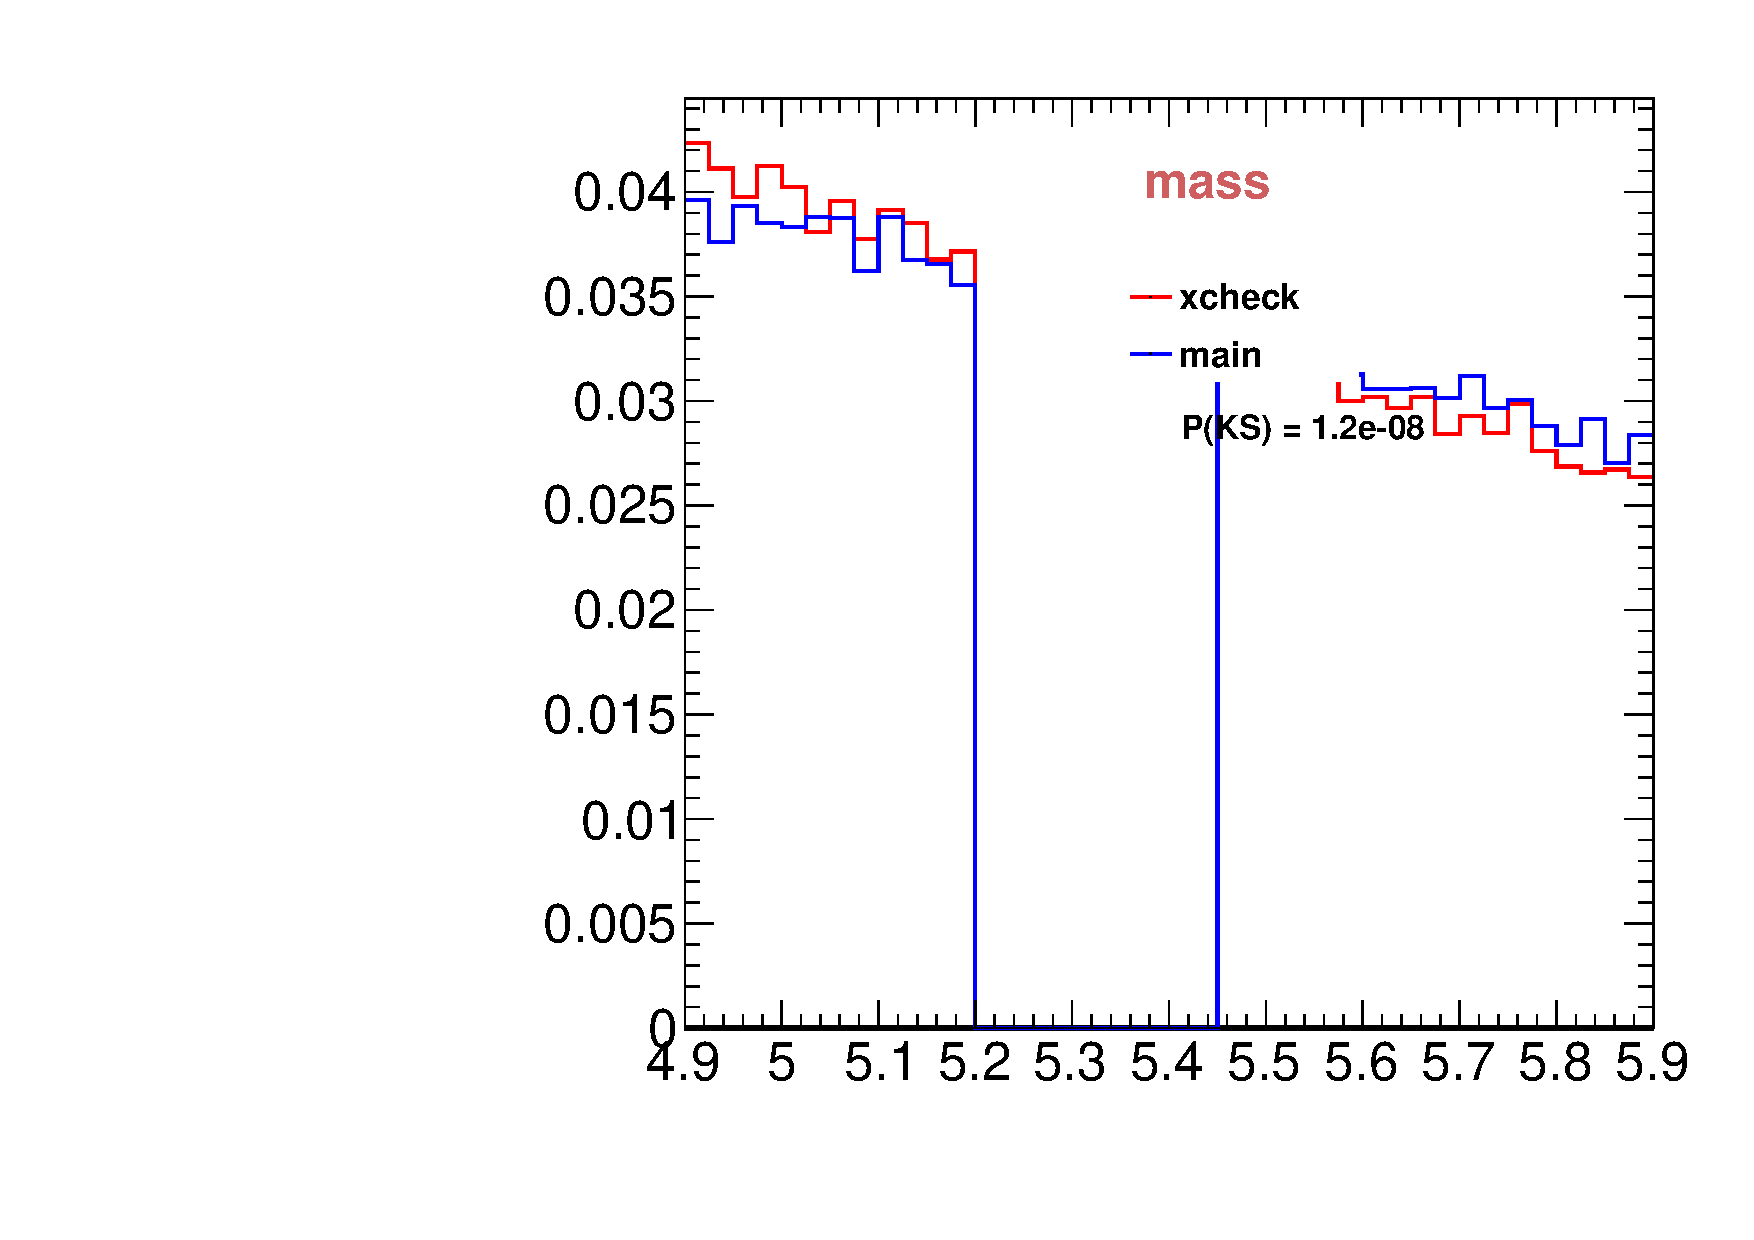
\includegraphics[width=\textwidth]{Figures/VariablesComparison/Data_barrel_figs/m}
                \label{fig:Data_barrel_m}
        \end{subfigure}
        \begin{subfigure}[b]{0.2\textwidth}
                \centering
                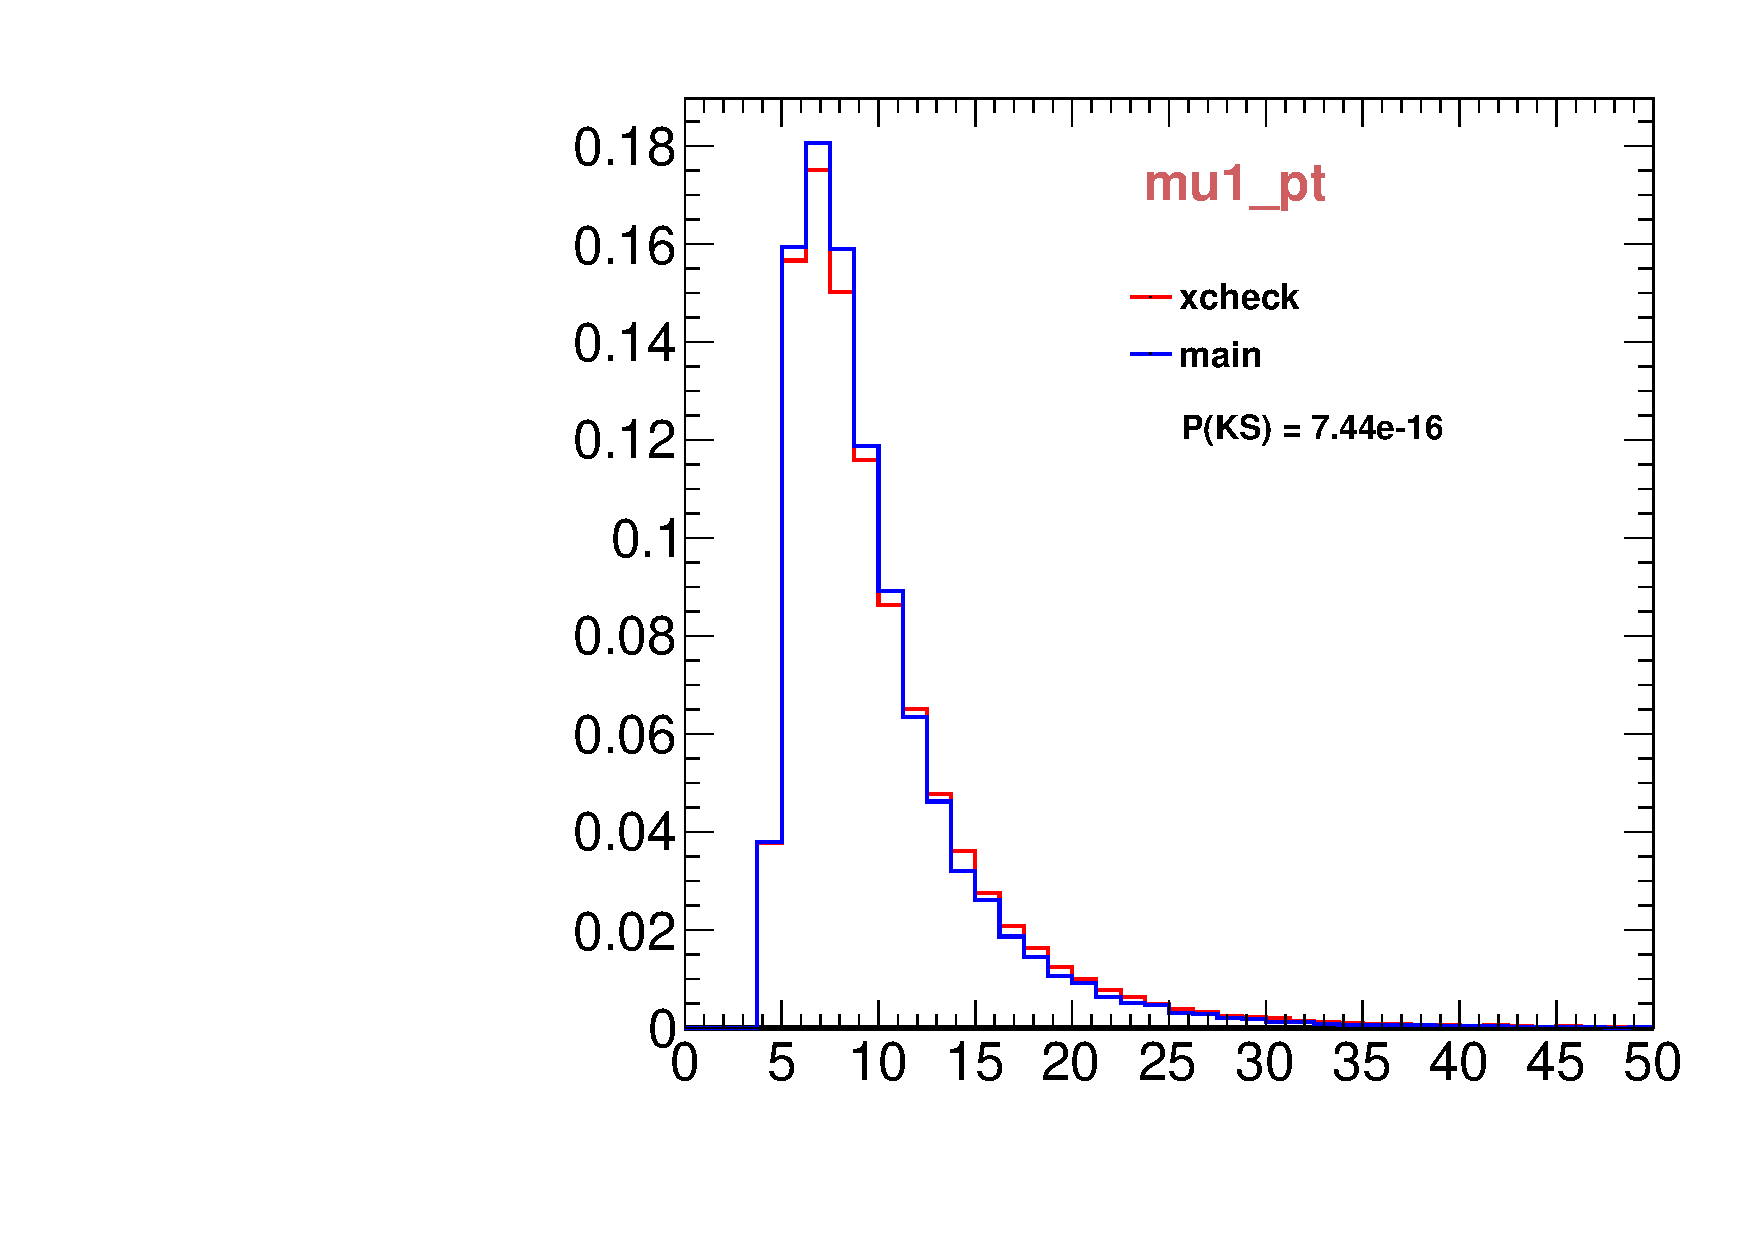
\includegraphics[width=\textwidth]{Figures/VariablesComparison/Data_barrel_figs/m1pt}
                \label{fig:Data_barrel_m1pt}
        \end{subfigure}
        \begin{subfigure}[b]{0.2\textwidth}
                \centering
                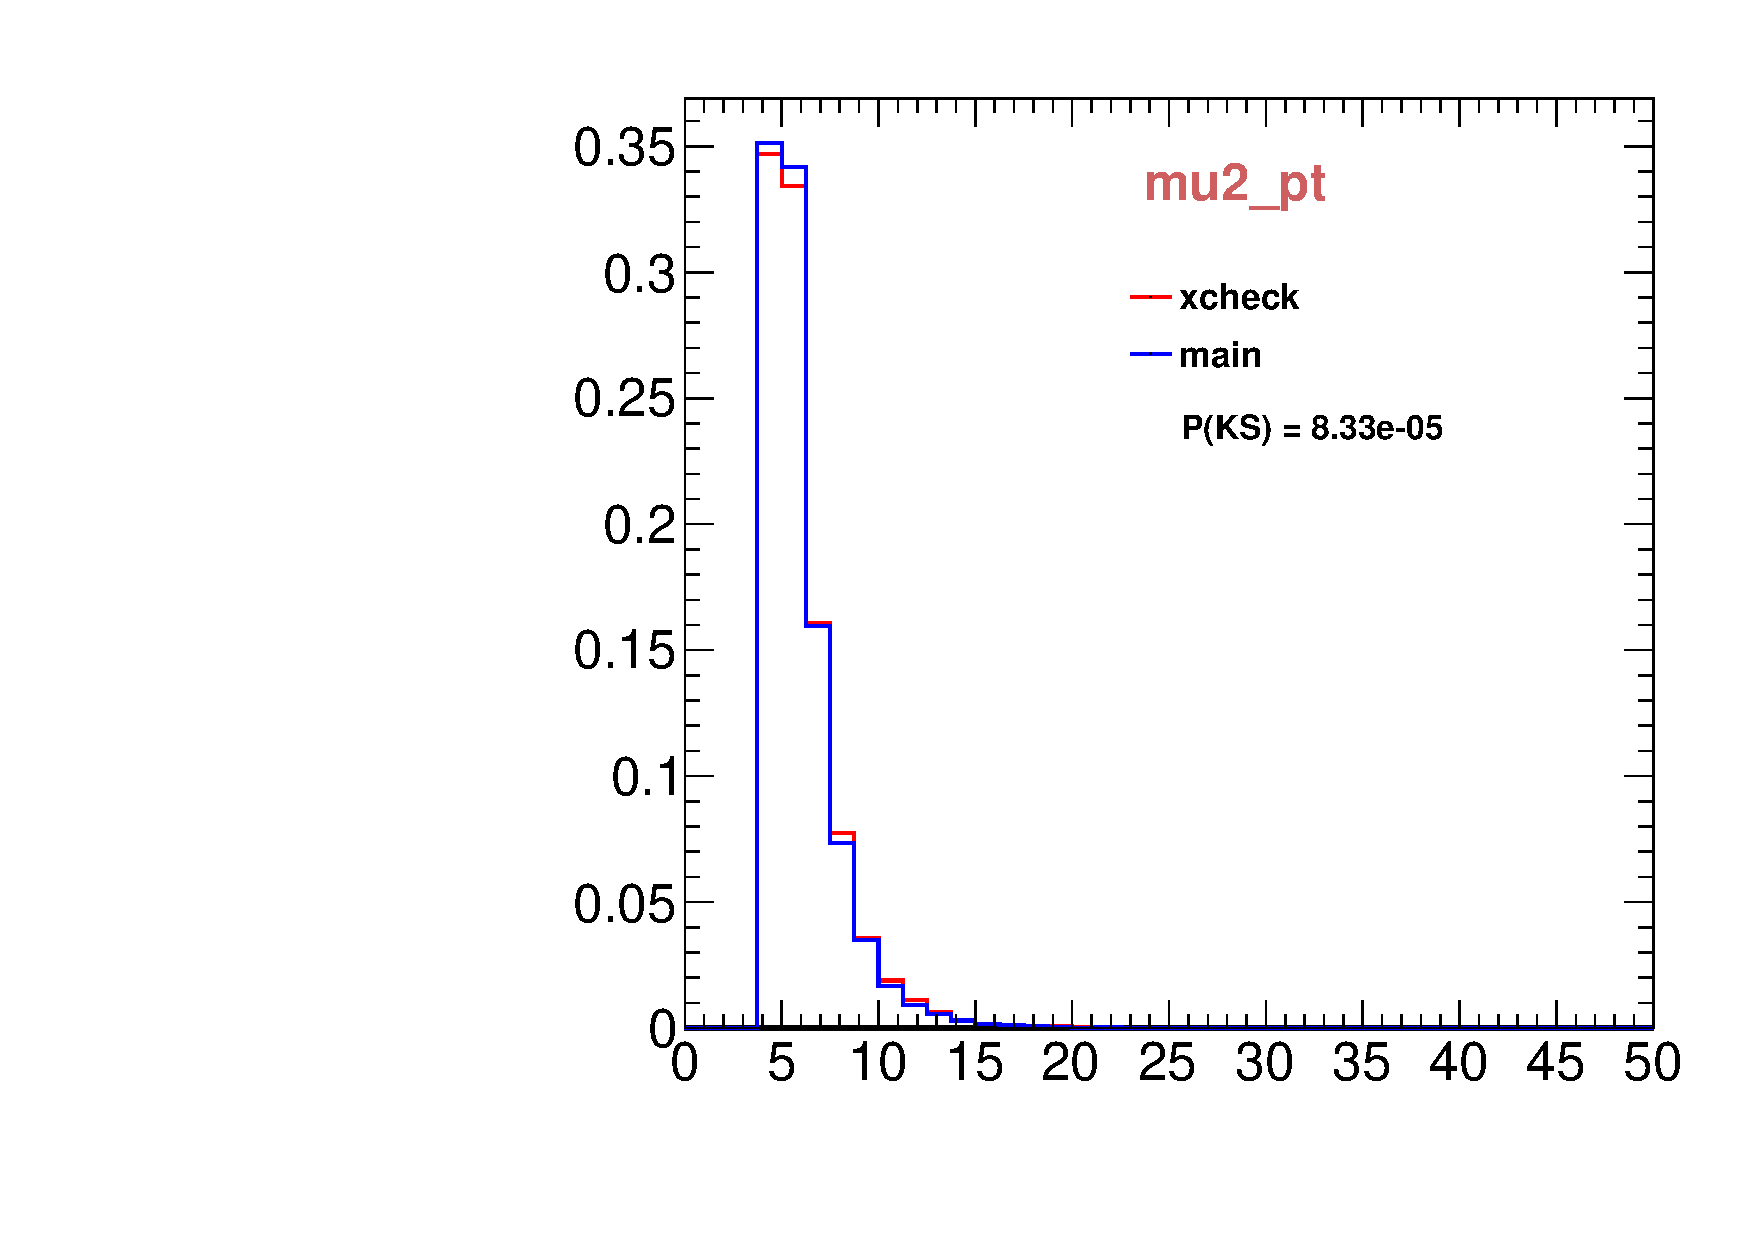
\includegraphics[width=\textwidth]{Figures/VariablesComparison/Data_barrel_figs/m2pt}
                \label{fig:Data_barrel_m2pt}
        \end{subfigure}
        \begin{subfigure}[b]{0.2\textwidth}
                \centering
                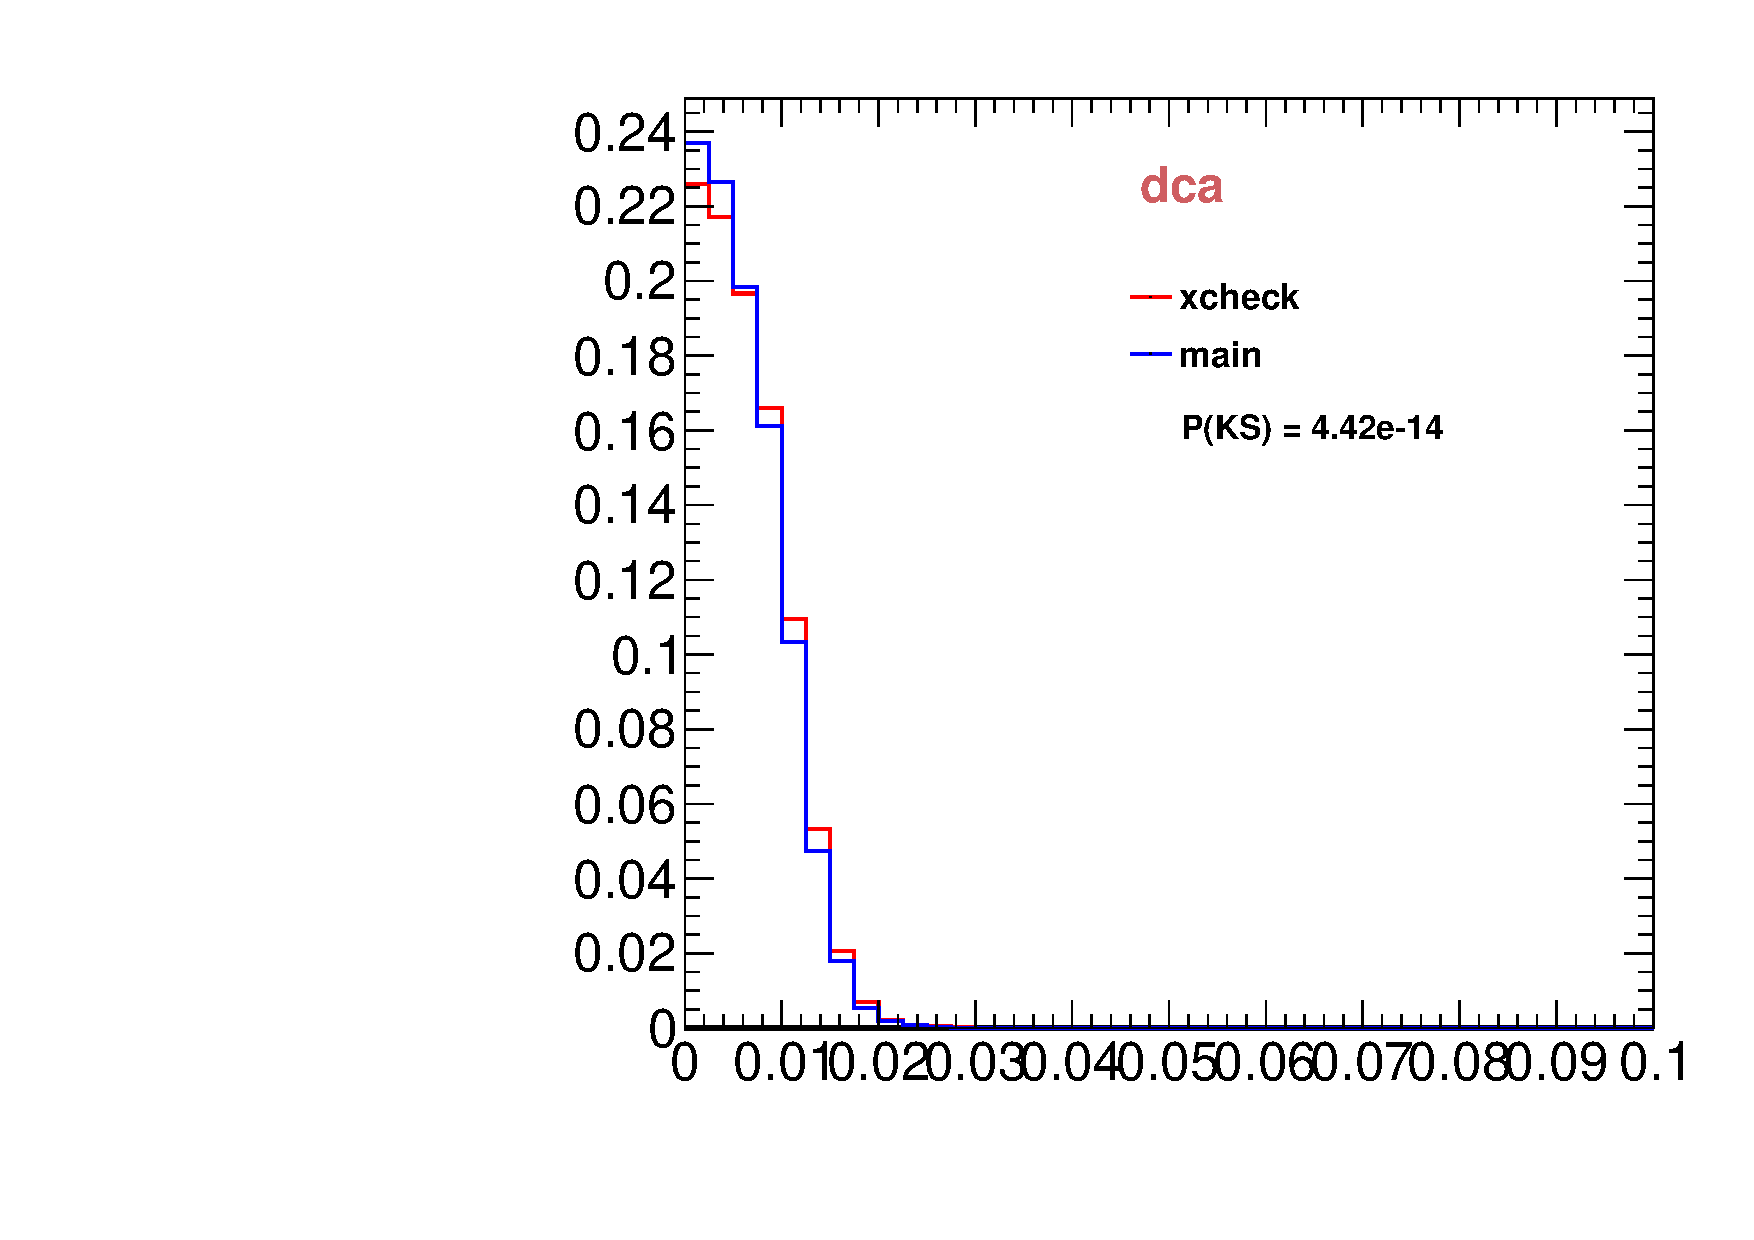
\includegraphics[width=\textwidth]{Figures/VariablesComparison/Data_barrel_figs/maxdoca}
                \label{fig:Data_barrel_maxdoca}
        \end{subfigure}
        \begin{subfigure}[b]{0.2\textwidth}
                \centering
                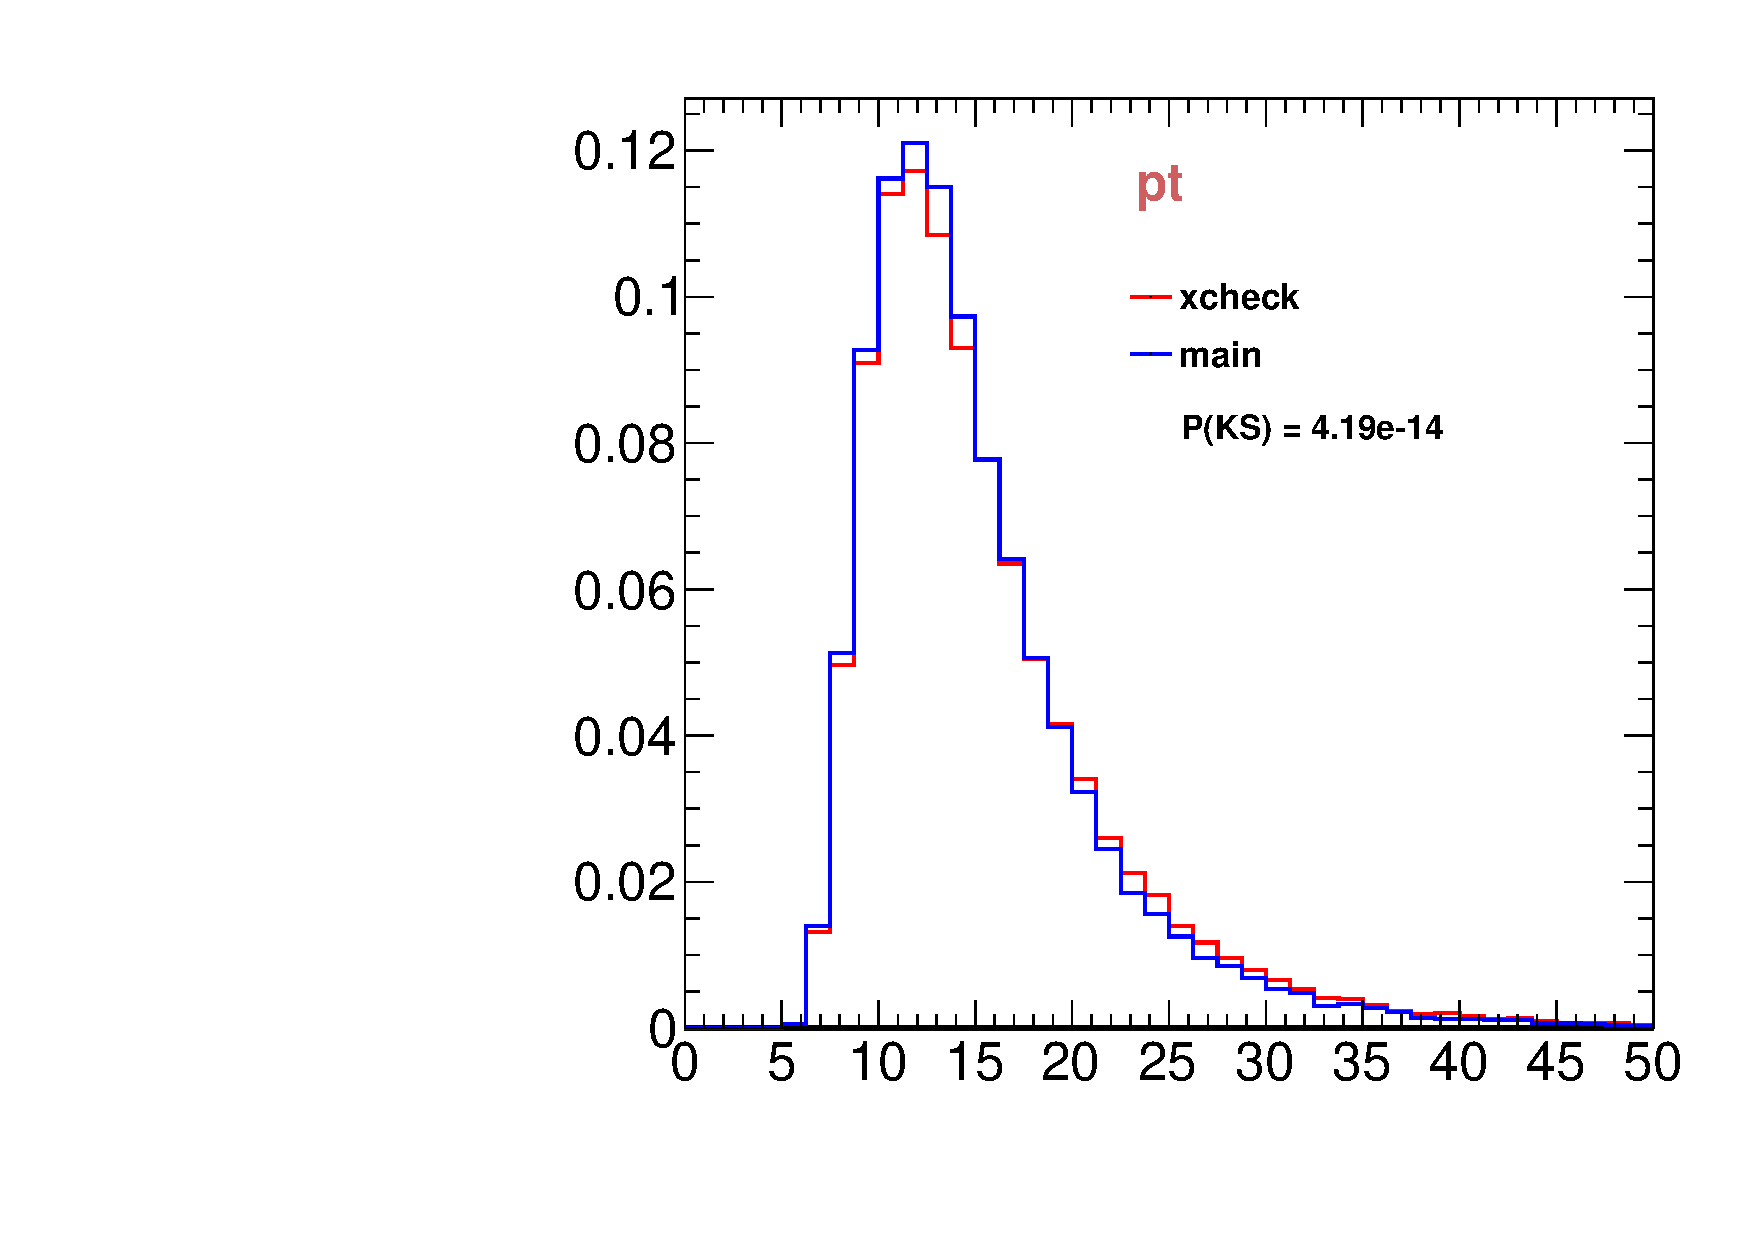
\includegraphics[width=\textwidth]{Figures/VariablesComparison/Data_barrel_figs/pt}
                \label{fig:Data_barrel_pt}
        \end{subfigure}
        \begin{subfigure}[b]{0.2\textwidth}
                \centering
                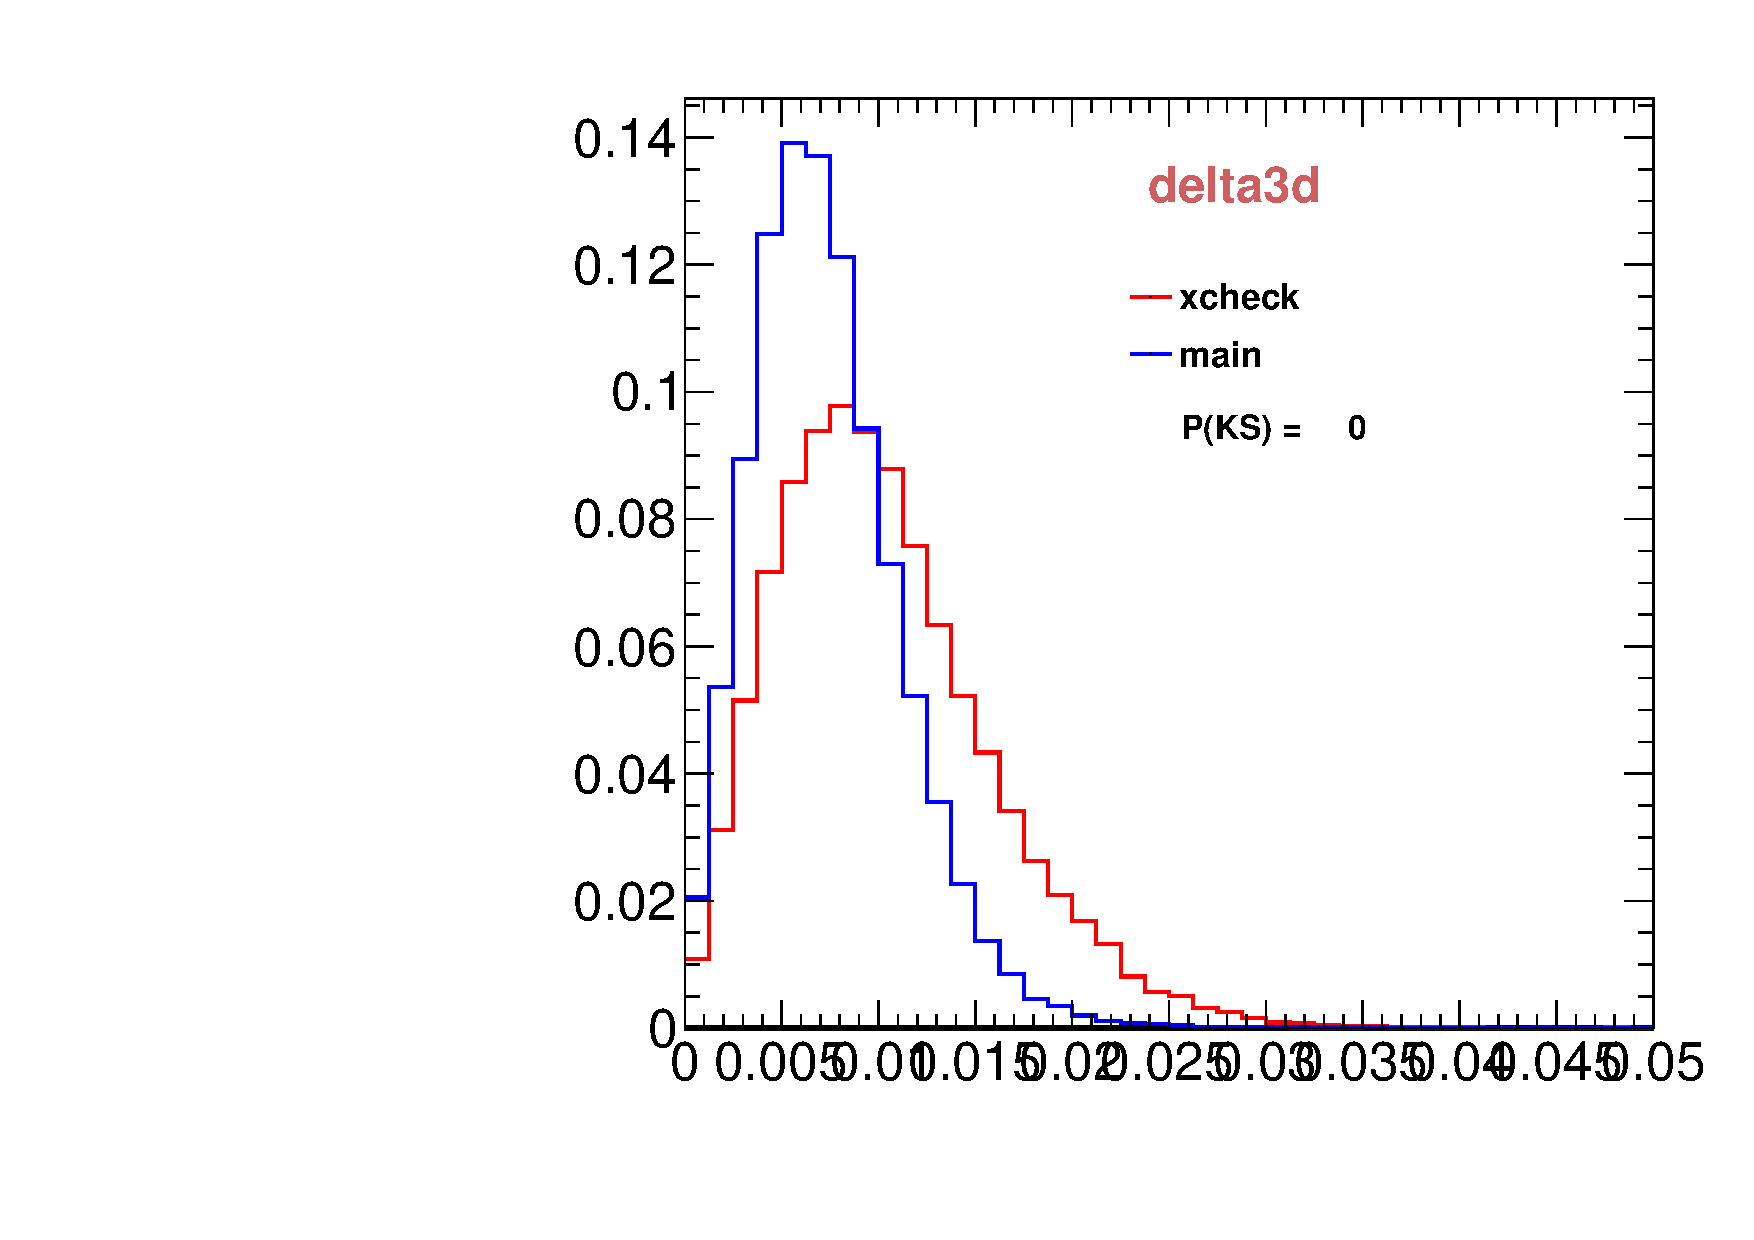
\includegraphics[width=\textwidth]{Figures/VariablesComparison/Data_barrel_figs/pvip}
                \label{fig:Data_barrel_pvip}
        \end{subfigure}
        \begin{subfigure}[b]{0.2\textwidth}
                \centering
                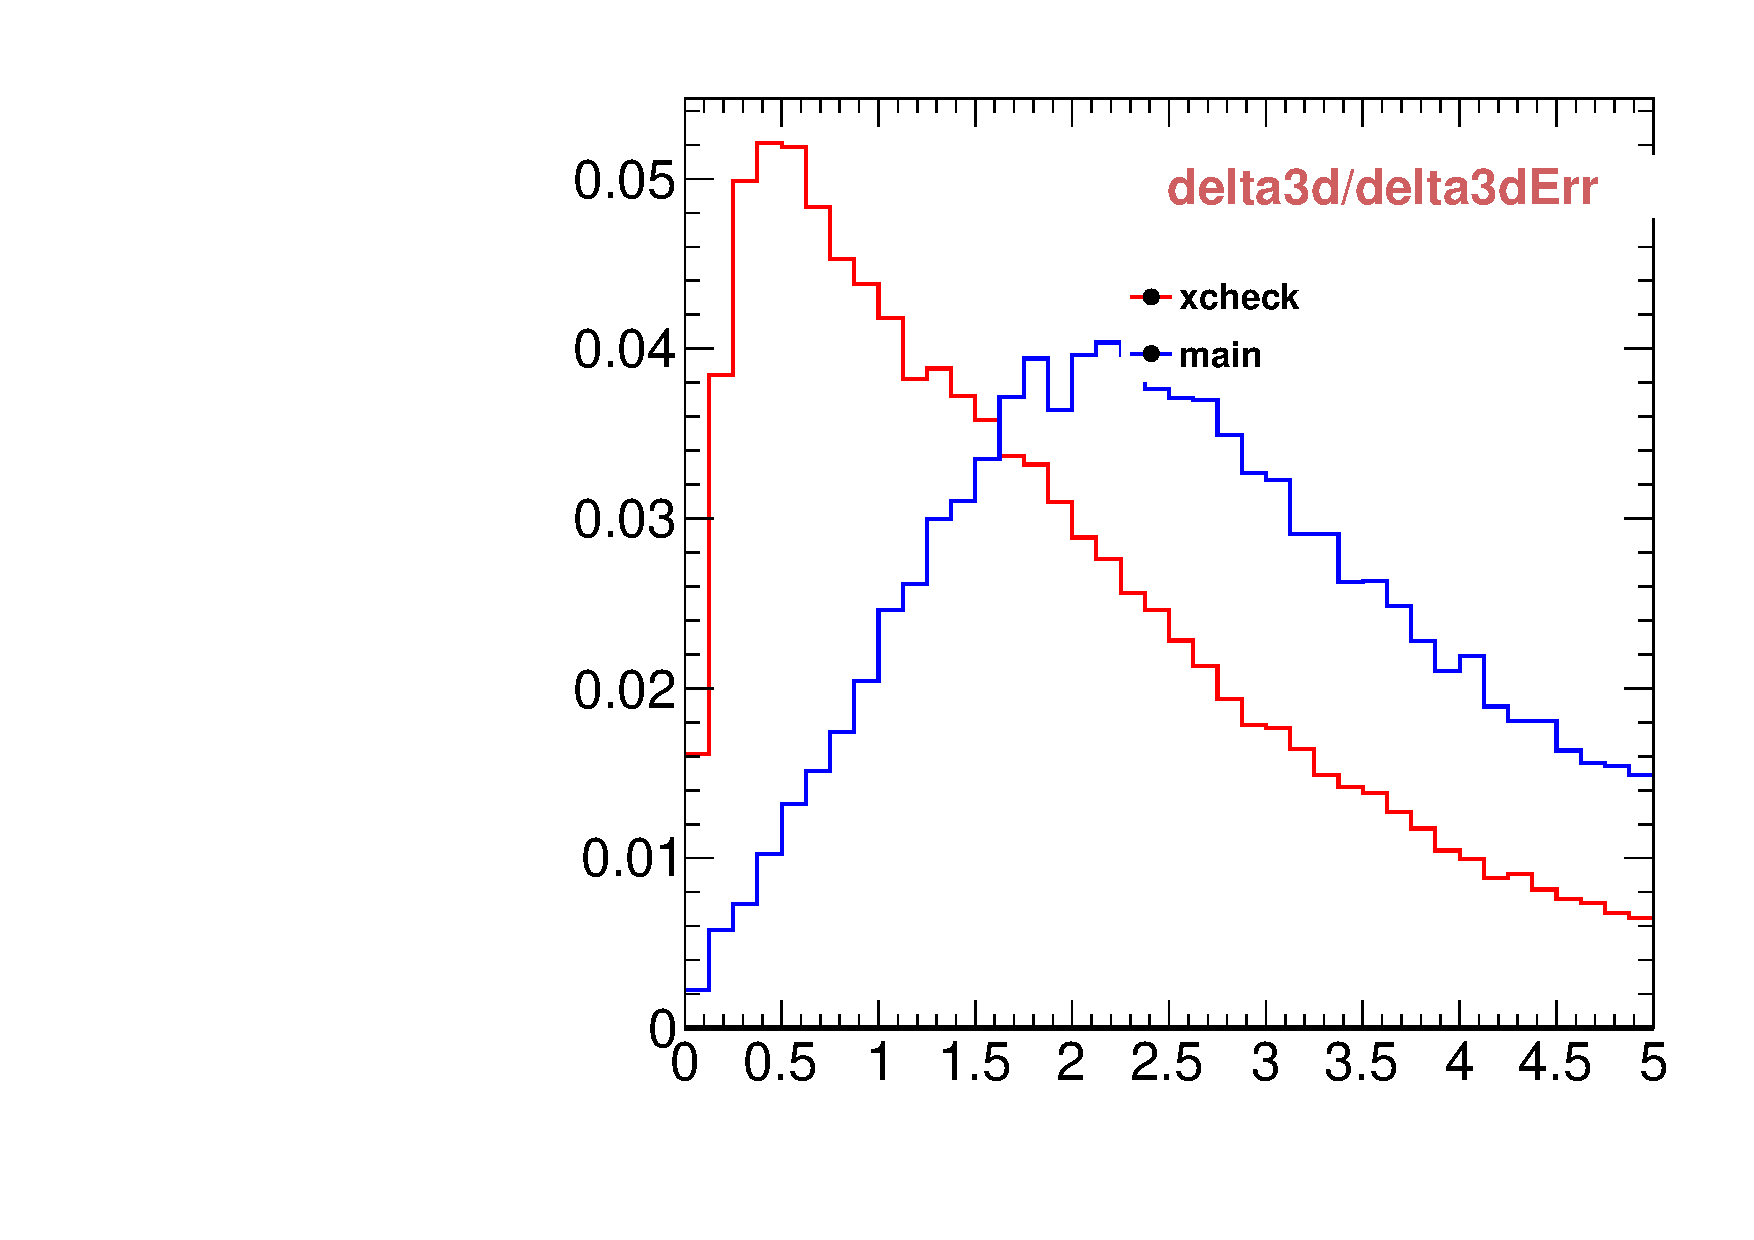
\includegraphics[width=\textwidth]{Figures/VariablesComparison/Data_barrel_figs/pvips}
                \label{fig:Data_barrel_pvips}
        \end{subfigure}
        \begin{subfigure}[b]{0.2\textwidth}
                \centering
                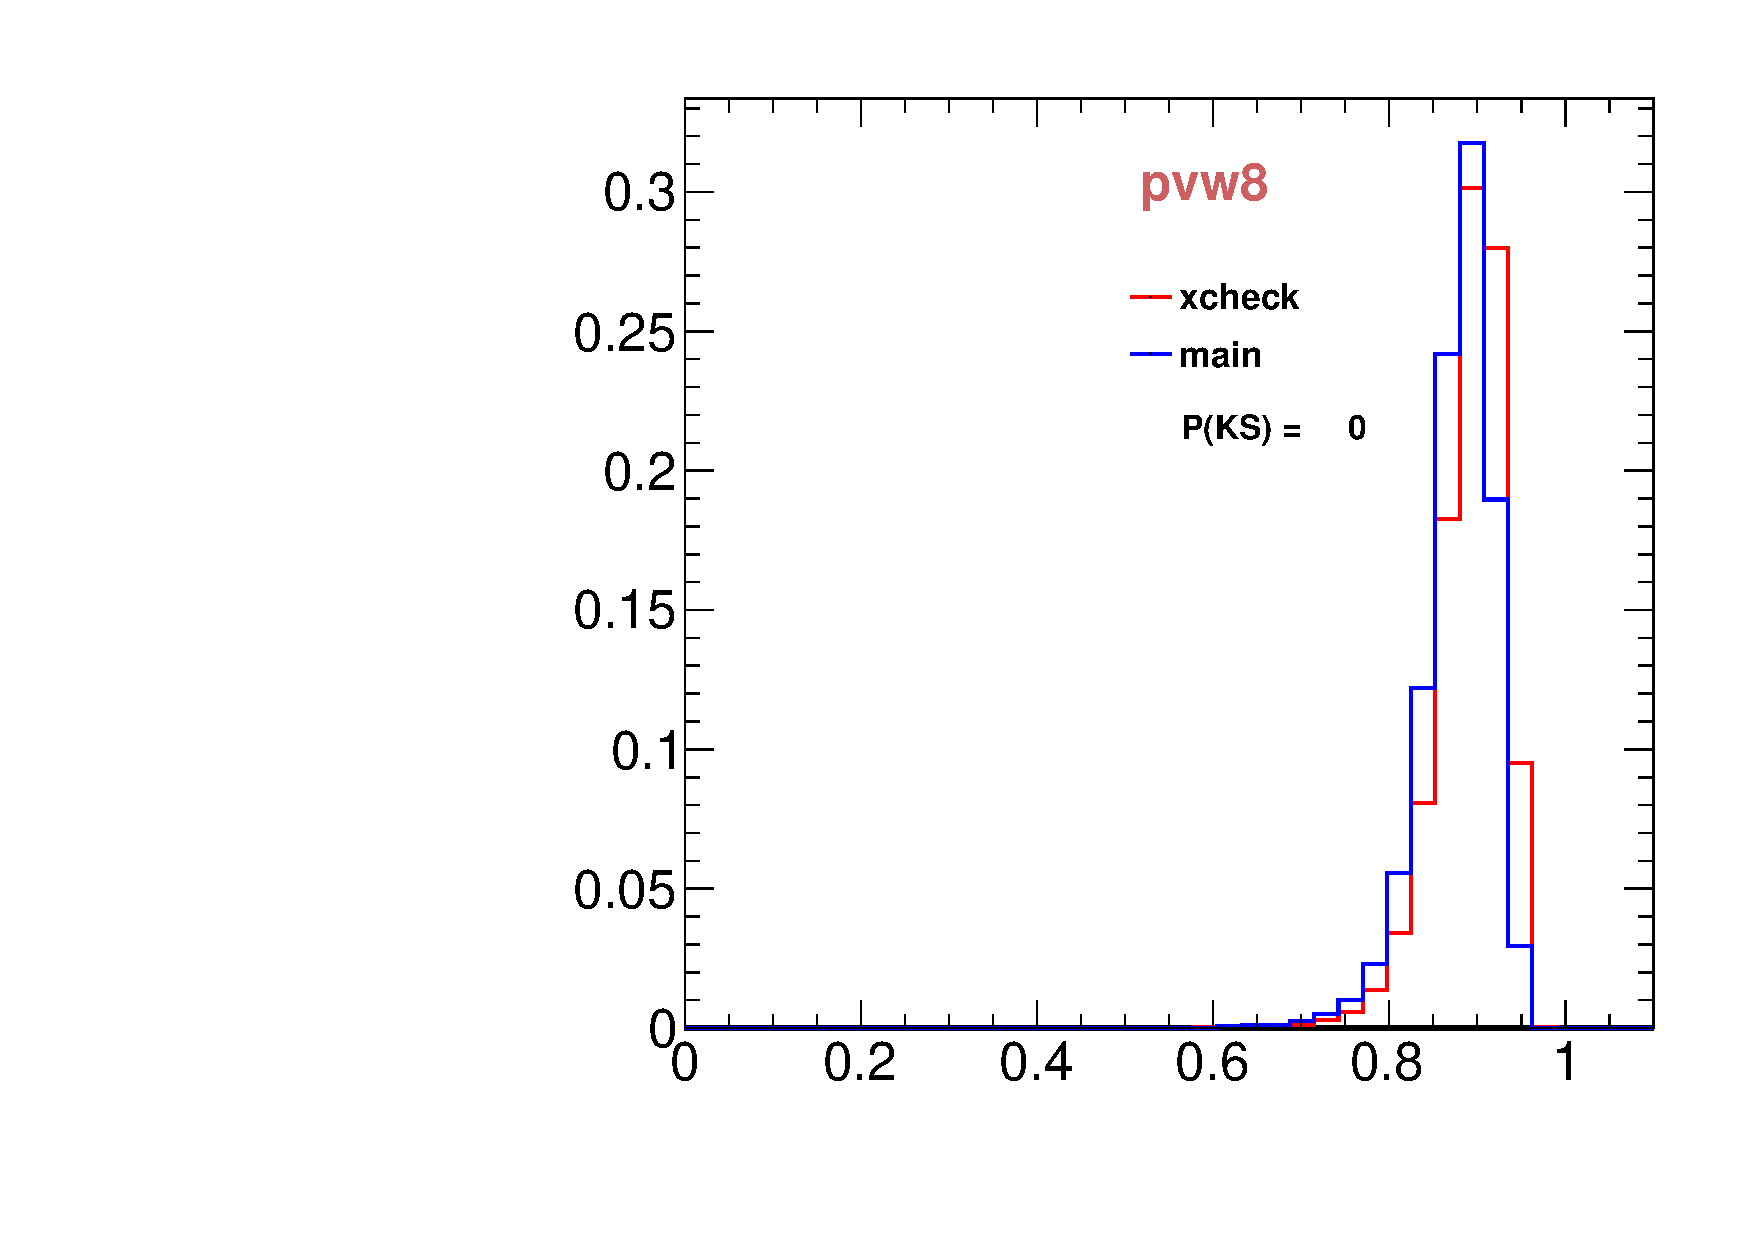
\includegraphics[width=\textwidth]{Figures/VariablesComparison/Data_barrel_figs/pvw8}
                \label{fig:Data_barrel_pvw8}
        \end{subfigure}
        \caption{Variable comparisons between the main analysis and the cross-check analysis. Part I: Data barrel.}
        \label{fig:Data_barrel_figs}
\end{sidewaysfigure}


\begin{sidewaysfigure}
        \centering
        \begin{subfigure}[b]{0.2\textwidth}
                \centering
                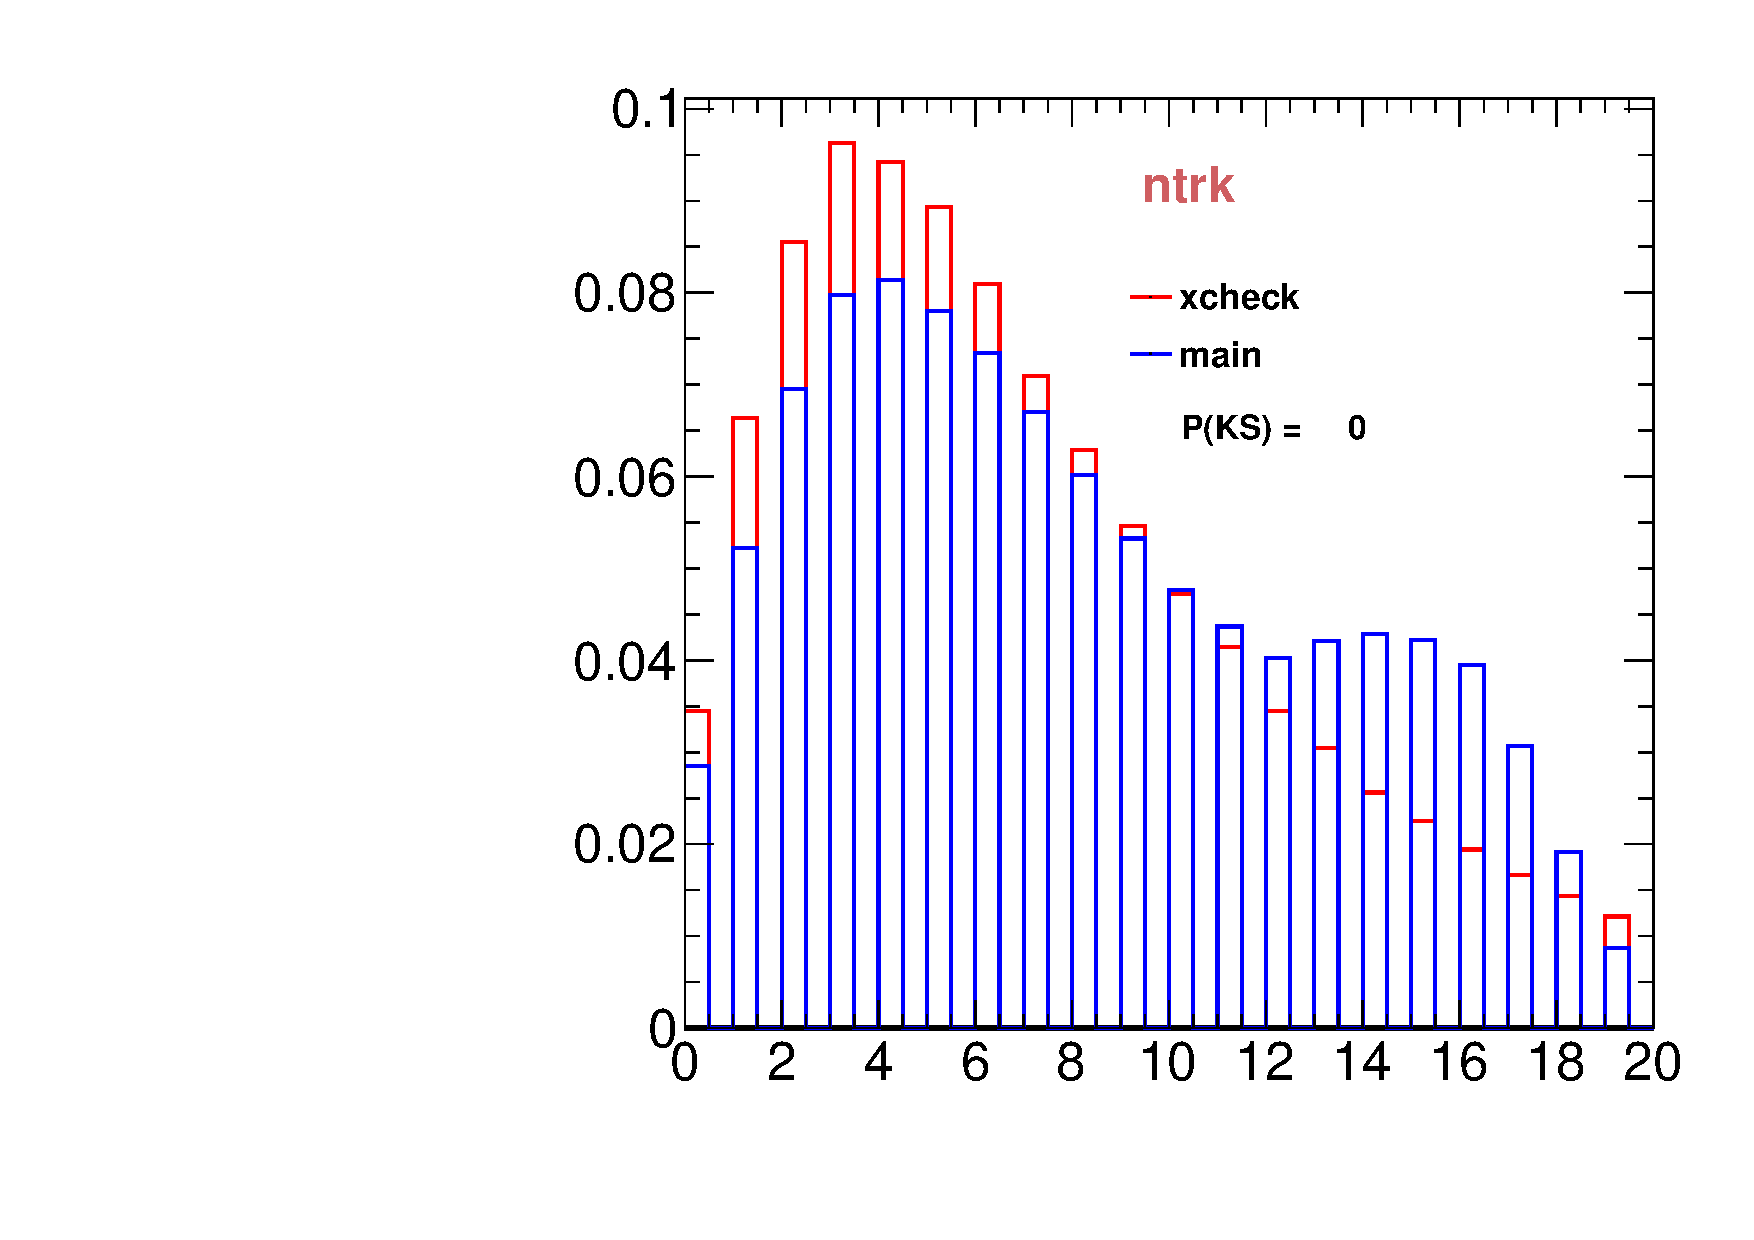
\includegraphics[width=\textwidth]{Figures/VariablesComparison/Data_endcaps_figs/closetrk}
                \label{fig:Data_endcaps_closetrk}
        \end{subfigure}
        \begin{subfigure}[b]{0.2\textwidth}
                \centering
                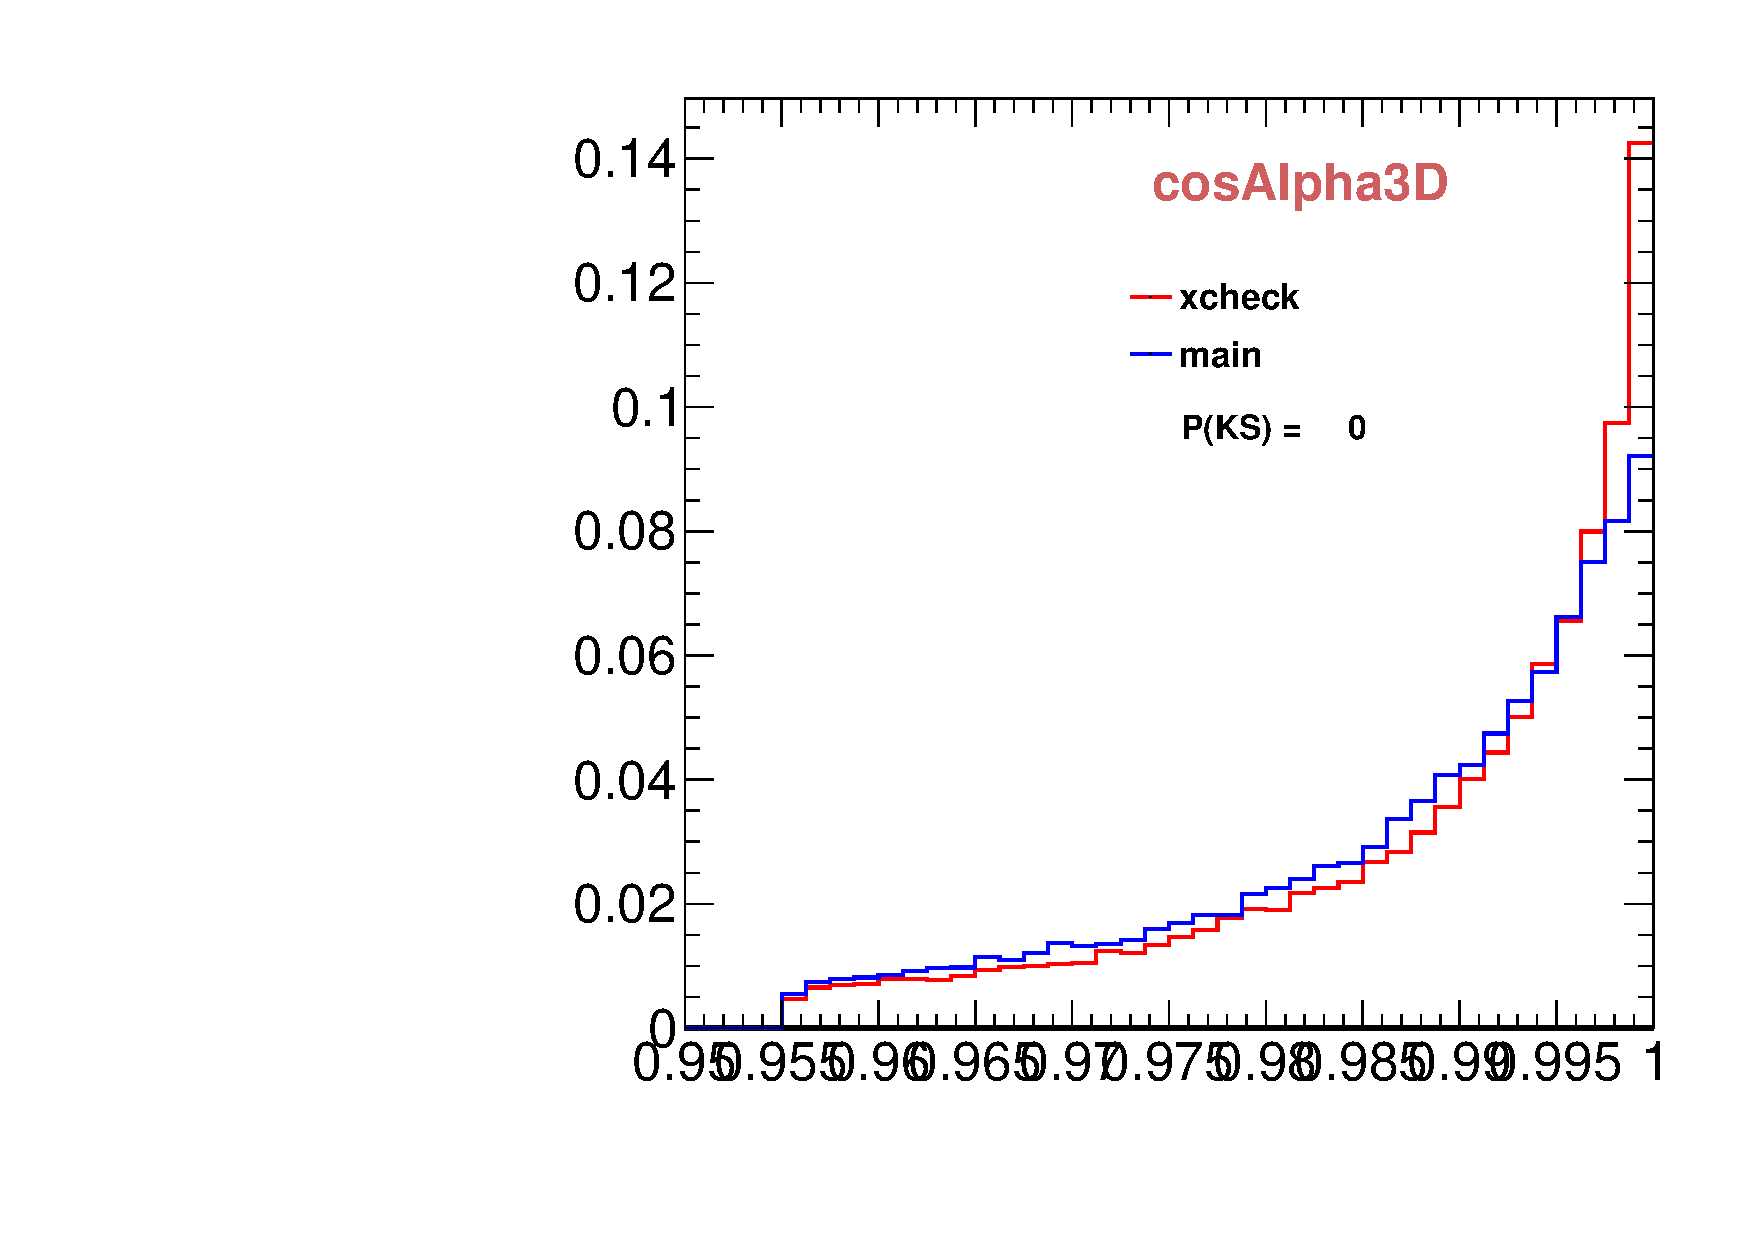
\includegraphics[width=\textwidth]{Figures/VariablesComparison/Data_endcaps_figs/cosa}
                \label{fig:Data_endcaps_cosa}
        \end{subfigure}
        \begin{subfigure}[b]{0.2\textwidth}
                \centering
                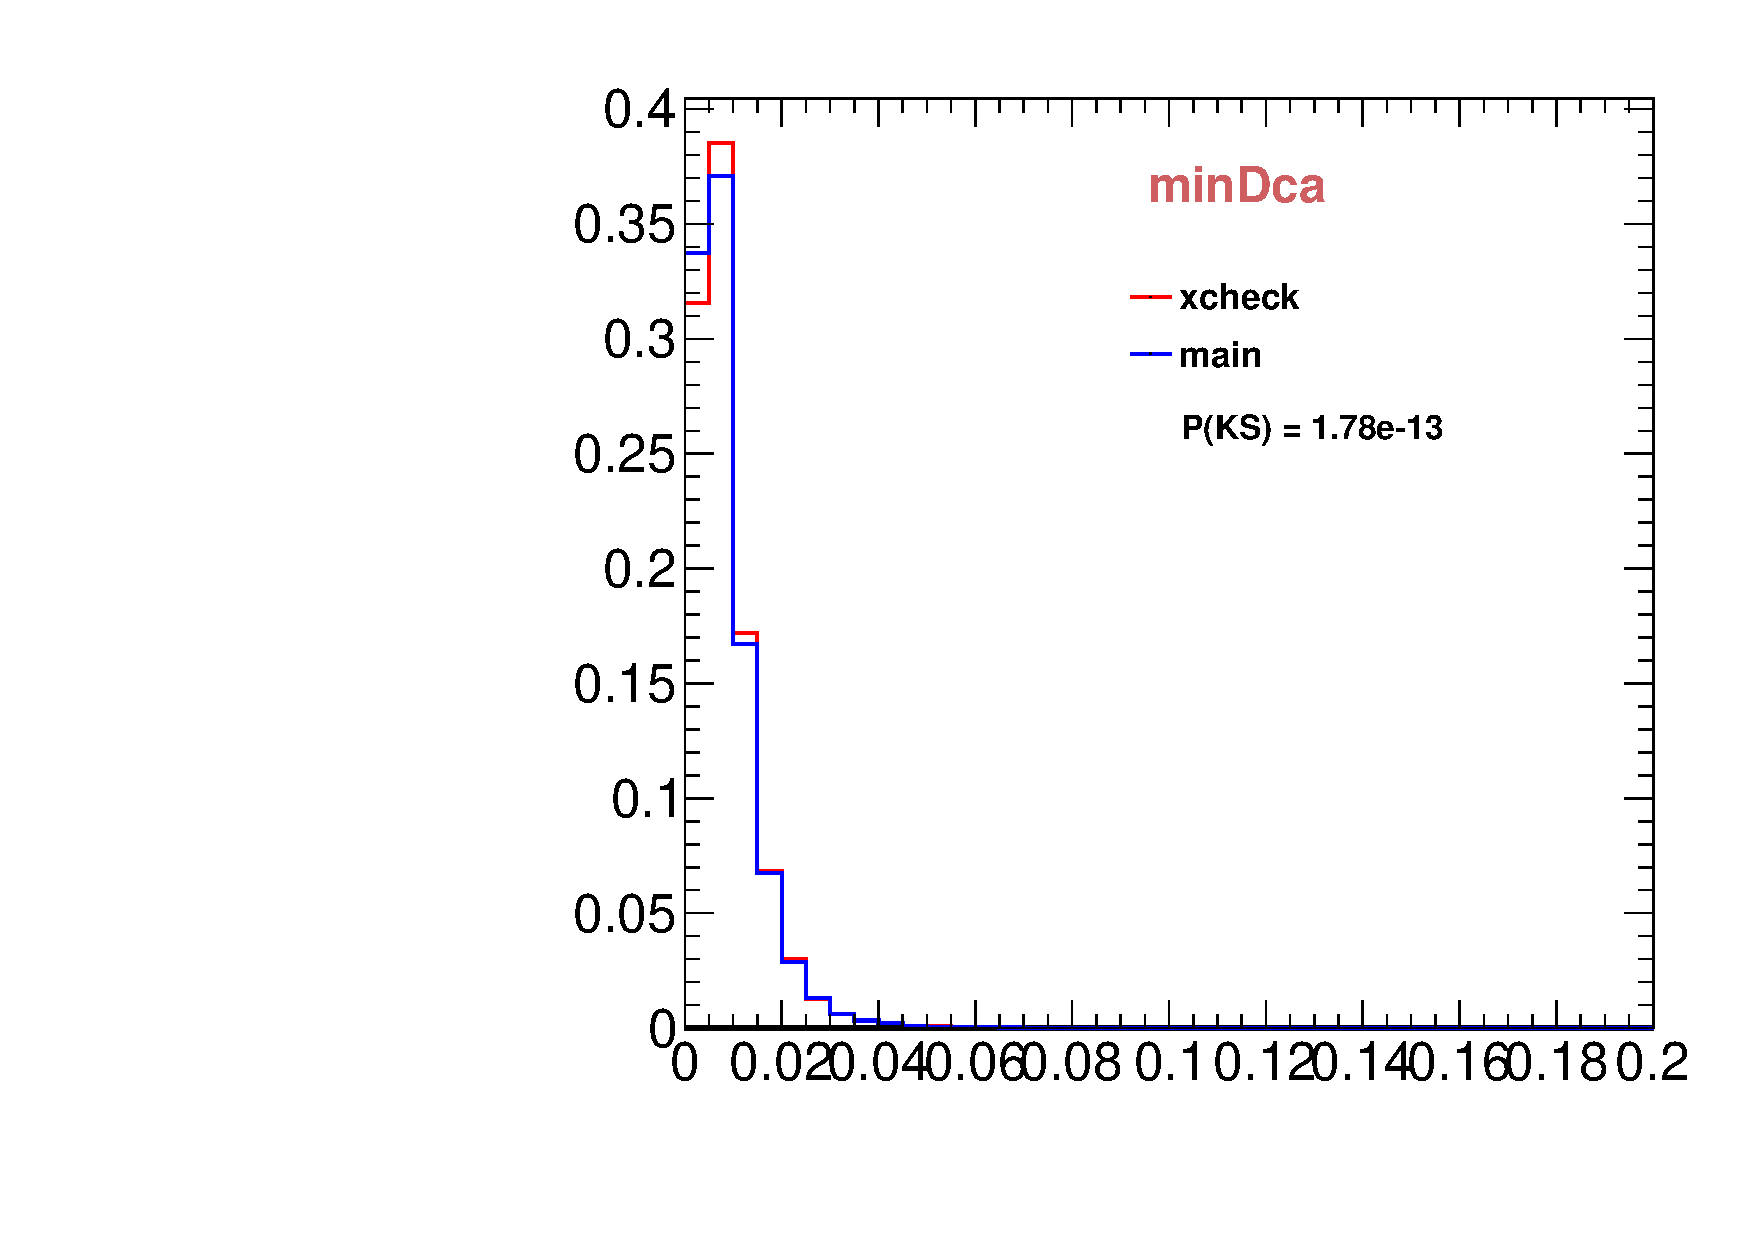
\includegraphics[width=\textwidth]{Figures/VariablesComparison/Data_endcaps_figs/docatrk}
                \label{fig:Data_endcaps_docatrk}
        \end{subfigure}
        \begin{subfigure}[b]{0.2\textwidth}
                \centering
                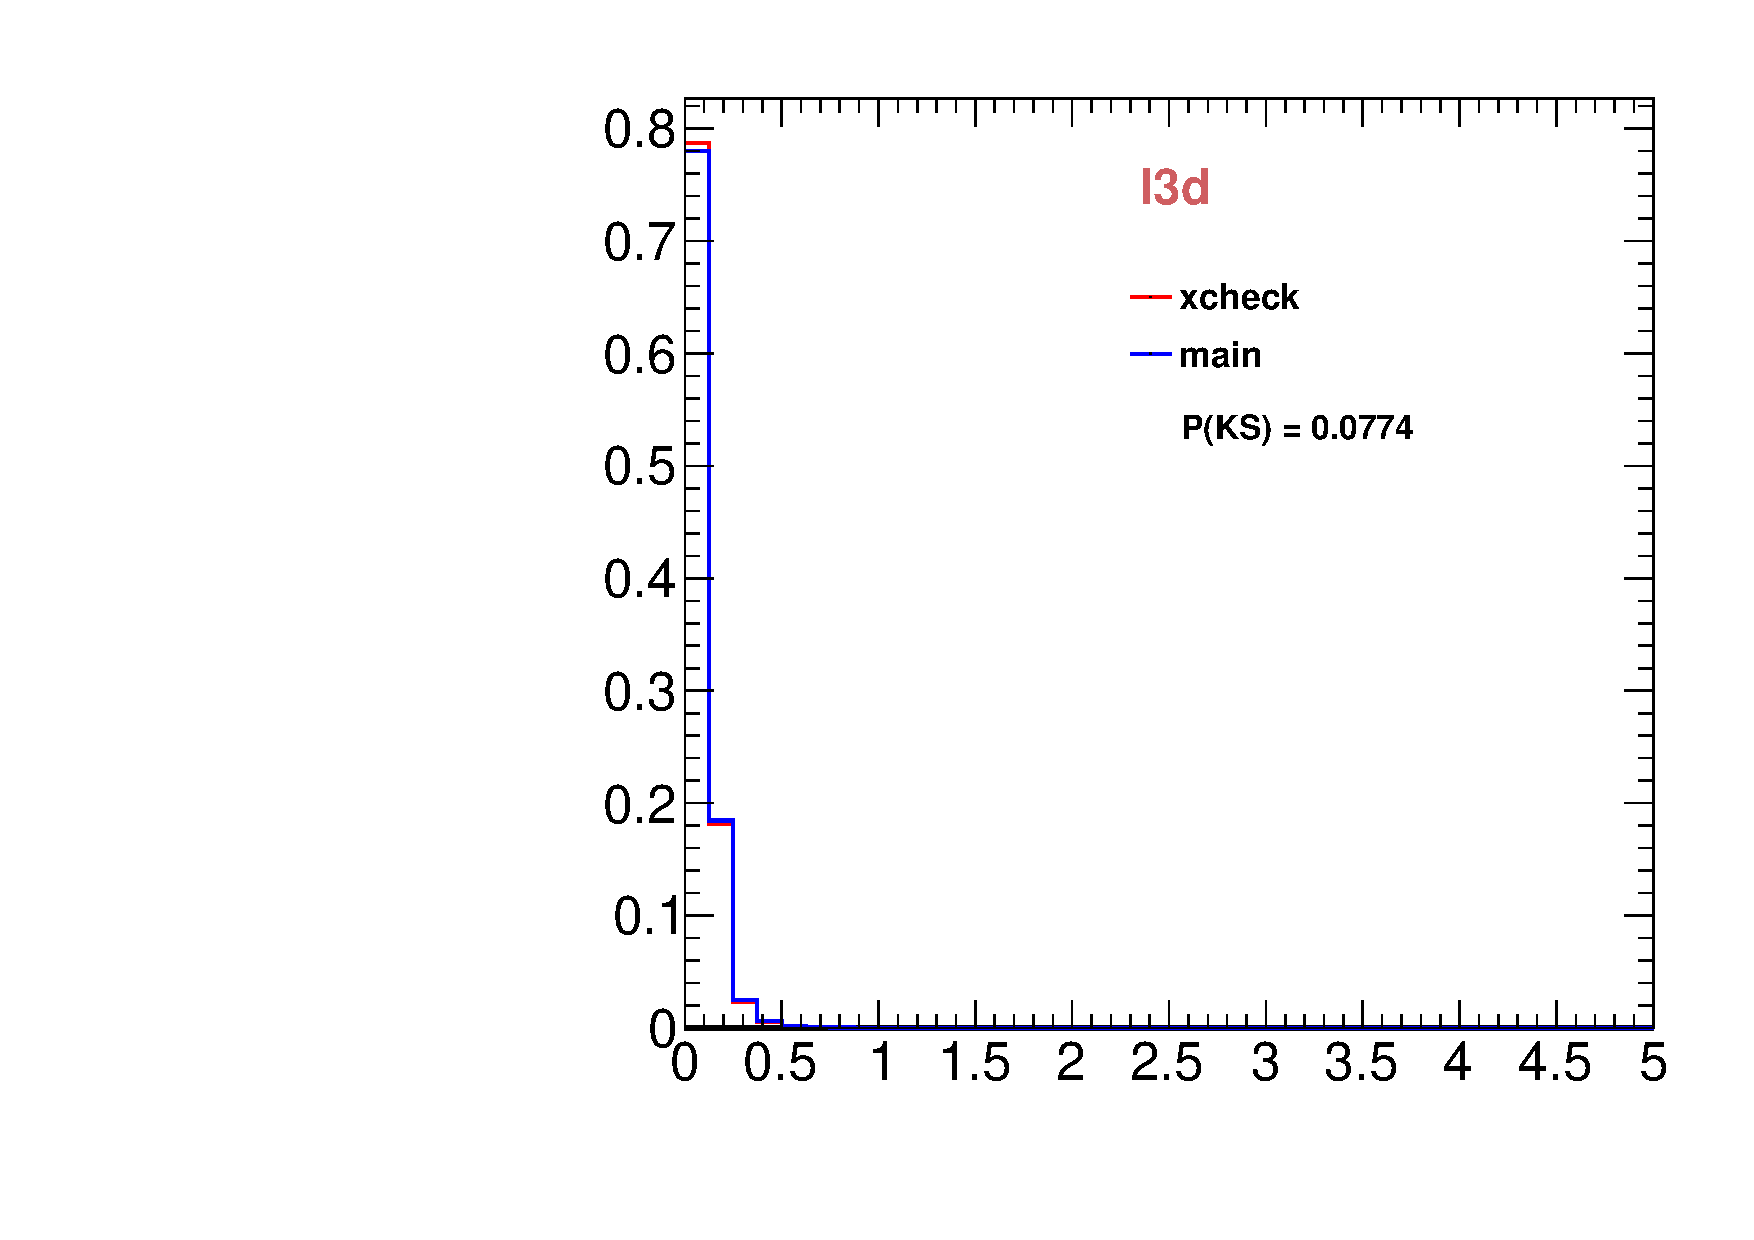
\includegraphics[width=\textwidth]{Figures/VariablesComparison/Data_endcaps_figs/fl3d}
                \label{fig:Data_endcaps_fl3d}
        \end{subfigure}
        \begin{subfigure}[b]{0.2\textwidth}
                \centering
                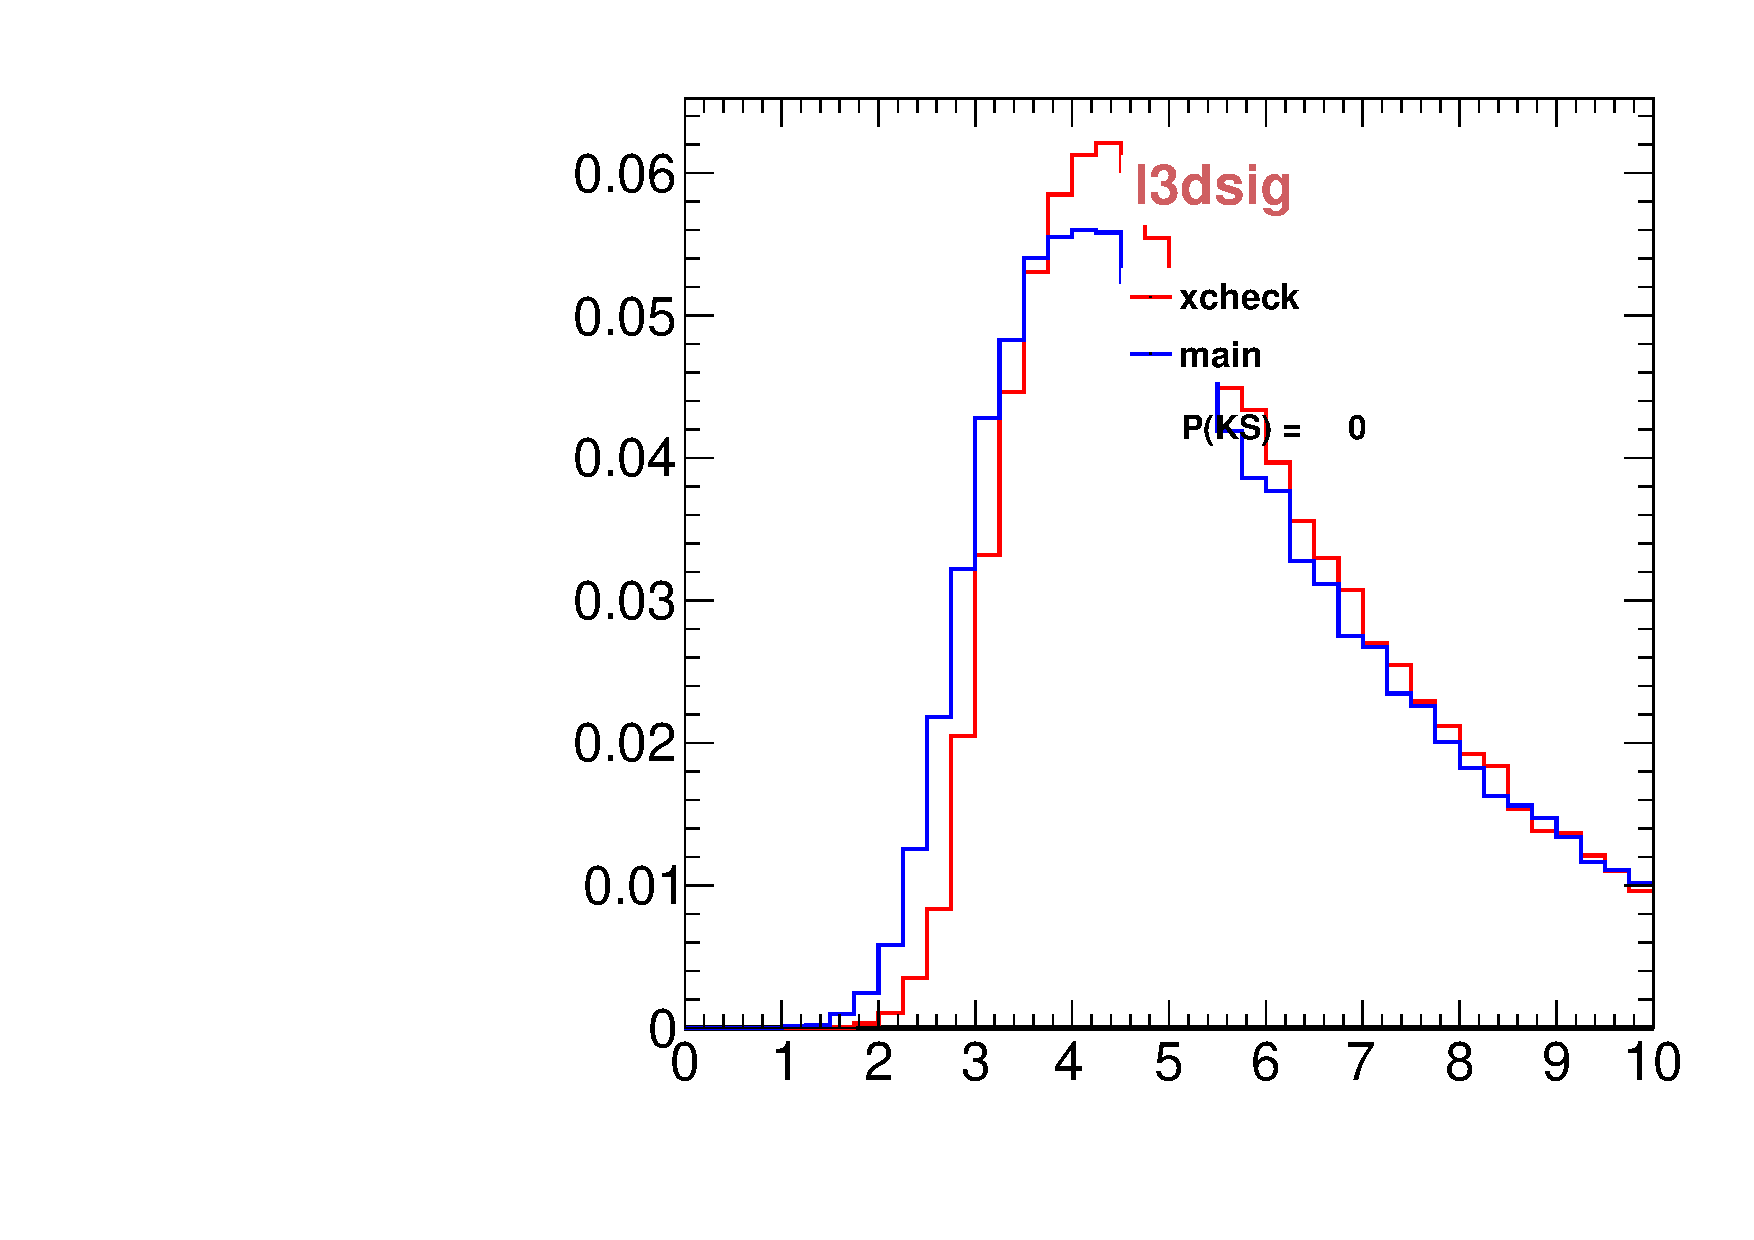
\includegraphics[width=\textwidth]{Figures/VariablesComparison/Data_endcaps_figs/fls3d}
                \label{fig:Data_endcaps_fls3d}
        \end{subfigure}
        \begin{subfigure}[b]{0.2\textwidth}
                \centering
                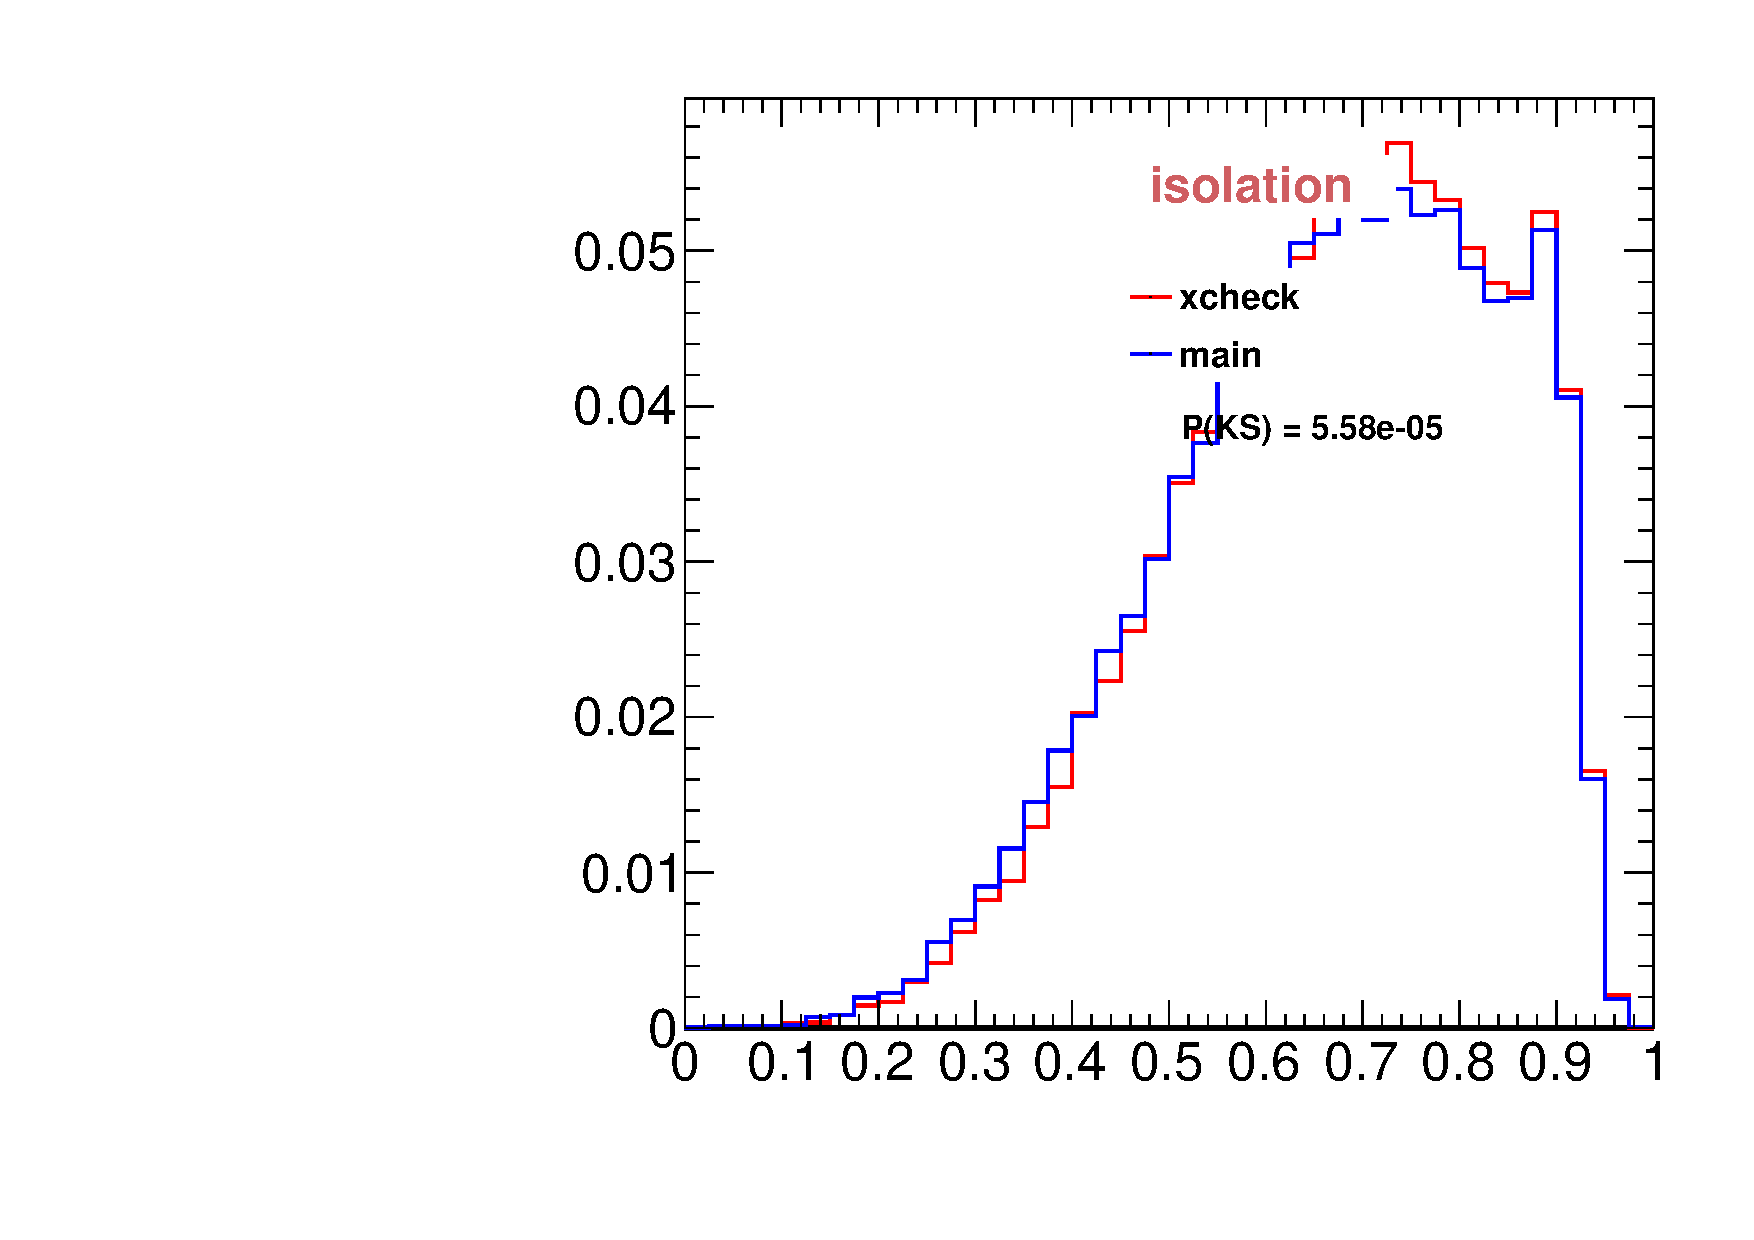
\includegraphics[width=\textwidth]{Figures/VariablesComparison/Data_endcaps_figs/iso}
                \label{fig:Data_endcaps_iso}
        \end{subfigure}
        \begin{subfigure}[b]{0.2\textwidth}
                \centering
                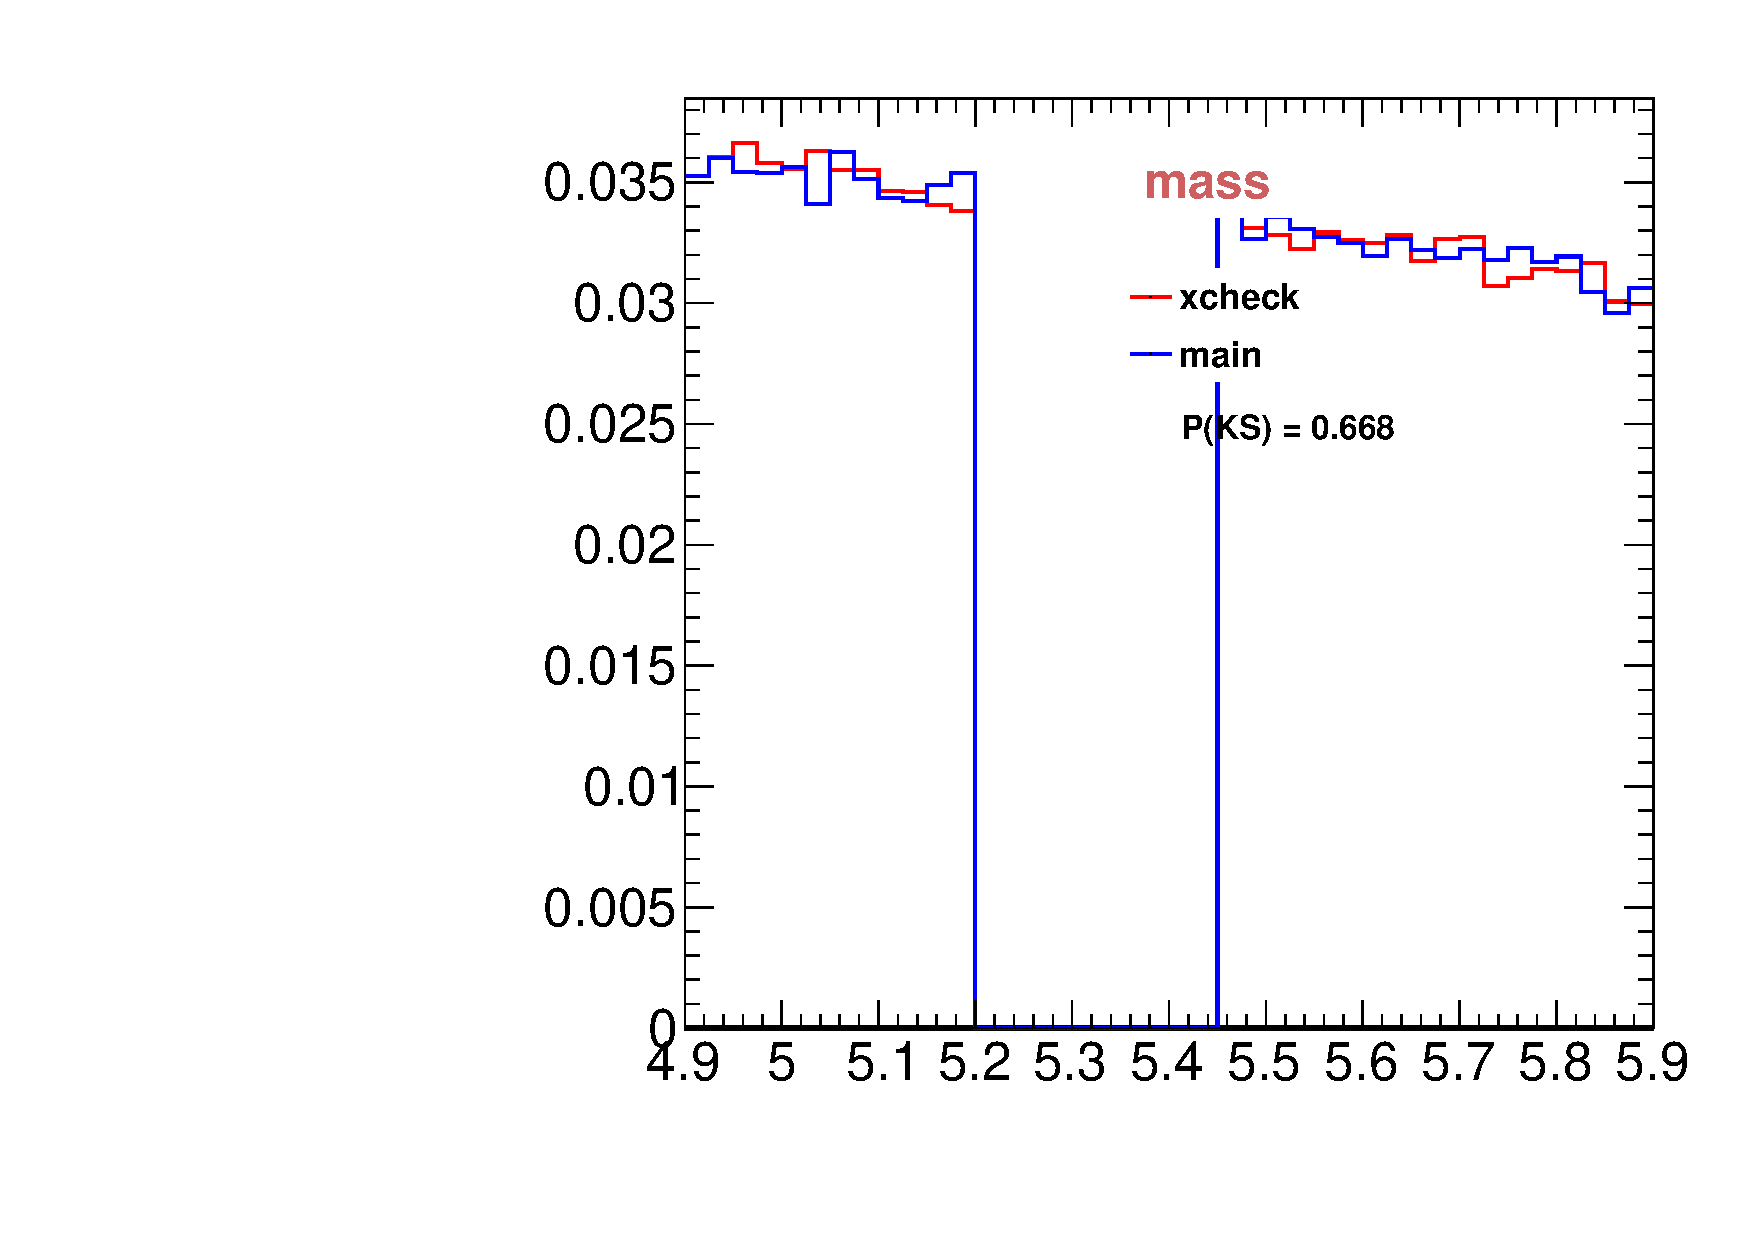
\includegraphics[width=\textwidth]{Figures/VariablesComparison/Data_endcaps_figs/m}
                \label{fig:Data_endcaps_m}
        \end{subfigure}
        \begin{subfigure}[b]{0.2\textwidth}
                \centering
                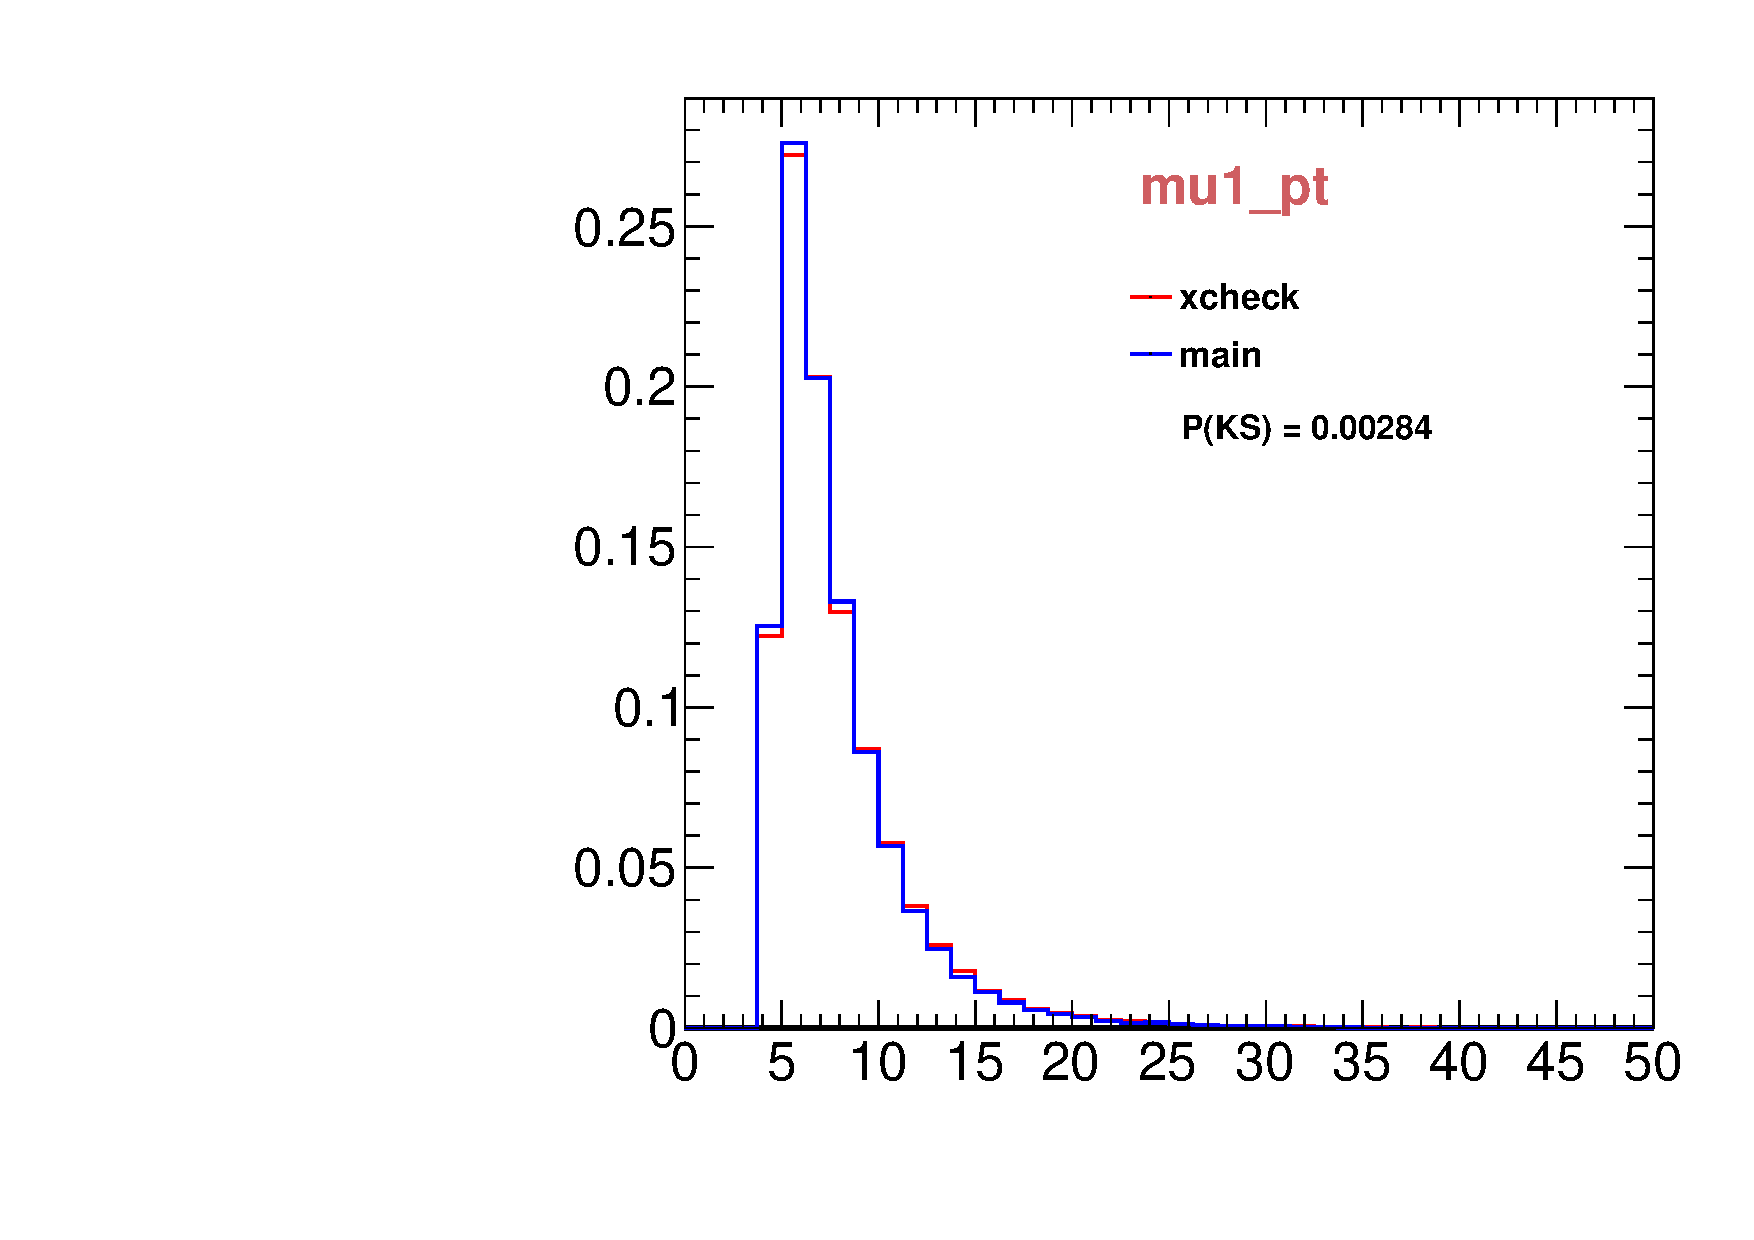
\includegraphics[width=\textwidth]{Figures/VariablesComparison/Data_endcaps_figs/m1pt}
                \label{fig:Data_endcaps_m1pt}
        \end{subfigure}
        \begin{subfigure}[b]{0.2\textwidth}
                \centering
                \includegraphics[width=\textwidth]{Figures/VariablesComparison/Data_endcaps_figs/m2pt}
                \label{fig:Data_endcaps_m2pt}
        \end{subfigure}
        \begin{subfigure}[b]{0.2\textwidth}
                \centering
                \includegraphics[width=\textwidth]{Figures/VariablesComparison/Data_endcaps_figs/maxdoca}
                \label{fig:Data_endcaps_maxdoca}
        \end{subfigure}
        \begin{subfigure}[b]{0.2\textwidth}
                \centering
                \includegraphics[width=\textwidth]{Figures/VariablesComparison/Data_endcaps_figs/pt}
                \label{fig:Data_endcaps_pt}
        \end{subfigure}
        \begin{subfigure}[b]{0.2\textwidth}
                \centering
                \includegraphics[width=\textwidth]{Figures/VariablesComparison/Data_endcaps_figs/pvip}
                \label{fig:Data_endcaps_pvip}
        \end{subfigure}
        \begin{subfigure}[b]{0.2\textwidth}
                \centering
                \includegraphics[width=\textwidth]{Figures/VariablesComparison/Data_endcaps_figs/pvips}
                \label{fig:Data_endcaps_pvips}
        \end{subfigure}
        \begin{subfigure}[b]{0.2\textwidth}
                \centering
                \includegraphics[width=\textwidth]{Figures/VariablesComparison/Data_endcaps_figs/pvw8}
                \label{fig:Data_endcaps_pvw8}
        \end{subfigure}
        \caption{Variable comparisons between the main analysis and the cross-check analysis. Part I: Data endcaps.}
        \label{fig:Data_endcaps_figs}
\end{sidewaysfigure}


